\documentclass[11pt,a4paper]{article}

% =============================================================================
% Packages
% =============================================================================
\usepackage[utf8]{inputenc}
\usepackage[spanish,es-tabla,es-nodecimaldot]{babel}
\usepackage[margin=2.5cm]{geometry}
\usepackage{xcolor}
\usepackage{hyperref}
\usepackage{fancyhdr}
\usepackage{titlesec}
\usepackage{enumitem}
\usepackage{listings}
\usepackage{tabularx}
\usepackage{longtable}
\usepackage{booktabs}
\usepackage{array}
\usepackage{parskip}
\usepackage{graphicx}
\usepackage{float}
\graphicspath{{manual_assets/}}

% =============================================================================
% Colors
% =============================================================================
\definecolor{valuedataverde}{RGB}{21,147,73}
\definecolor{falabellaamarillo}{RGB}{255,203,5}
\definecolor{grisclaro}{RGB}{240,240,240}
\definecolor{grismedio}{RGB}{200,200,200}
\definecolor{rojoaviso}{RGB}{200,40,40}
\definecolor{azulinfo}{RGB}{30,90,170}

% =============================================================================
% Hyperref
% =============================================================================
\hypersetup{
  colorlinks=true,
  linkcolor=valuedataverde,
  urlcolor=azulinfo,
  citecolor=valuedataverde,
  pdftitle={Manual de Usuario - ValueData x Falabella},
  pdfauthor={ValueData},
  pdfsubject={Manual de Usuario POC Falabella},
}

% =============================================================================
% Section colors
% =============================================================================
\titleformat{\section}
  {\color{valuedataverde}\Large\bfseries}{\thesection}{0.6em}{}
\titleformat{\subsection}
  {\color{valuedataverde!85!black}\large\bfseries}{\thesubsection}{0.5em}{}
\titleformat{\subsubsection}
  {\bfseries}{\thesubsubsection}{0.4em}{}

% =============================================================================
% Header / footer
% =============================================================================
\pagestyle{fancy}
\fancyhf{}
\fancyhead[L]{\small\color{valuedataverde}\textbf{Manual de Usuario}}
\fancyhead[R]{\small ValueData $\times$ Falabella}
\fancyfoot[C]{\thepage}
\renewcommand{\headrulewidth}{0.4pt}
\renewcommand{\footrulewidth}{0pt}

% =============================================================================
% Listings (CSV / curl / JSON)
% =============================================================================
\lstset{
  basicstyle=\ttfamily\small,
  backgroundcolor=\color{grisclaro},
  frame=single,
  rulecolor=\color{grismedio},
  breaklines=true,
  breakatwhitespace=true,
  columns=fullflexible,
  showstringspaces=false,
  postbreak=\mbox{\textcolor{grismedio}{$\hookrightarrow$}\space},
  literate={á}{{\'a}}1 {é}{{\'e}}1 {í}{{\'i}}1 {ó}{{\'o}}1 {ú}{{\'u}}1
           {Á}{{\'A}}1 {É}{{\'E}}1 {Í}{{\'I}}1 {Ó}{{\'O}}1 {Ú}{{\'U}}1
           {ñ}{{\~n}}1 {Ñ}{{\~N}}1 {¿}{{?`}}1 {¡}{{!`}}1
           {°}{{$^{\circ}$}}1 {º}{{$^{\circ}$}}1
}

% =============================================================================
% Boxes destacados
% =============================================================================
\newcommand{\tipbox}[1]{%
  \par\medskip\noindent\fcolorbox{valuedataverde}{valuedataverde!8}{%
    \begin{minipage}{0.95\linewidth}\small
      \textbf{\color{valuedataverde}Tip.} #1
    \end{minipage}%
  }\par\medskip
}

\newcommand{\warnbox}[1]{%
  \par\medskip\noindent\fcolorbox{rojoaviso}{rojoaviso!8}{%
    \begin{minipage}{0.95\linewidth}\small
      \textbf{\color{rojoaviso}Atencion.} #1
    \end{minipage}%
  }\par\medskip
}

\newcommand{\importantbox}[1]{%
  \par\medskip\noindent\fcolorbox{falabellaamarillo!70!black}{falabellaamarillo!15}{%
    \begin{minipage}{0.95\linewidth}\small
      \textbf{Importante.} #1
    \end{minipage}%
  }\par\medskip
}

\newcommand{\wipbox}[1]{%
  \par\medskip\noindent\fcolorbox{azulinfo}{azulinfo!8}{%
    \begin{minipage}{0.95\linewidth}\small
      \textbf{\color{azulinfo}En desarrollo.} #1
    \end{minipage}%
  }\par\medskip
}

\setlist[enumerate,1]{leftmargin=*,itemsep=0.2em}
\setlist[itemize,1]{leftmargin=*,itemsep=0.2em}

% =============================================================================
% Title page
% =============================================================================
\title{%
  \vspace*{2cm}
  {\Huge\color{valuedataverde}\textbf{Manual de Usuario}}\\[0.6cm]
  {\LARGE ValueData $\times$ Falabella}\\[0.4cm]
  {\large Torre de control predictiva para entregas de ultima milla}
}
\author{ValueData --- Equipo Producto}
\date{Abril 2026}

\begin{document}

\begin{titlepage}
\centering
\vspace*{2.5cm}

{\color{valuedataverde}\rule{\linewidth}{1.2pt}}\\[0.4cm]
{\Huge\bfseries\color{valuedataverde} Manual de Usuario}\\[0.5cm]
{\LARGE ValueData $\times$ Falabella}\\[0.3cm]
{\color{valuedataverde}\rule{\linewidth}{0.6pt}}\\[0.6cm]

{\large Torre de control predictiva para entregas de ultima milla}\\[1.4cm]

{\large Version POC --- Abril 2026}\\[0.6cm]

\vspace{1cm}

\begin{minipage}{0.85\linewidth}\centering\itshape
Este manual describe paso a paso como operar la plataforma ValueData
configurada para Falabella. Esta dirigido al equipo de operaciones,
jefes de transporte, despachadores y choferes que usaran la herramienta
en el dia a dia. No requiere conocimientos tecnicos previos.
\end{minipage}

\vfill

\begin{tabular}{rl}
\textbf{Frontend:} & \url{https://flogging-purposely-antonym.ngrok-free.dev/} \\
\textbf{Backend:}  & \texttt{http://localhost:8090} \\
\textbf{Soporte:}  & equipo ValueData \\
\end{tabular}

\vspace{1cm}
\end{titlepage}

\tableofcontents
\newpage

% =============================================================================
\section{Introduccion}
% =============================================================================

\subsection{Que es ValueData $\times$ Falabella?}

ValueData $\times$ Falabella es una \textbf{torre de control predictiva}
que se monta sobre los sistemas existentes de ruteo (SimpliRoute) y
canales de comunicacion (WhatsApp via Twilio) para anticipar fallas de
entrega antes de que ocurran. La plataforma combina cuatro capacidades:

\begin{itemize}
  \item \textbf{Modelo XGBoost} de prediccion de probabilidad de fallo
        (\(p_{fallo}\)) por visita, calibrado y explicable con SHAP.
  \item \textbf{Asistente IA} (Azure OpenAI) que valida los motivos de
        no-entrega que reportan los choferes y propone correcciones.
  \item \textbf{Sistema de alertas WhatsApp} con fan-out filtrado por
        empresa, severidad, motivo y region geografica.
  \item \textbf{Modulos de operacion en vivo}: plan del dia, watchlist,
        mapa, KPIs, scorecard de drivers y log de notificaciones.
\end{itemize}

La plataforma esta pensada para que el equipo de Falabella tome
decisiones operativas con \textbf{2 a 3 horas de anticipacion}
respecto del cierre de la ventana de entrega, y para que los
transportistas reciban alertas accionables en su WhatsApp sin tener que
consultar un dashboard.

\subsection{Para que sirve este manual}

Este manual cumple tres objetivos:

\begin{enumerate}
  \item Permitir que cualquier usuario nuevo (admin Falabella, jefe de
        transporte, despachador) ingrese a la plataforma y opere los
        flujos clave en el primer dia.
  \item Validar con el cliente Falabella que cada pantalla, boton y
        flujo cubre las necesidades operativas reales.
  \item Servir como documento de referencia para resolver dudas
        recurrentes (alertas que no llegan, hora limite VIP, motivos
        mal categorizados, etc.).
\end{enumerate}

\subsection{Quien debe leer cada parte}

\begin{longtable}{p{3.6cm} p{4.0cm} p{6.5cm}}
\toprule
\textbf{Rol} & \textbf{Responsabilidad} & \textbf{Secciones recomendadas} \\
\midrule
\endhead
Falabella Admin
  & Configuracion global, alta de empresas, motivos, VIPs, usuarios.
  & 2, 3, 4, 5, 6, 10, 11, Apendices. \\
Falabella Operaciones
  & Monitoreo en vivo, gestion de alertas, validacion IA.
  & 2, 4, 7, 8, 9, 12, FAQs. \\
Manager Transportista (jefe de transporte)
  & Operar visitas de su empresa, recibir y actuar sobre alertas.
  & 2, 3.3, 4, 7.2, 7.3, 7.5, 11.4, FAQs. \\
Despachador / Coordinador
  & Recibir alertas WhatsApp, coordinar choferes.
  & 2, 7.2, 7.5, 11.2, 11.4, 12, FAQs. \\
Chofer (driver)
  & Reportar motivos de no-entrega, recibir confirmacion IA.
  & 7.2 (reportar motivo), 8.3, 11.4, 11.5. \\
\bottomrule
\end{longtable}

% =============================================================================
\section{Acceso a la plataforma}
% =============================================================================

\subsection{Ingresar a la app (URL publica)}

\begin{figure}[H]
\centering
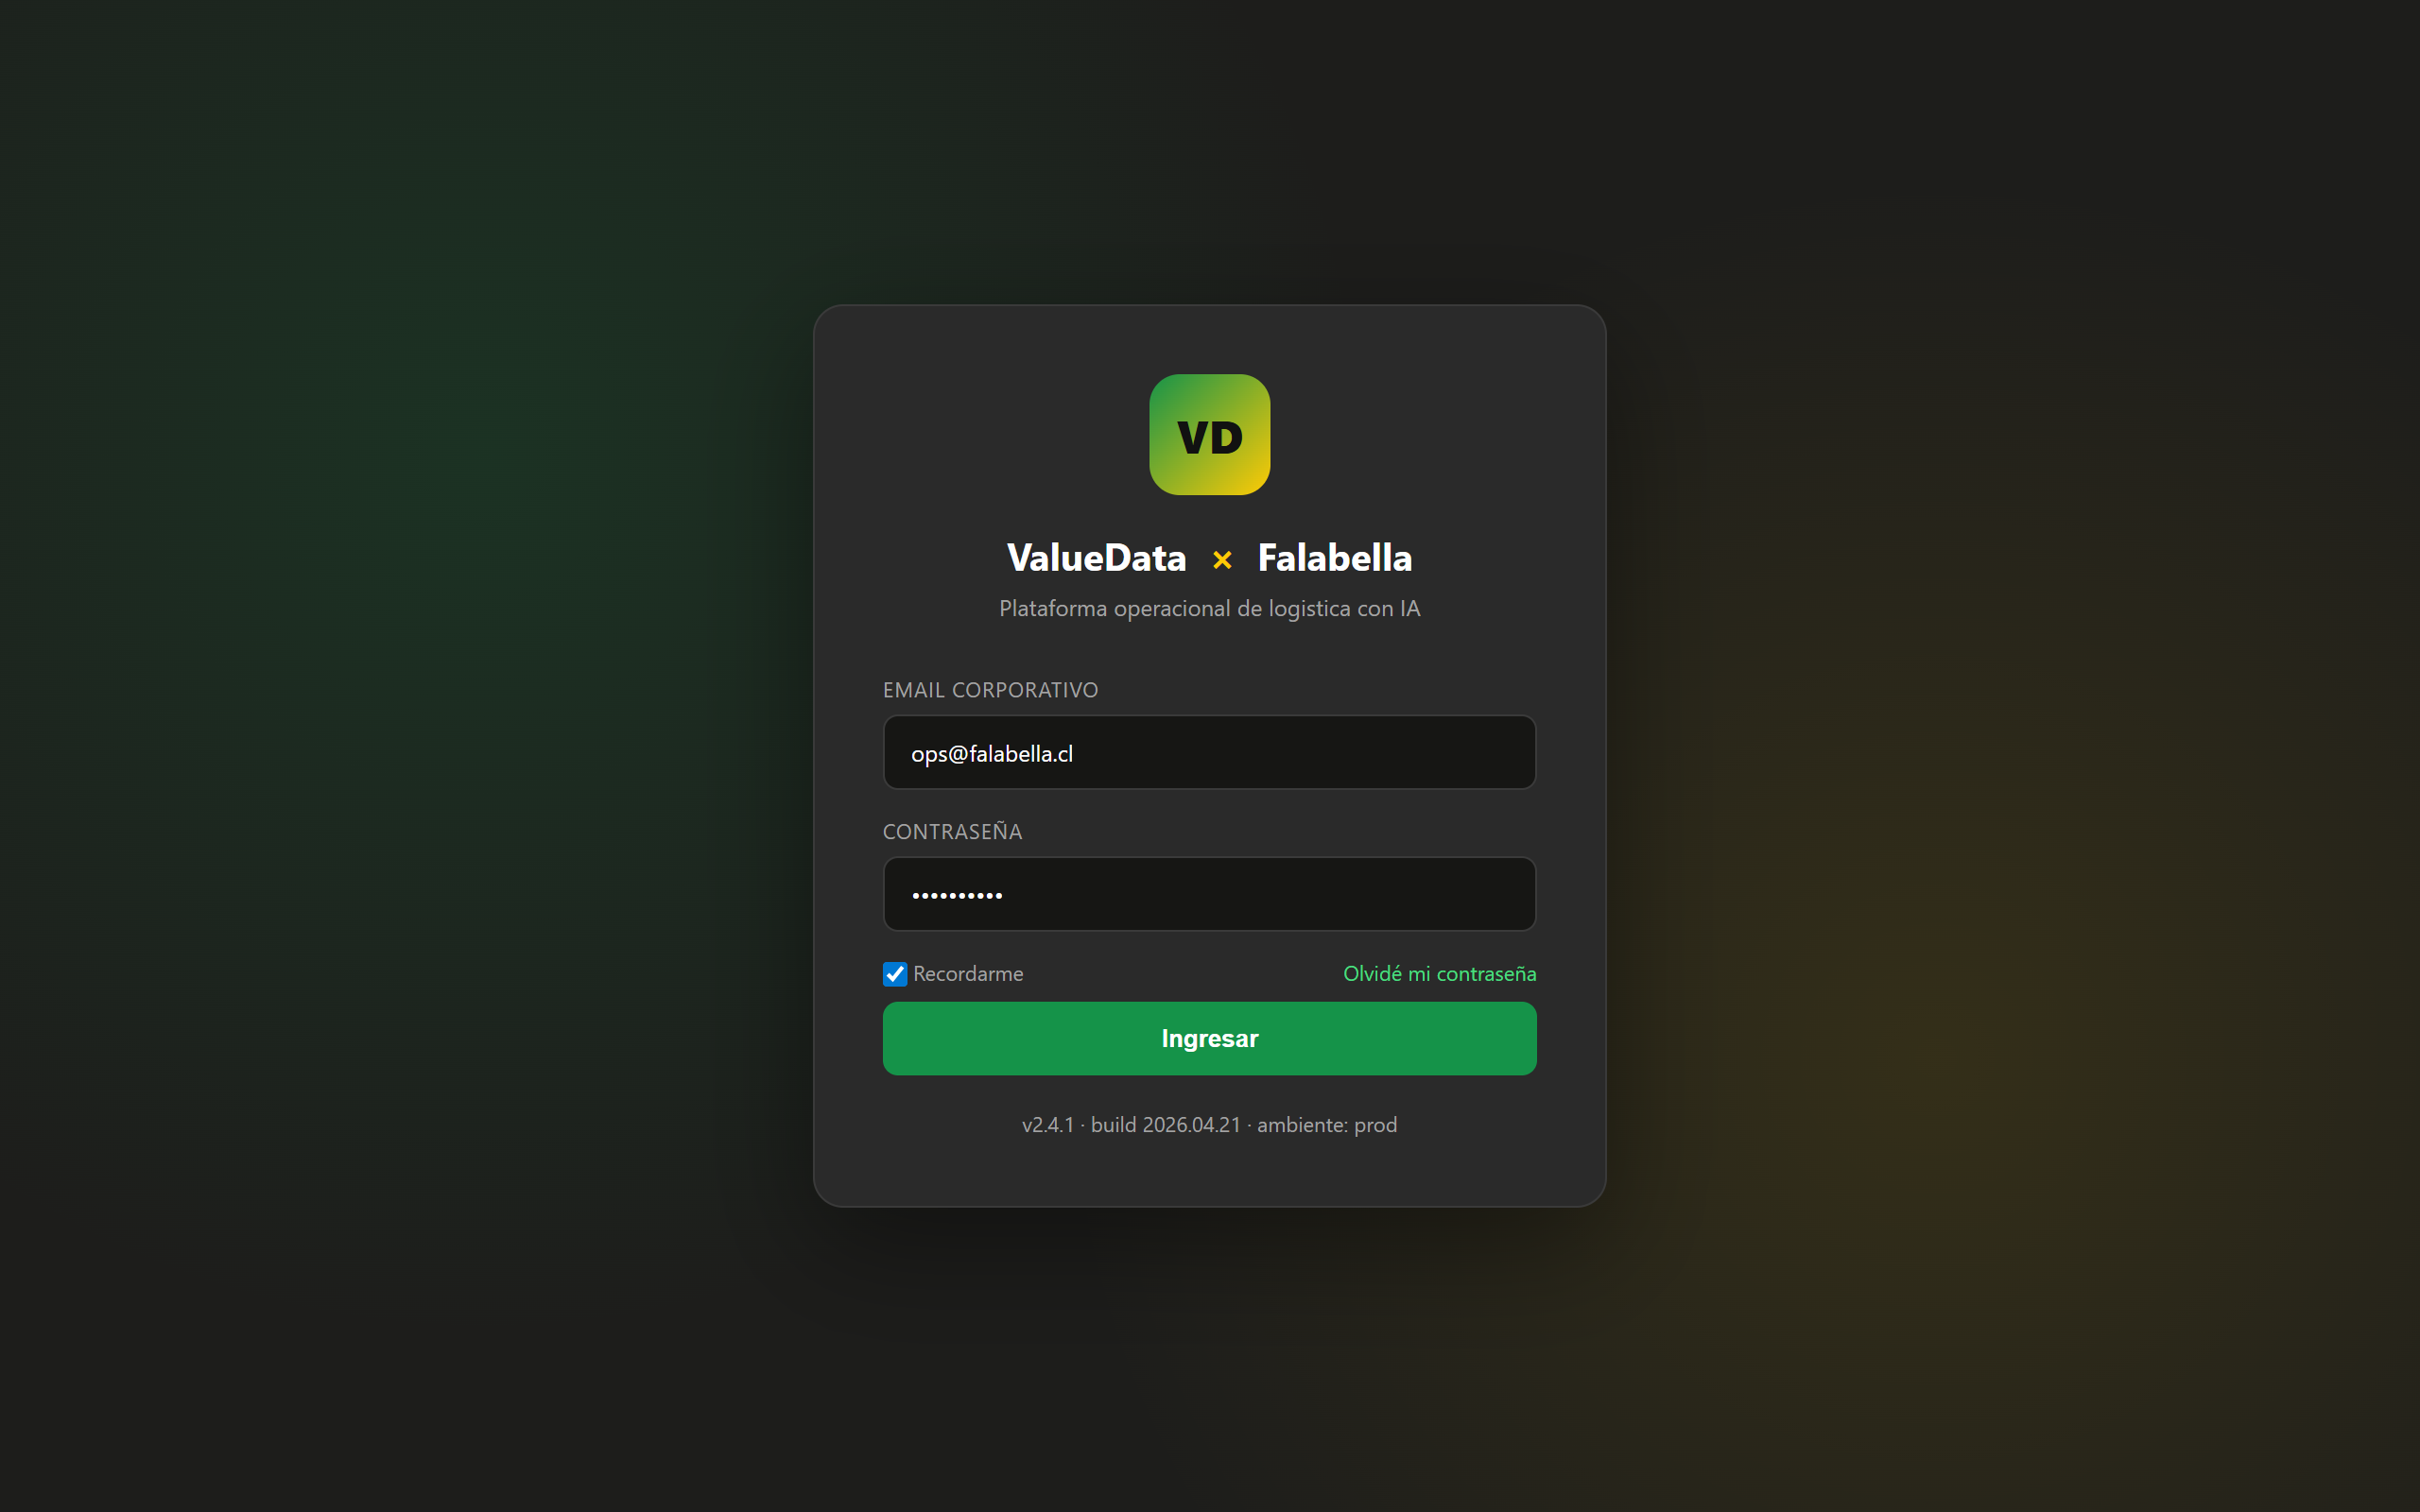
\includegraphics[width=0.85\textwidth]{01_login.png}
\caption{Pantalla de login: logo ValueData $\times$ Falabella, campos de email y contrasena, boton verde Ingresar.}
\end{figure}

La aplicacion corre en el navegador. No hay nada que instalar. Pasos:

\begin{enumerate}
  \item Abre tu navegador (Chrome, Edge o Firefox actualizado).
  \item Visita \url{https://flogging-purposely-antonym.ngrok-free.dev/}
  \item Si el navegador muestra una advertencia ngrok (es un tunel
        publico de pruebas), haz clic en \textit{``Visit Site''} para
        continuar.
  \item Veras la pantalla de \textbf{Login}: campo email, campo password,
        boton ``Ingresar''.
\end{enumerate}

\importantbox{La URL termina en \texttt{ngrok-free.dev} porque estamos
en POC. Para produccion se reemplazara por el dominio definitivo
(por ejemplo \texttt{valuedata.falabella.com}). Las credenciales y los
flujos descritos en este manual no cambian.}

\subsection{Credenciales y roles}

El POC trae cargados tres tipos de usuario para validar todos los
flujos. Solicita la password real al equipo de soporte; los valores
por defecto solo aplican al ambiente de demo:

\begin{longtable}{p{4.5cm} p{2.4cm} p{6.5cm}}
\toprule
\textbf{Email} & \textbf{Password} & \textbf{Rol y alcance} \\
\midrule
\endhead
\texttt{admin@falabella.cl}     & \texttt{admin123} &
  \textbf{falabella\_admin} --- ve todo, edita maestros, controla el dia
  simulado, configura motivos, crea VIPs y usuarios. \\
\texttt{ops@falabella.cl}       & \texttt{ops123}   &
  \textbf{falabella\_ops} --- ve todo y opera, pero no puede crear
  usuarios ni resetear el dia. \\
\texttt{transporte01@demo.cl}   & \texttt{demo123}  &
  \textbf{transport\_manager} de la empresa transportista \#1. Ve solo
  los vehiculos, drivers y visitas de su propia empresa. \\
\texttt{transporte02@demo.cl}   & \texttt{demo123}  &
  Manager de la empresa \#2. \\
\texttt{transporte03@demo.cl}   & \texttt{demo123}  &
  Manager de la empresa \#3. \\
\bottomrule
\end{longtable}

\warnbox{Para produccion, el equipo de Falabella define las passwords
finales y la integracion con SSO/AD. Las passwords se almacenan con
hash \texttt{bcrypt}; el sistema nunca las guarda en texto plano.}

\subsection{Cerrar sesion}

\begin{enumerate}
  \item En la barra lateral izquierda (sidebar), busca tu nombre y rol
        en la parte inferior.
  \item Haz clic en el icono de \textbf{salida} (flecha hacia la
        derecha, color rojo al hacer hover).
  \item Volveras a la pantalla de Login.
\end{enumerate}

La sesion tambien expira automaticamente despues de varias horas de
inactividad y debes volver a ingresar.

% =============================================================================
\section{Roles y permisos}
% =============================================================================

La plataforma distingue tres roles con visibilidad y permisos
distintos. Lo que cada rol ve esta determinado por el backend, no por
la UI: aunque alguien adivinara una URL, el backend devuelve 403 si no
corresponde.

\subsection{Falabella Admin}

\textbf{Quien:} responsable global de la operacion logistica de
Falabella, area de control de torre.

\textbf{Que ve:} \textit{todo}. Visitas y vehiculos de todas las
empresas transportistas, todos los contactos, todos los VIPs.

\textbf{Que puede hacer:}
\begin{itemize}
  \item Crear / editar / desactivar empresas transportistas.
  \item Cargar contactos en bulk (CSV) y marcar opt-ins WhatsApp.
  \item Configurar el catalogo de motivos: cuales son alertables, su
        severidad, su descripcion operacional (que llega como prompt
        al LLM).
  \item Crear, editar y desactivar clientes VIP, configurar la hora
        limite de cada uno.
  \item Crear usuarios login (otros admins, ops, managers).
  \item Configurar el dia: regenerar el plan, cambiar el reloj
        simulado, activar/pausar el avance automatico.
  \item Aceptar / rechazar / archivar correcciones de motivo
        sugeridas por la IA.
\end{itemize}

\subsection{Falabella Operaciones}

\textbf{Quien:} despachador de torre, analista de operaciones del dia.

\textbf{Que ve:} igual que el admin --- todas las empresas y visitas.

\textbf{Que puede hacer:} casi todo lo del admin, \textbf{salvo}:
\begin{itemize}
  \item Crear / borrar usuarios login (es exclusivo del admin).
  \item Resetear el dia simulado o cambiar el reloj.
\end{itemize}

Tipicamente, el rol Ops esta enfocado en monitorear la operacion en
vivo, gestionar alertas y validar las sugerencias de la IA.

\subsection{Manager Transportista}

\textbf{Quien:} jefe de operaciones / coordinador de una empresa
transportista (Transporte 01, 02, 03 \dots).

\textbf{Que ve:} \textit{solo lo de su empresa}. El backend filtra
todas las consultas de visitas, vehiculos, drivers, contactos, etc.
por \texttt{empresa\_id}.

\textbf{Que puede hacer:}
\begin{itemize}
  \item Ver el plan del dia con sus rutas y visitas.
  \item Ver el watchlist con sus visitas en riesgo.
  \item Comentar visitas (reportar motivos de no-entrega).
  \item Ver los KPIs y el scorecard de sus drivers.
\end{itemize}

\textbf{Que NO puede hacer:}
\begin{itemize}
  \item Ver visitas o drivers de otra empresa transportista.
  \item Editar el catalogo de motivos.
  \item Gestionar VIPs.
  \item Aceptar / rechazar correcciones de motivo (las dispara el
        admin/ops Falabella).
\end{itemize}

% =============================================================================
\section{Recorrido general de la pantalla}
% =============================================================================

\subsection{Sidebar (6 modulos)}

\begin{figure}[H]
\centering
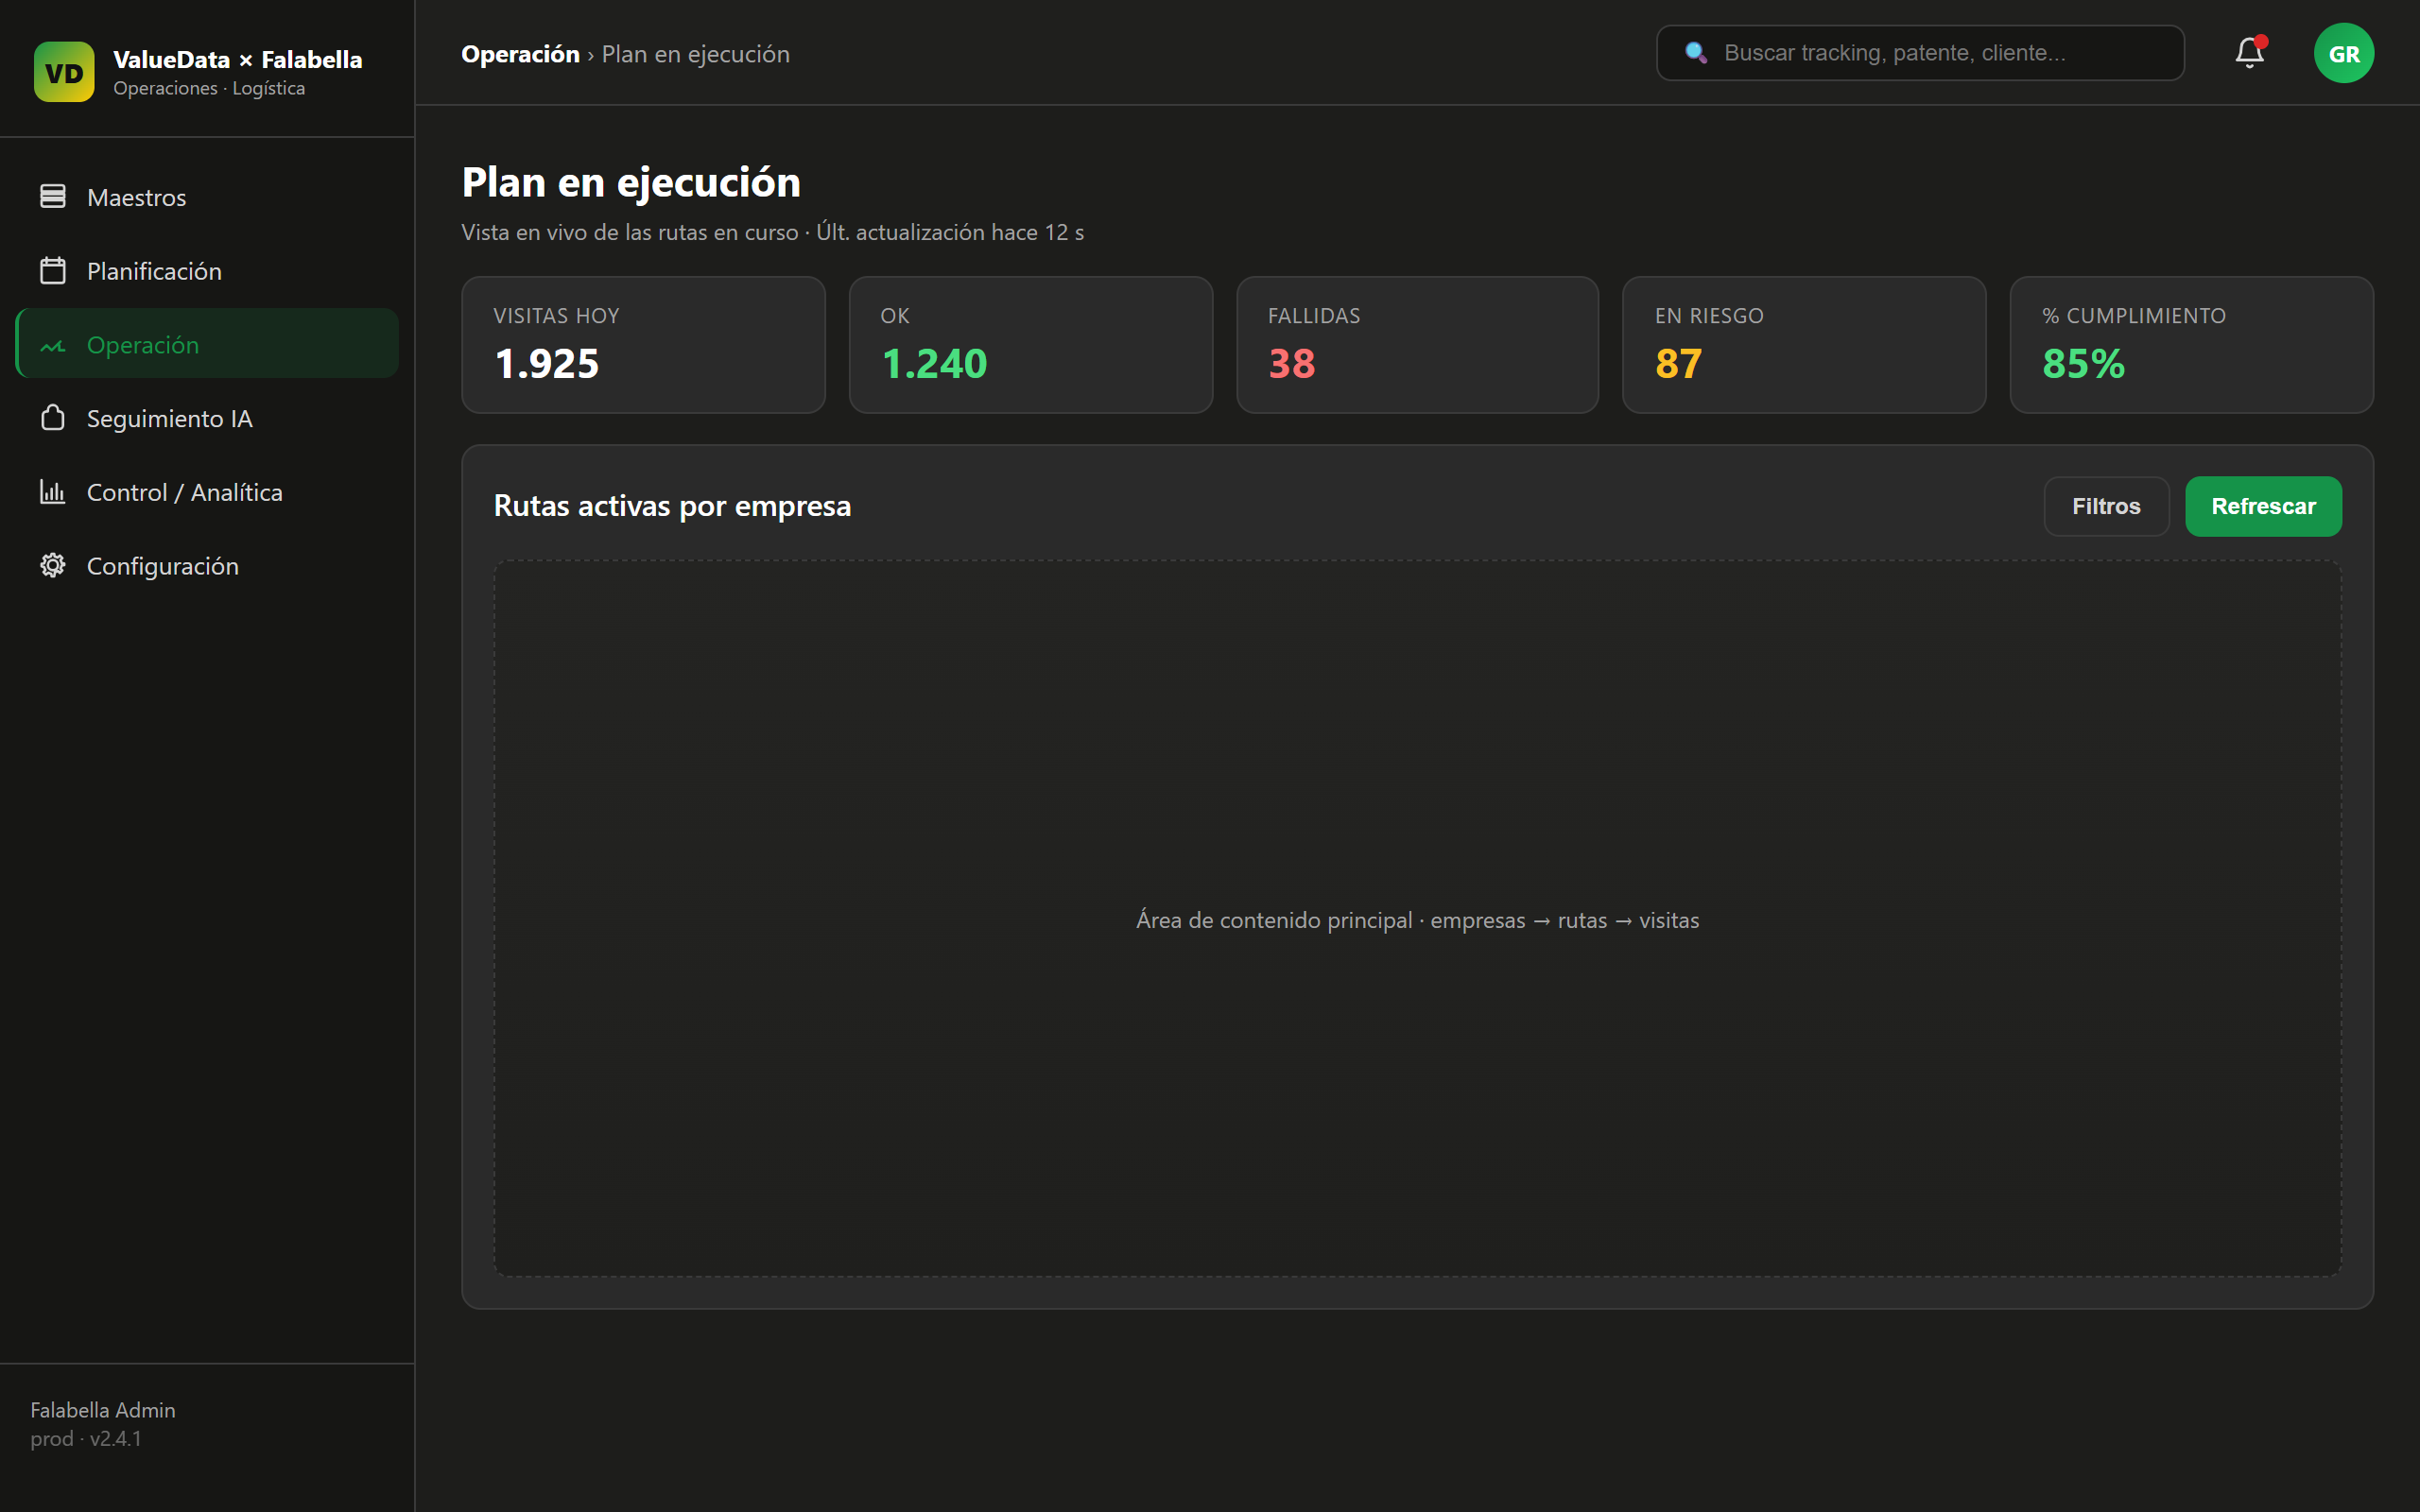
\includegraphics[width=0.95\textwidth]{02_sidebar_overview.png}
\caption{Vista general de la app: sidebar con los 6 modulos, topbar con breadcrumb, buscador, campana de notificaciones y avatar. El area central muestra el contenido del modulo activo (en este caso Plan en ejecucion).}
\end{figure}

A la izquierda, el sidebar agrupa los seis modulos en cuatro
secciones tematicas. Estan separadas por una linea sutil:

\begin{longtable}{p{2.6cm} p{2.6cm} p{8.2cm}}
\toprule
\textbf{Grupo} & \textbf{Modulo} & \textbf{Que contiene} \\
\midrule
\endhead
Datos
  & Maestros
  & Empresas, contactos, vehiculos, drivers, VIPs, usuarios, motivos. \\
Operaciones
  & Planificacion
  & Carga de entregas, plan del dia (preparacion), config dia. \\
Operaciones
  & Operacion
  & Plan en ejecucion, watchlist, mapa, alertas en vivo. \\
Analitica
  & Seguimiento IA
  & Comentarios recientes, asistente IA, correcciones de motivo. \\
Analitica
  & Control / Analitica
  & KPIs, driver scorecard, notificaciones log, modelo XGBoost. \\
Sistema
  & Configuracion
  & Alertas globales, WhatsApp/Twilio, LLM, integraciones. \\
\bottomrule
\end{longtable}

El sidebar puede colapsarse con la flecha del fondo: en modo colapsado
solo se ven los iconos. El estado se persiste en el navegador para que
la siguiente vez recuerdes tu preferencia.

\subsection{Topbar (breadcrumb, buscador, notificaciones, perfil)}

La barra superior tiene cuatro elementos, de izquierda a derecha:

\begin{enumerate}
  \item \textbf{Breadcrumb:} muestra ``Modulo / Sub-tab'' (ej.
        ``Maestros / Empresas y contactos''). Te indica donde estas.
  \item \textbf{Buscador global:} centro, ancho fijo. Busca empresas,
        contactos, drivers, visitas, VIPs y motivos en simultaneo.
  \item \textbf{Campana de notificaciones:} icono de campana arriba a
        la derecha. Muestra los 10 eventos mas recientes; un punto
        rojo indica cuantos no leiste. Refresca cada 5 segundos.
  \item \textbf{Perfil del usuario:} en la parte inferior del sidebar,
        no del topbar (en este POC). Muestra inicial, nombre, rol /
        empresa y boton de cerrar sesion.
\end{enumerate}

\subsection{Buscador global (como usarlo)}

\begin{enumerate}
  \item Haz clic en el campo \emph{``Buscar empresa, contacto, driver,
        visita, VIP, motivo\dots''} en la topbar (o presiona
        \texttt{Ctrl+K} en teclados estandar, si el atajo esta
        habilitado).
  \item Escribe al menos \textbf{2 caracteres}. La busqueda se dispara
        con un debounce de 300\,ms.
  \item Aparece un dropdown segmentado por categorias: Empresas,
        Contactos, Drivers, Visitas, VIPs, Motivos. Cada seccion muestra
        un contador a la derecha.
  \item Navega con \textbf{flecha arriba/abajo} y selecciona con
        \textbf{Enter}, o haz clic directo.
  \item Al seleccionar, la app te lleva al modulo correspondiente y
        resalta el item buscado (la fila se marca con un borde).
  \item \texttt{Esc} cierra el dropdown y limpia el termino.
\end{enumerate}

\tipbox{Para encontrar rapido un tracking, escribe los ultimos 4 a 6
caracteres del \texttt{tracking\_id}. Para encontrar un cliente VIP por
razon social, escribe parte del nombre.}

% =============================================================================
\section{Modulo MAESTROS}
% =============================================================================

\textit{Acceso:} Sidebar $\rightarrow$ Maestros. Sub-tabs disponibles
para Falabella admin/ops: Empresas y contactos, Vehiculos, Drivers,
Clientes VIP, Usuarios, Catalogo motivos. El manager transportista solo
ve la sub-tab \emph{Empresas y contactos} (filtrada a su propia
empresa).

\subsection{Empresas y contactos}

\begin{figure}[H]
\centering
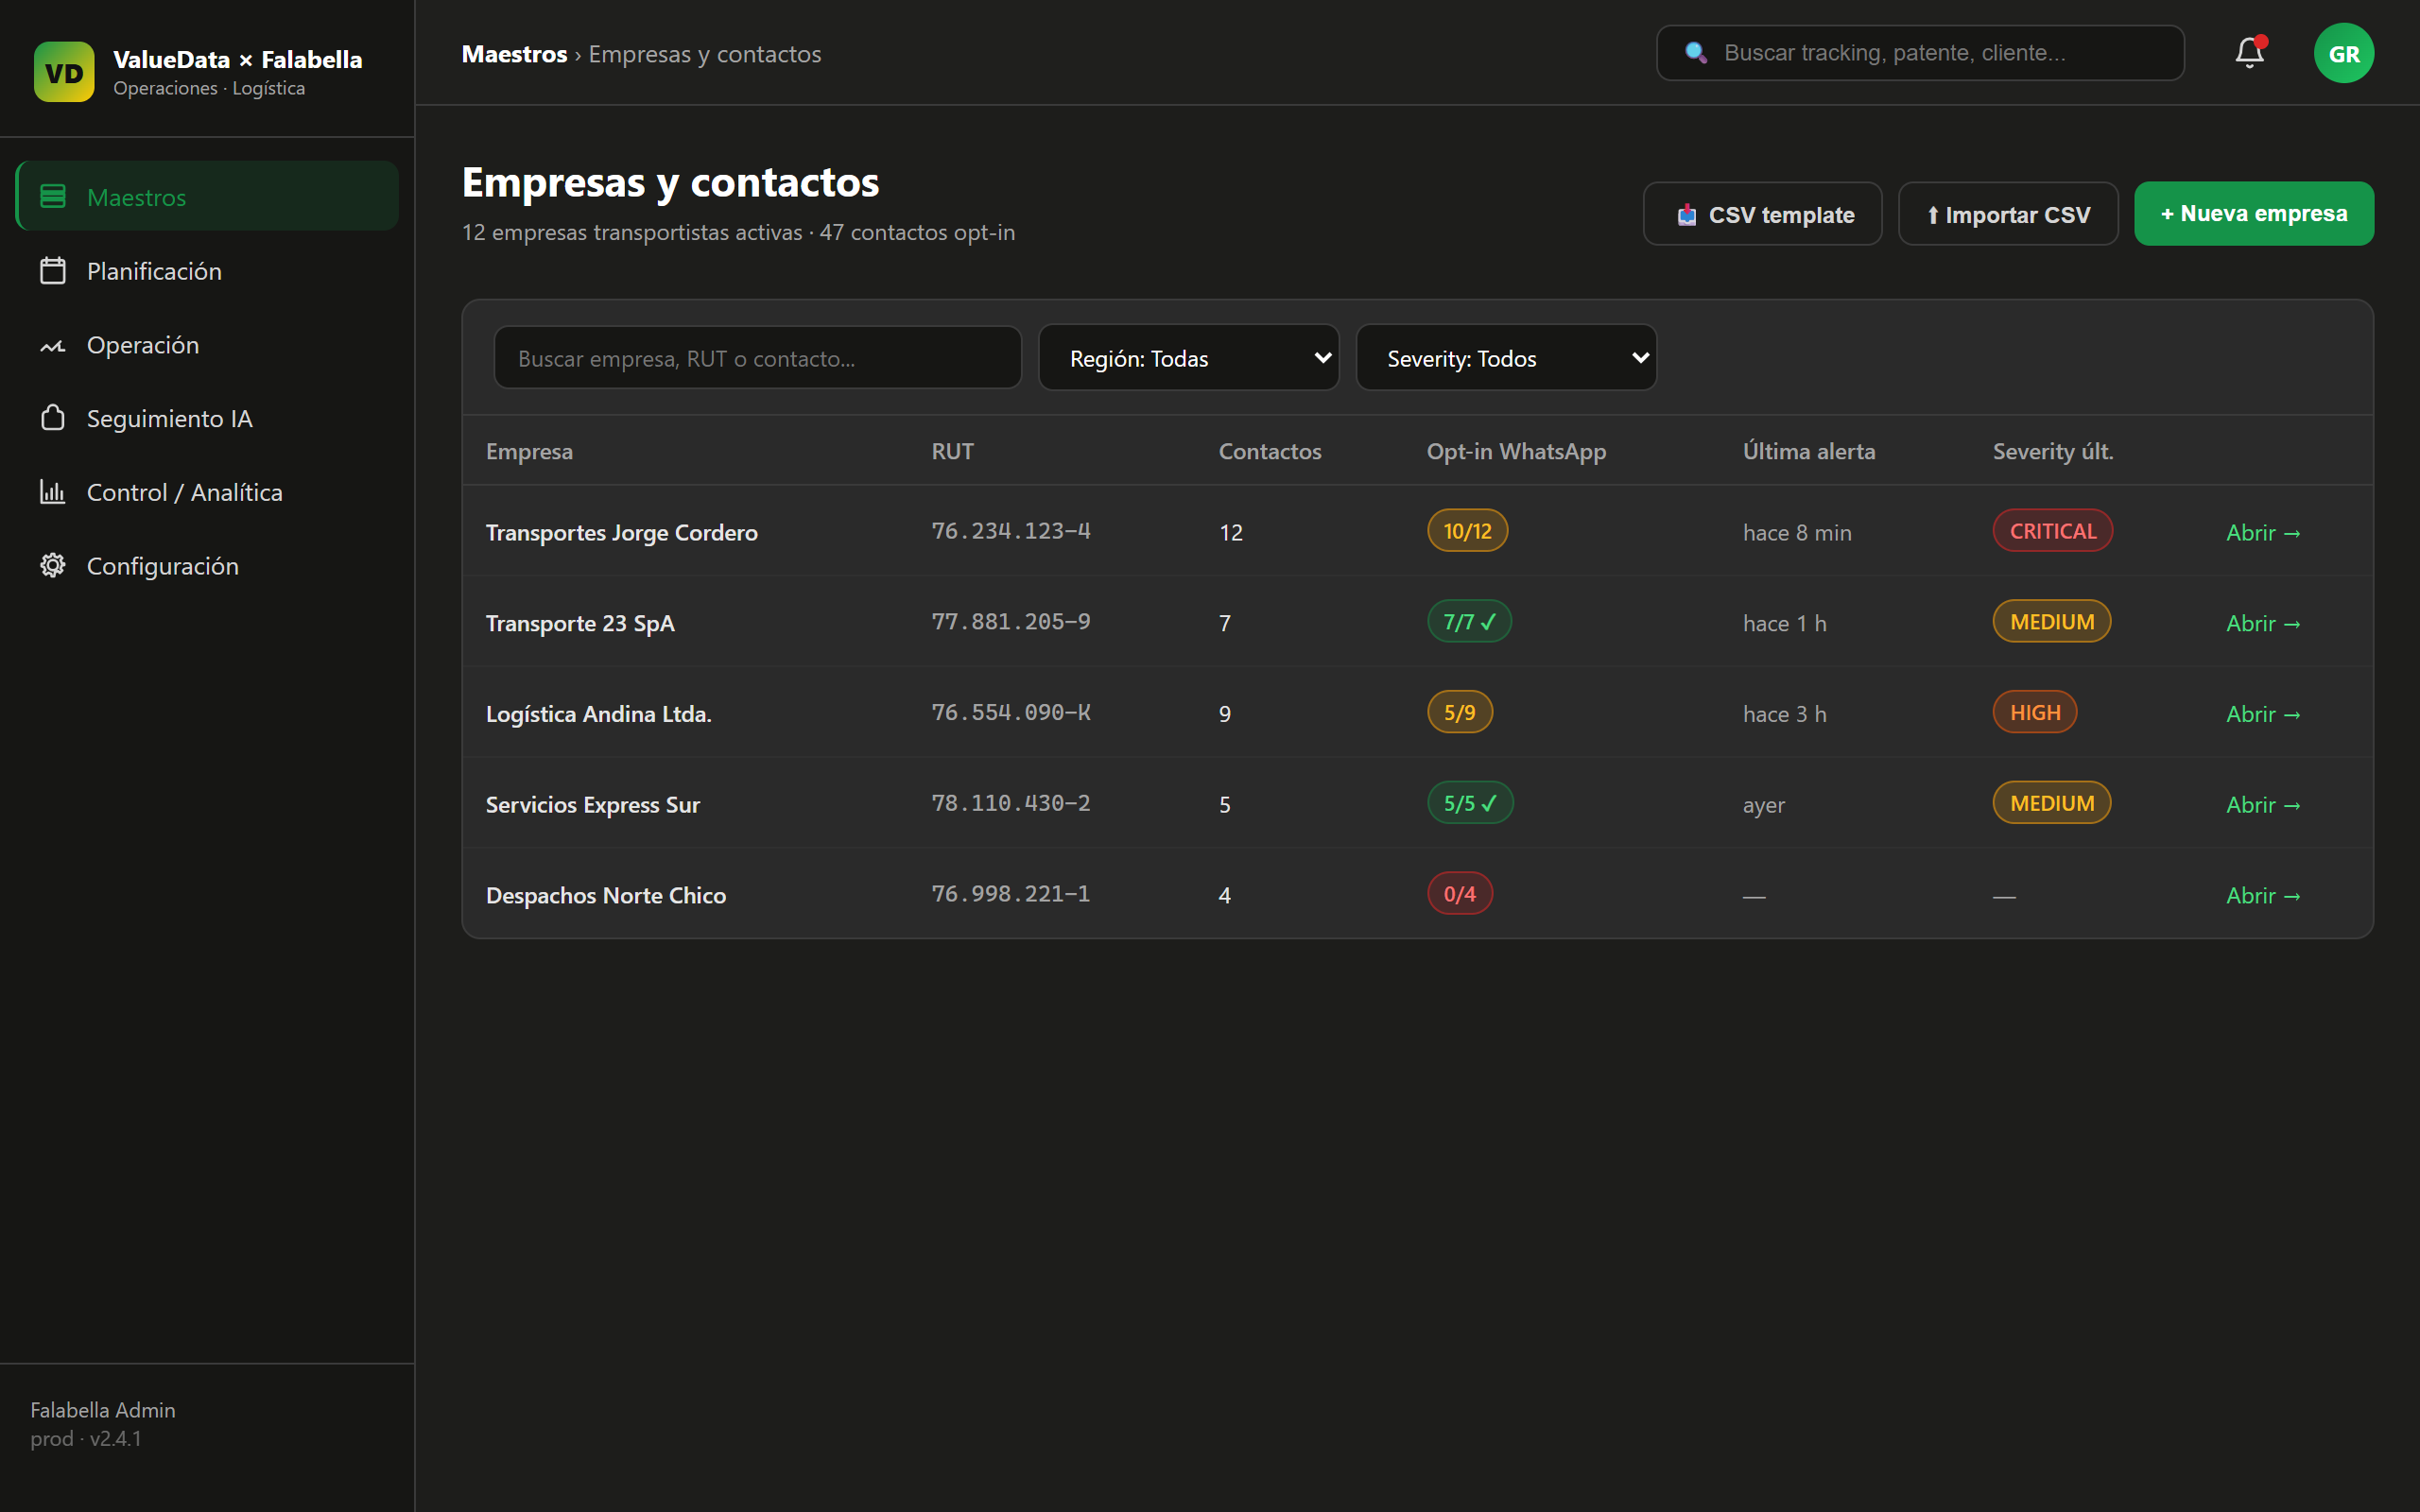
\includegraphics[width=0.95\textwidth]{03_maestros_empresas.png}
\caption{Listado de empresas transportistas: tabla con RUT, contactos, opt-in WhatsApp, severity de la ultima alerta. Boton CSV template arriba a la derecha.}
\end{figure}

\begin{figure}[H]
\centering
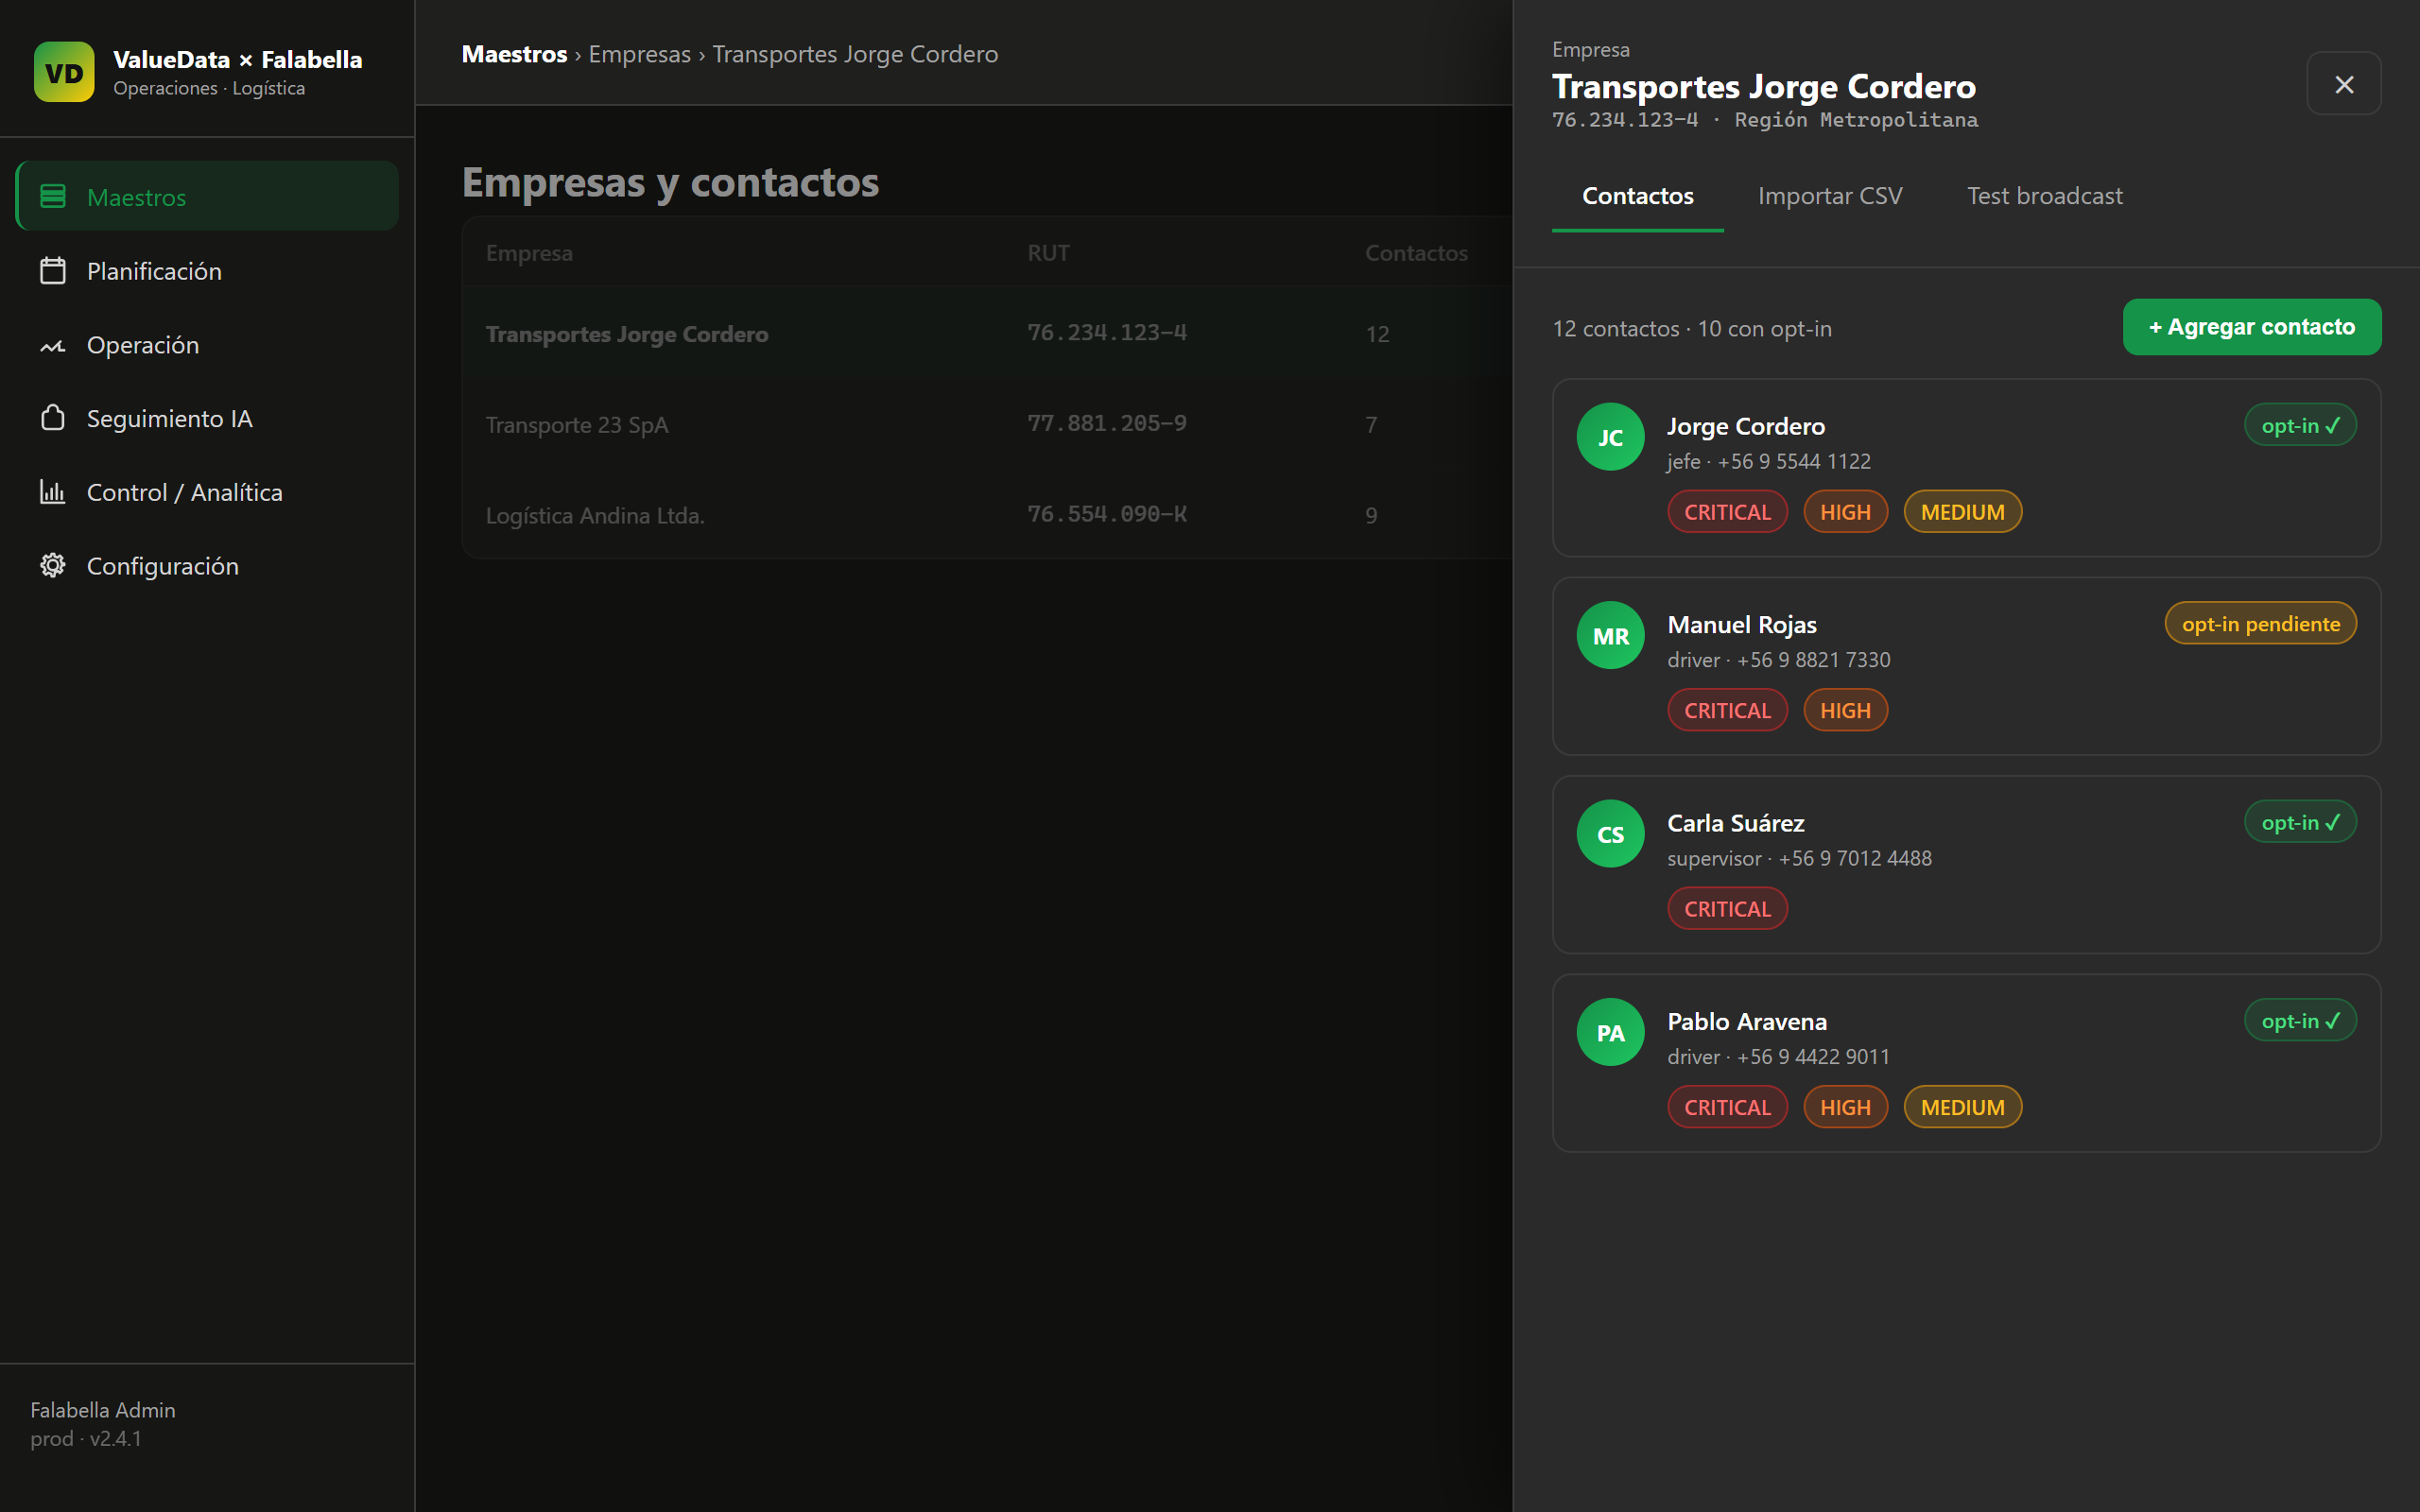
\includegraphics[width=0.95\textwidth]{04_empresa_drawer.png}
\caption{Drawer lateral de una empresa: tabs Contactos, Importar CSV y Test broadcast. La tab Contactos lista cada persona con telefono, severidades habilitadas y estado de opt-in.}
\end{figure}

Esta sub-tab es la mas importante del modulo. Aqui se decide quien
recibe los WhatsApp de alerta. Un \textbf{contacto} no necesita tener
cuenta para recibir alertas: basta con que tenga numero E.164 valido y
opt-in.

\subsubsection{Crear empresa}

\textit{Solo Admin Falabella.} Las empresas se gestionan en una
sub-pantalla. Para crear una nueva:

\begin{enumerate}
  \item Sidebar $\rightarrow$ Maestros $\rightarrow$ Empresas y
        contactos. Si la lista de empresas ya esta visible, salta al
        paso 3.
  \item Si la empresa no aparece en la tabla principal, ve a la sub-tab
        \emph{Empresas} (cuando esta disponible) o llama al endpoint
        admin (\texttt{POST /api/admin/empresas}). En el flujo del POC
        las tres empresas (\#1, \#2, \#3) ya estan creadas por seed.
  \item Una empresa se identifica por \texttt{empresa\_id} y nombre.
        Al crearla queda \emph{Activa} por defecto.
\end{enumerate}

\subsubsection{Agregar contactos manualmente}

\begin{enumerate}
  \item En la tabla principal de empresas, haz clic en
        \emph{``Ver contactos $\rightarrow$''} de la fila deseada.
  \item Se abre un \textbf{drawer lateral} con tres pestanas:
        Contactos, Importar CSV, Test broadcast.
  \item En \emph{Contactos}, haz clic en \textbf{``+ Agregar contacto''}.
  \item Completa el formulario:
    \begin{itemize}
      \item \textbf{Nombre:} obligatorio.
      \item \textbf{Rol:} jefe, coordinador, dispatcher, driver, otro.
      \item \textbf{Telefono E.164:} formato internacional. Debe
            empezar por \texttt{+}, seguido de 8 a 15 digitos.
            Ejemplo: \texttt{+56939568904}. La UI valida el formato y
            marca el campo en rojo si esta mal.
      \item \textbf{Email:} opcional.
      \item \textbf{Severidades:} chips multi-seleccion (low, medium,
            high, critical). Vacio = recibe todas las severidades.
      \item \textbf{Motivos:} chips multi-seleccion sobre los 13 del
            catalogo. Vacio = recibe todos los motivos.
      \item \textbf{Region:} radio buttons --- Solo RM, Solo regiones,
            Todas. Filtra que alertas le llegan segun donde ocurra la
            visita.
      \item \textbf{Notas:} texto libre.
    \end{itemize}
  \item Haz clic en \textbf{Guardar}. El contacto aparece en la lista
        con estado \emph{pendiente} (aun sin opt-in WhatsApp).
\end{enumerate}

\subsubsection{Importar contactos por CSV (con plantilla)}

Util para alta masiva al inicio del proyecto.

\begin{enumerate}
  \item En el drawer de la empresa, ve a la pestana \emph{Importar CSV}.
  \item Haz clic en \textbf{``Descargar template''}. Se descarga un
        archivo con el header esperado:\\
        \texttt{nombre, rol, phone\_e164, email, severities, motivos,
        region}.
  \item Llena el archivo en Excel / Google Sheets. Reglas:
    \begin{itemize}
      \item \texttt{phone\_e164} debe ser E.164 valido (ver arriba).
      \item \texttt{severities} y \texttt{motivos} se separan por
            \texttt{;} (punto y coma) dentro de la celda. Ejemplo:
            \texttt{high;critical}.
      \item \texttt{region} es \texttt{RM}, \texttt{regiones} o
            \texttt{all}.
      \item Filas con phone duplicado en la empresa se saltan
            silenciosamente.
      \item Filas con phone invalido se reportan al final del proceso
            con la razon del rechazo.
    \end{itemize}
  \item Guarda el archivo como CSV (separador coma, encoding UTF-8).
  \item Vuelve al drawer y haz clic en \emph{``Seleccionar archivo
        CSV''}. Elige el archivo.
  \item Haz clic en \textbf{Subir}. El backend procesa la lista y
        devuelve un resumen: cuantos creados, cuantos saltados, cuantos
        invalidos (con la razon).
  \item La lista de contactos se refresca automaticamente.
\end{enumerate}

\tipbox{Si tu plantilla viene de un Excel con encabezados en
mayusculas, no importa: el backend normaliza los headers a lowercase.}

\subsubsection{Marcar opt-in WhatsApp}

Por regulacion (Twilio, Meta, BSP), un numero solo puede recibir
mensajes despues de aceptar explicitamente. En el POC se simula con un
boton; en produccion se reemplaza por la respuesta del usuario al
mensaje de bienvenida.

\begin{enumerate}
  \item En la lista de contactos, busca uno con badge amarillo
        \emph{``pendiente''}.
  \item Haz clic en \textbf{``marcar opt-in''} (icono check verde).
  \item El badge cambia a verde \emph{``opt-in''} y queda registrado el
        timestamp \texttt{opted\_in\_at}.
  \item A partir de ese momento ese contacto recibe los WhatsApp de
        alerta que le correspondan por filtros (severidad, motivo,
        region).
\end{enumerate}

\warnbox{En produccion los opt-ins NO se marcan a mano. El usuario debe
responder afirmativamente al primer template de bienvenida que envia
Twilio. Si tu lista tiene 100 contactos pero solo 30 tienen opt-in,
solo 30 reciben alertas.}

\subsubsection{Test broadcast (mensaje de prueba)}

Permite verificar que un canal funciona sin esperar una alerta real.

\begin{enumerate}
  \item En el drawer de la empresa, pestana \emph{Test broadcast}.
  \item Escribe el cuerpo del mensaje en el campo de texto.
  \item Selecciona los destinatarios (todos los con opt-in, o un sub-set).
  \item Haz clic en \textbf{Enviar}.
  \item El backend dispara los mensajes via Twilio y muestra un resumen:
        cuantos enviados, cuantos fallaron y la razon (numero invalido,
        opt-in revocado, sandbox restringido, etc.).
\end{enumerate}

\subsection{Vehiculos}

Tab disponible para Admin Falabella. Lista todos los vehiculos
extendidos del fleet (\texttt{vehicle\_id}, nombre, patente, tipo,
ano, capacidad m\(^3\)). En este POC los vehiculos se crean al
bootstrappear la base; el alta manual es lectura solamente. Cada
vehiculo esta asignado a una empresa transportista mediante un mapping
\texttt{vehicle\_empresa}.

\wipbox{La edicion manual de vehiculos (alta y baja) es una mejora
prevista para el siguiente sprint.}

\subsection{Drivers (choferes)}

Tab disponible para Admin Falabella. Muestra la lista de choferes con
nombre, vehiculo asignado, telefono, rating. Acciones disponibles:

\subsubsection{Editar phone E.164}

\begin{enumerate}
  \item En la fila del driver, haz clic en \textbf{Editar}.
  \item Cambia el campo \texttt{phone\_e164} al numero correcto.
        Mismo formato que en contactos.
  \item Guarda.
\end{enumerate}

\subsubsection{Activar notify\_whatsapp}

Un driver puede recibir alertas \textit{de su propia empresa} si tiene
las dos condiciones: \texttt{notify\_whatsapp=1} y
\texttt{opted\_in\_at} no nulo.

\begin{enumerate}
  \item Edita el driver.
  \item Marca el checkbox \emph{Recibir WhatsApp}.
  \item Guarda. El driver no recibe nada todavia hasta el opt-in.
\end{enumerate}

\subsubsection{Confirmar opt-in}

Mismo flujo que para contactos: boton \textbf{``marcar opt-in''}
registra \texttt{opted\_in\_at}. En produccion se reemplaza por el
flujo conversacional via Twilio.

\subsection{Clientes VIP}

\begin{figure}[H]
\centering
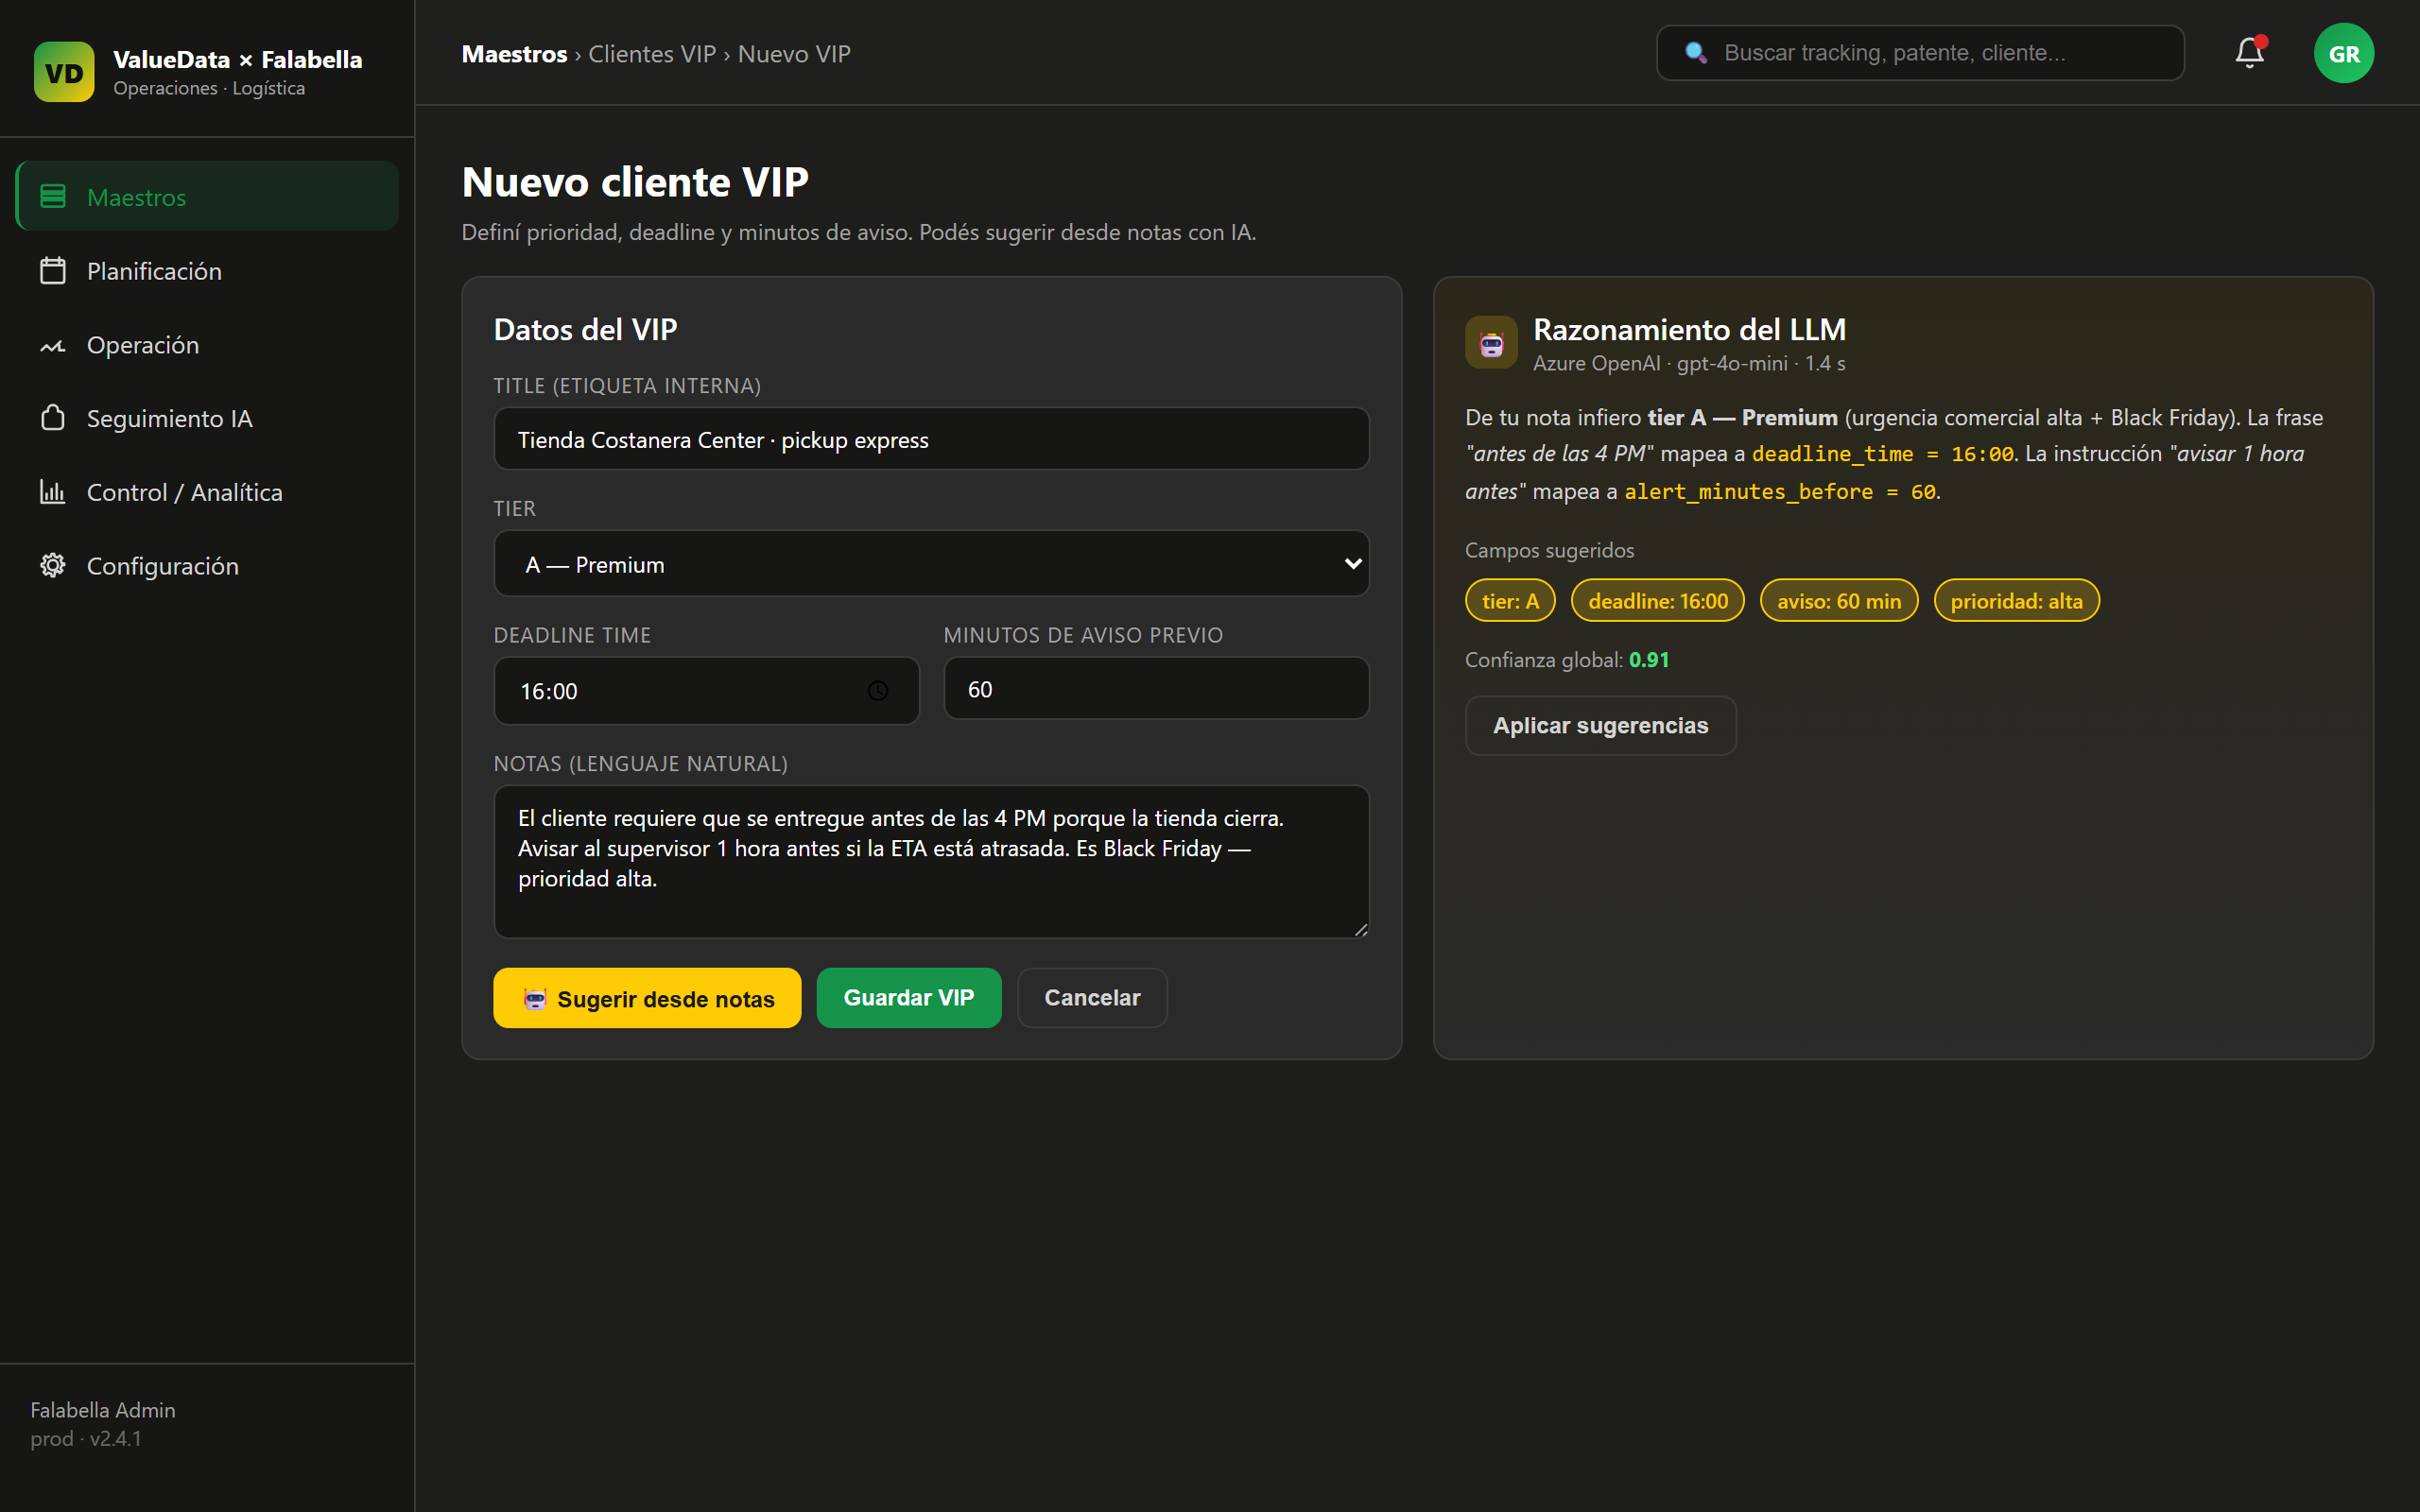
\includegraphics[width=0.95\textwidth]{05_vip_form.png}
\caption{Formulario de alta VIP: campos title, tier, deadline\_time, alert\_minutes\_before y notas en lenguaje natural. El boton amarillo Sugerir desde notas dispara al LLM, que devuelve el razonamiento y los campos sugeridos en el panel de la derecha.}
\end{figure}

Esta es una de las funcionalidades clave para Falabella: marcar
clientes que no pueden fallar y que requieren alerta anticipada cuando
estan en riesgo de no entregar antes de su hora limite.

\subsubsection{Crear VIP}

\begin{enumerate}
  \item Sidebar $\rightarrow$ Maestros $\rightarrow$ Clientes VIP.
  \item Haz clic en \textbf{``+ Nuevo VIP''}.
  \item Se abre un modal con el formulario:
    \begin{itemize}
      \item \textbf{Tipo de match:} Razon social (\texttt{title}),
            Customer ID o Referencia. Determina por cual campo se
            buscara la coincidencia con las visitas del dia.
      \item \textbf{Tier:} texto libre, por ejemplo ``VIP'',
            ``Platinum'', ``Estrategico''. Se usa para clasificar.
      \item \textbf{Valor del match (exacto):} el valor a buscar
            (ej. razon social completa). El match es exacto y
            sensible a mayusculas; copia y pega para evitar errores.
      \item \textbf{Empresa:} dropdown. Vacio = global (todas las
            transportistas), o una empresa especifica.
      \item \textbf{Notas:} texto libre. Aqui puedes describir el
            acuerdo comercial.
      \item \textbf{Hora limite (HH:MM):} hora del dia en formato 24h.
            Ejemplo: \texttt{16:00} para las 4 PM.
      \item \textbf{Alertar minutos antes (5--720):} cuantos minutos
            antes del deadline disparar la alerta. Default: 60.
      \item \textbf{Activo:} checkbox. Permite desactivar sin borrar.
    \end{itemize}
  \item Haz clic en \textbf{Crear VIP}.
\end{enumerate}

\subsubsection{Definir hora limite (deadline\_time)}

La hora limite es lo que el cron VIP usa para emitir el evento
\texttt{vip\_deadline\_warning}. Logica:

\begin{enumerate}
  \item El cron corre cada 60 segundos.
  \item Para cada VIP activo con \texttt{deadline\_time} definido,
        busca las visitas pending del dia que matcheen.
  \item Si \(now \geq (deadline - alert\_minutes\_before)\) y la VIP no
        tiene alerta enviada hoy, dispara el evento y un WhatsApp.
  \item Marca \texttt{last\_alert\_sent\_at = now} para no duplicar.
\end{enumerate}

\importantbox{La alerta VIP es independiente de los motivos de
no-entrega. Es una alerta de \emph{tiempo} (vencimiento de la
ventana). Puede convivir con alertas de motivo de la misma visita.}

\subsubsection{Boton ``Sugerir desde notas'' (IA parsea)}

Si la nota del VIP describe el acuerdo en texto libre, la IA puede
extraer la hora limite y los minutos de antelacion automaticamente:

\begin{enumerate}
  \item En el formulario VIP, escribe en \emph{Notas} algo como:
        \emph{``Cliente VIP, entregar antes de las 4 PM con 1 hora de
        aviso''}.
  \item Haz clic en \textbf{``Sugerir desde notas''} (boton con
        icono violeta de chispas).
  \item La IA analiza el texto y rellena los campos
        \texttt{deadline\_time} (16:00) y \texttt{alert\_minutes\_before}
        (60). Muestra el razonamiento abajo del boton.
  \item Si la IA falla o el texto no contiene info de hora, cae a
        un fallback de regex y lo indica con la etiqueta
        \emph{``(fallback regex)''}.
  \item Revisa los valores propuestos y ajusta si es necesario antes
        de guardar.
\end{enumerate}

\subsection{Usuarios login}

Tab disponible \textbf{solo} para Admin Falabella. Permite crear
nuevos usuarios con rol y empresa, cambiar password, desactivar.

\begin{enumerate}
  \item Sidebar $\rightarrow$ Maestros $\rightarrow$ Usuarios.
  \item Haz clic en \textbf{``+ Nuevo usuario''}.
  \item Completa email, display name, rol (\texttt{falabella\_admin},
        \texttt{falabella\_ops}, \texttt{transport\_manager}), empresa
        (solo si es transport\_manager), password.
  \item Marca el checkbox \emph{notify\_whatsapp} si el usuario debe
        recibir alertas en su numero personal (requiere opt-in).
  \item Guarda.
\end{enumerate}

Para resetear el password de un usuario existente, edita la fila e
ingresa la nueva password. El backend la hashea con bcrypt antes de
guardar.

\subsection{Catalogo de motivos}

\begin{figure}[H]
\centering
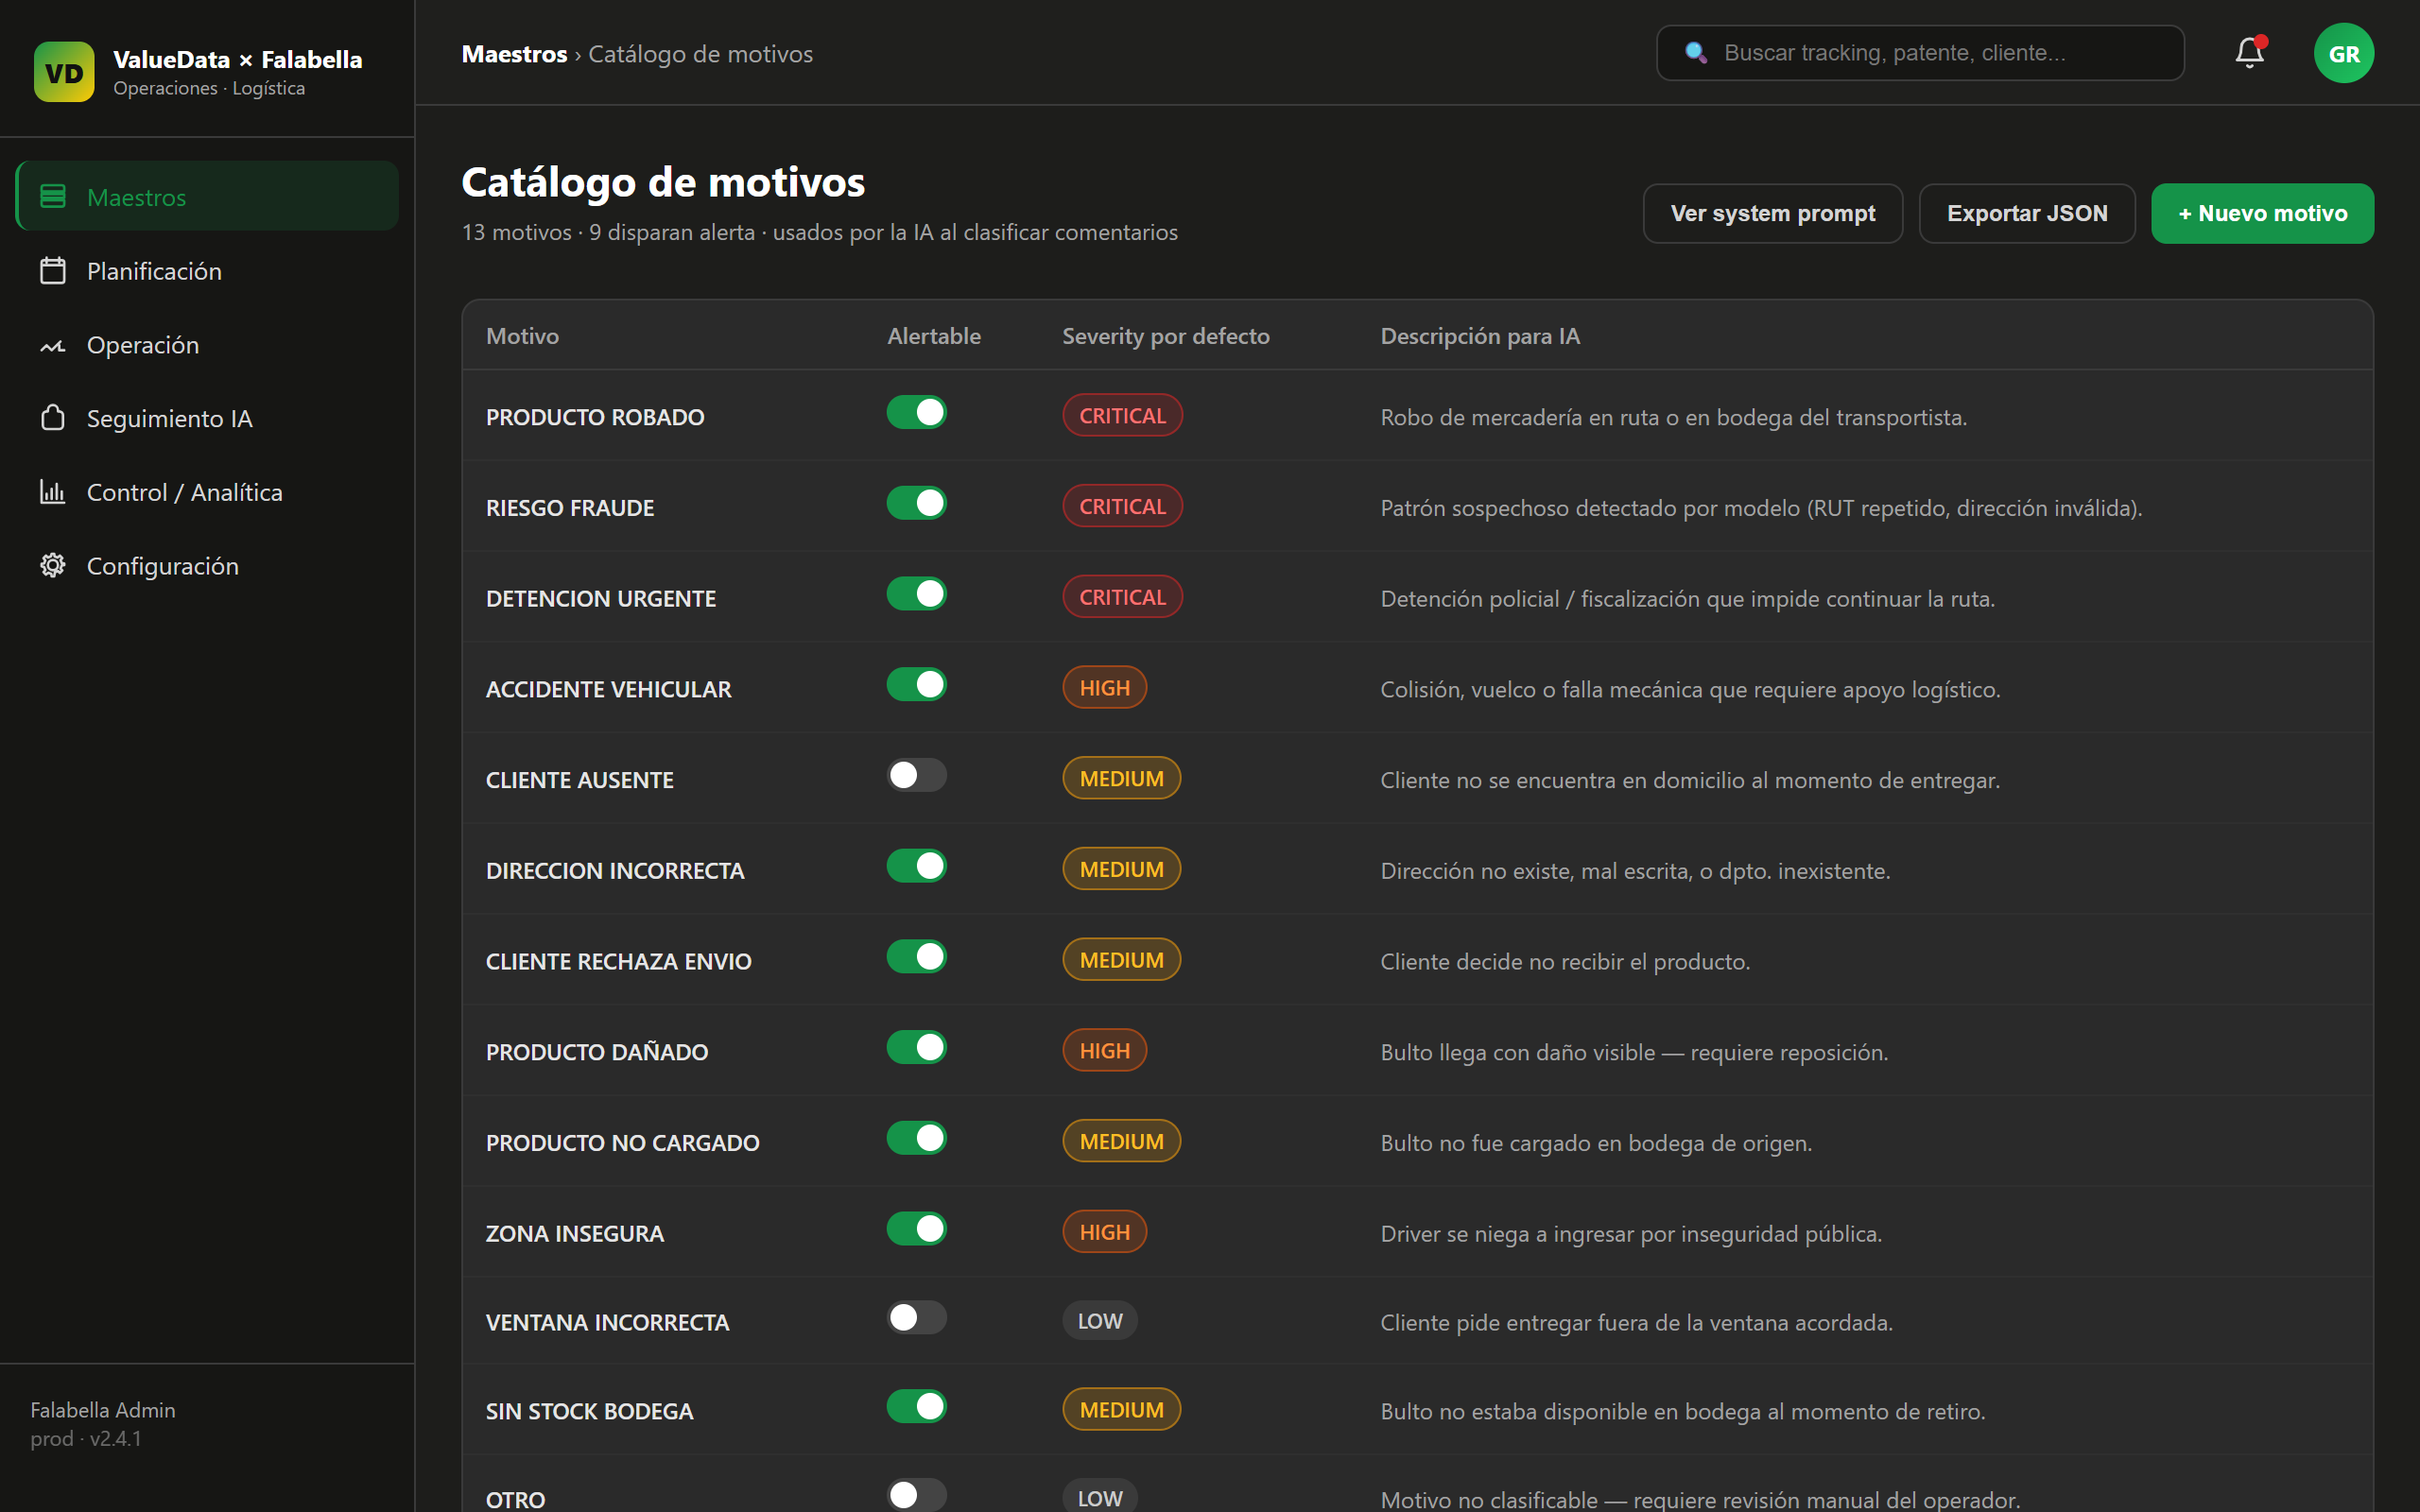
\includegraphics[width=0.95\textwidth]{06_motivos_catalogo.png}
\caption{Catalogo de los 13 motivos: toggle alertable, severity por defecto y la descripcion que consume la IA al clasificar. El boton Ver system prompt expone el prompt exacto que se envia al modelo.}
\end{figure}

Los 13 motivos del catalogo estan fijos (vienen de un notebook de
auditoria operacional de Falabella). No se pueden agregar ni borrar
desde la UI; lo que SI se puede es configurar por cada motivo:

\subsubsection{Configurar alertable / severity por empresa}

\begin{enumerate}
  \item Sidebar $\rightarrow$ Maestros $\rightarrow$ Catalogo motivos.
  \item Tabla con los 13 motivos. Columnas: Motivo, Alertable,
        Severidad, Descripcion, Ultima edicion.
  \item Haz clic en una fila para abrir el editor.
  \item Configura:
    \begin{itemize}
      \item \textbf{Alertable:} switch on/off. Si esta off, ese motivo
            no genera WhatsApp aunque el chofer lo reporte.
      \item \textbf{Severidad:} low / medium / high / critical.
      \item \textbf{Empresa:} dropdown. Vacio = global; el override
            por empresa siempre gana sobre el global.
    \end{itemize}
  \item Haz clic en \textbf{Guardar}.
\end{enumerate}

\subsubsection{Editar descripcion operacional}

La descripcion es el texto que el LLM ve cuando clasifica un comentario.
Cambiarla cambia el comportamiento del clasificador.

\begin{enumerate}
  \item En el editor, modifica el campo \emph{Descripcion}. Puedes
        usar varias lineas, listas, ejemplos.
  \item Si quieres volver al texto por defecto, haz clic en
        \textbf{``Restaurar default''}: deja el campo vacio (NULL en
        DB) y la app vuelve a usar el texto del catalogo original.
\end{enumerate}

\tipbox{La descripcion soporta el patron \emph{``NO usar si: \dots
$\rightarrow$ MOTIVO\_X''} para guiar al LLM cuando hay confusion entre
motivos similares. Por ejemplo, en SIN MORADORES: \emph{``NO usar si:
el cliente atendio pero rechazo $\rightarrow$ CLIENTE RECHAZA ENVIO''}.}

\subsubsection{Ver system prompt del LLM}

El system prompt completo que el classifier usa esta compuesto
dinamicamente con todas las descripciones. Para ver el resultado:

\begin{enumerate}
  \item Llama el endpoint \texttt{GET /api/motivos/classify/prompt}
        (curl, Postman) o usa el boton de inspeccion en la UI cuando
        este disponible.
  \item Recibiras el texto exacto que el LLM ve.
\end{enumerate}

\wipbox{El boton \emph{``Ver prompt LLM''} en la UI esta planeado para
el siguiente sprint. Por ahora se inspecciona via API.}

% =============================================================================
\section{Modulo PLANIFICACION}
% =============================================================================

Este modulo cubre todo lo que ocurre \textbf{antes} de arrancar el dia:
cargar las visitas, revisar el plan en frio, definir parametros del dia.

\subsection{Carga de entregas}

\begin{enumerate}
  \item Sidebar $\rightarrow$ Planificacion $\rightarrow$ Carga de
        entregas.
  \item Selecciona la \textbf{Fecha planificada} en el datepicker.
        Default: hoy.
  \item Haz clic en \textbf{``Importar desde SimpliRoute''}.
  \item En el POC, esto invoca un mock que devuelve el plan generado
        sinteticamente (la misma forma que tendria SimpliRoute en
        produccion).
  \item Aparece un mensaje verde con la cantidad de visitas
        importadas. La tabla \emph{Ultima carga} se actualiza con el
        registro: fecha, cantidad, origen.
\end{enumerate}

\wipbox{En produccion el boton se conecta al endpoint real de
SimpliRoute con credenciales de Falabella. La logica de matching y
enriquecimiento (CT, suborden, folios) ya esta implementada en el
backend; solo falta cambiar el stub mock por la llamada real.}

\subsection{Plan del dia (vista preparacion)}

Misma vista que en \emph{Operacion} pero en modo \textbf{planning}: sin
ETAs en vivo, sin sim\_clock, sin riesgos calculados todavia. Sirve
para revisar la asignacion de visitas a vehiculos antes del arranque.

Para detalles de la pantalla, ver Seccion 7.2 (modo \emph{live}). En
modo planning solo se omiten:
\begin{itemize}
  \item ETAs y semaforos de slack.
  \item Probabilidad de fallo.
  \item Comentarios y reportes (la visita aun no esta en la calle).
\end{itemize}

\subsection{Configuracion del dia}

\textit{Solo Admin Falabella.} Aqui se controla el reloj y el ciclo
de vida del dia simulado:

\begin{enumerate}
  \item \textbf{Congelar dia} (\texttt{POST /api/control/freeze}):
        setea el reloj a las 09:00, pausa el avance automatico. Util
        para configurar prioridades y VIPs antes de arrancar.
  \item \textbf{Arrancar dia} (\texttt{POST /api/control/start-day}):
        opcionalmente regenera el plan, mueve el reloj a 09:00 si
        estaba antes y activa el avance automatico.
  \item \textbf{Cambiar reloj} (\texttt{POST /api/control/clock}):
        avanza por offset minutos o setea una hora exacta. Usado en
        demos para saltar a la hora critica.
  \item \textbf{Reset dia} (\texttt{POST /api/control/reset}): regenera
        completamente el plan con un nuevo seed.
\end{enumerate}

\importantbox{Estas acciones existen porque el POC simula el paso del
tiempo. En produccion el reloj es el reloj real y estos controles se
deshabilitan.}

% =============================================================================
\section{Modulo OPERACION (en vivo)}
% =============================================================================

Este es el modulo central durante el dia. Cuatro sub-tabs: Plan en
ejecucion, Watchlist, Mapa, Alertas en vivo. Antes de las sub-tabs hay
una \textbf{barra de filtros globales} que aplica a todas.

\subsection{Filtros globales (region, empresa, solo VIP)}

Arriba de las sub-tabs, en gris claro:

\begin{itemize}
  \item \textbf{Region:} dropdown con \emph{Todas, Region Metropolitana,
        Todas excepto RM}, mas seleccion individual por region (Valpo,
        Biobio, Coquimbo, Maule, Araucania, OHiggins, Antofagasta).
  \item \textbf{Empresa:} dropdown con todas las empresas
        transportistas. Solo visible para Falabella admin/ops; el
        manager transportista esta forzado a su propia empresa.
  \item \textbf{Solo VIP:} checkbox. Filtra a las visitas que cruzan
        con la tabla \texttt{vip\_clients}. Pinta el icono CMR amarillo.
\end{itemize}

Debajo, una linea de \textbf{KPIs inline}: Visitas totales, OK,
Fallidas, En riesgo, \% cumplimiento. Refresca cada 10 segundos.

\subsection{Plan en ejecucion}

\begin{figure}[H]
\centering
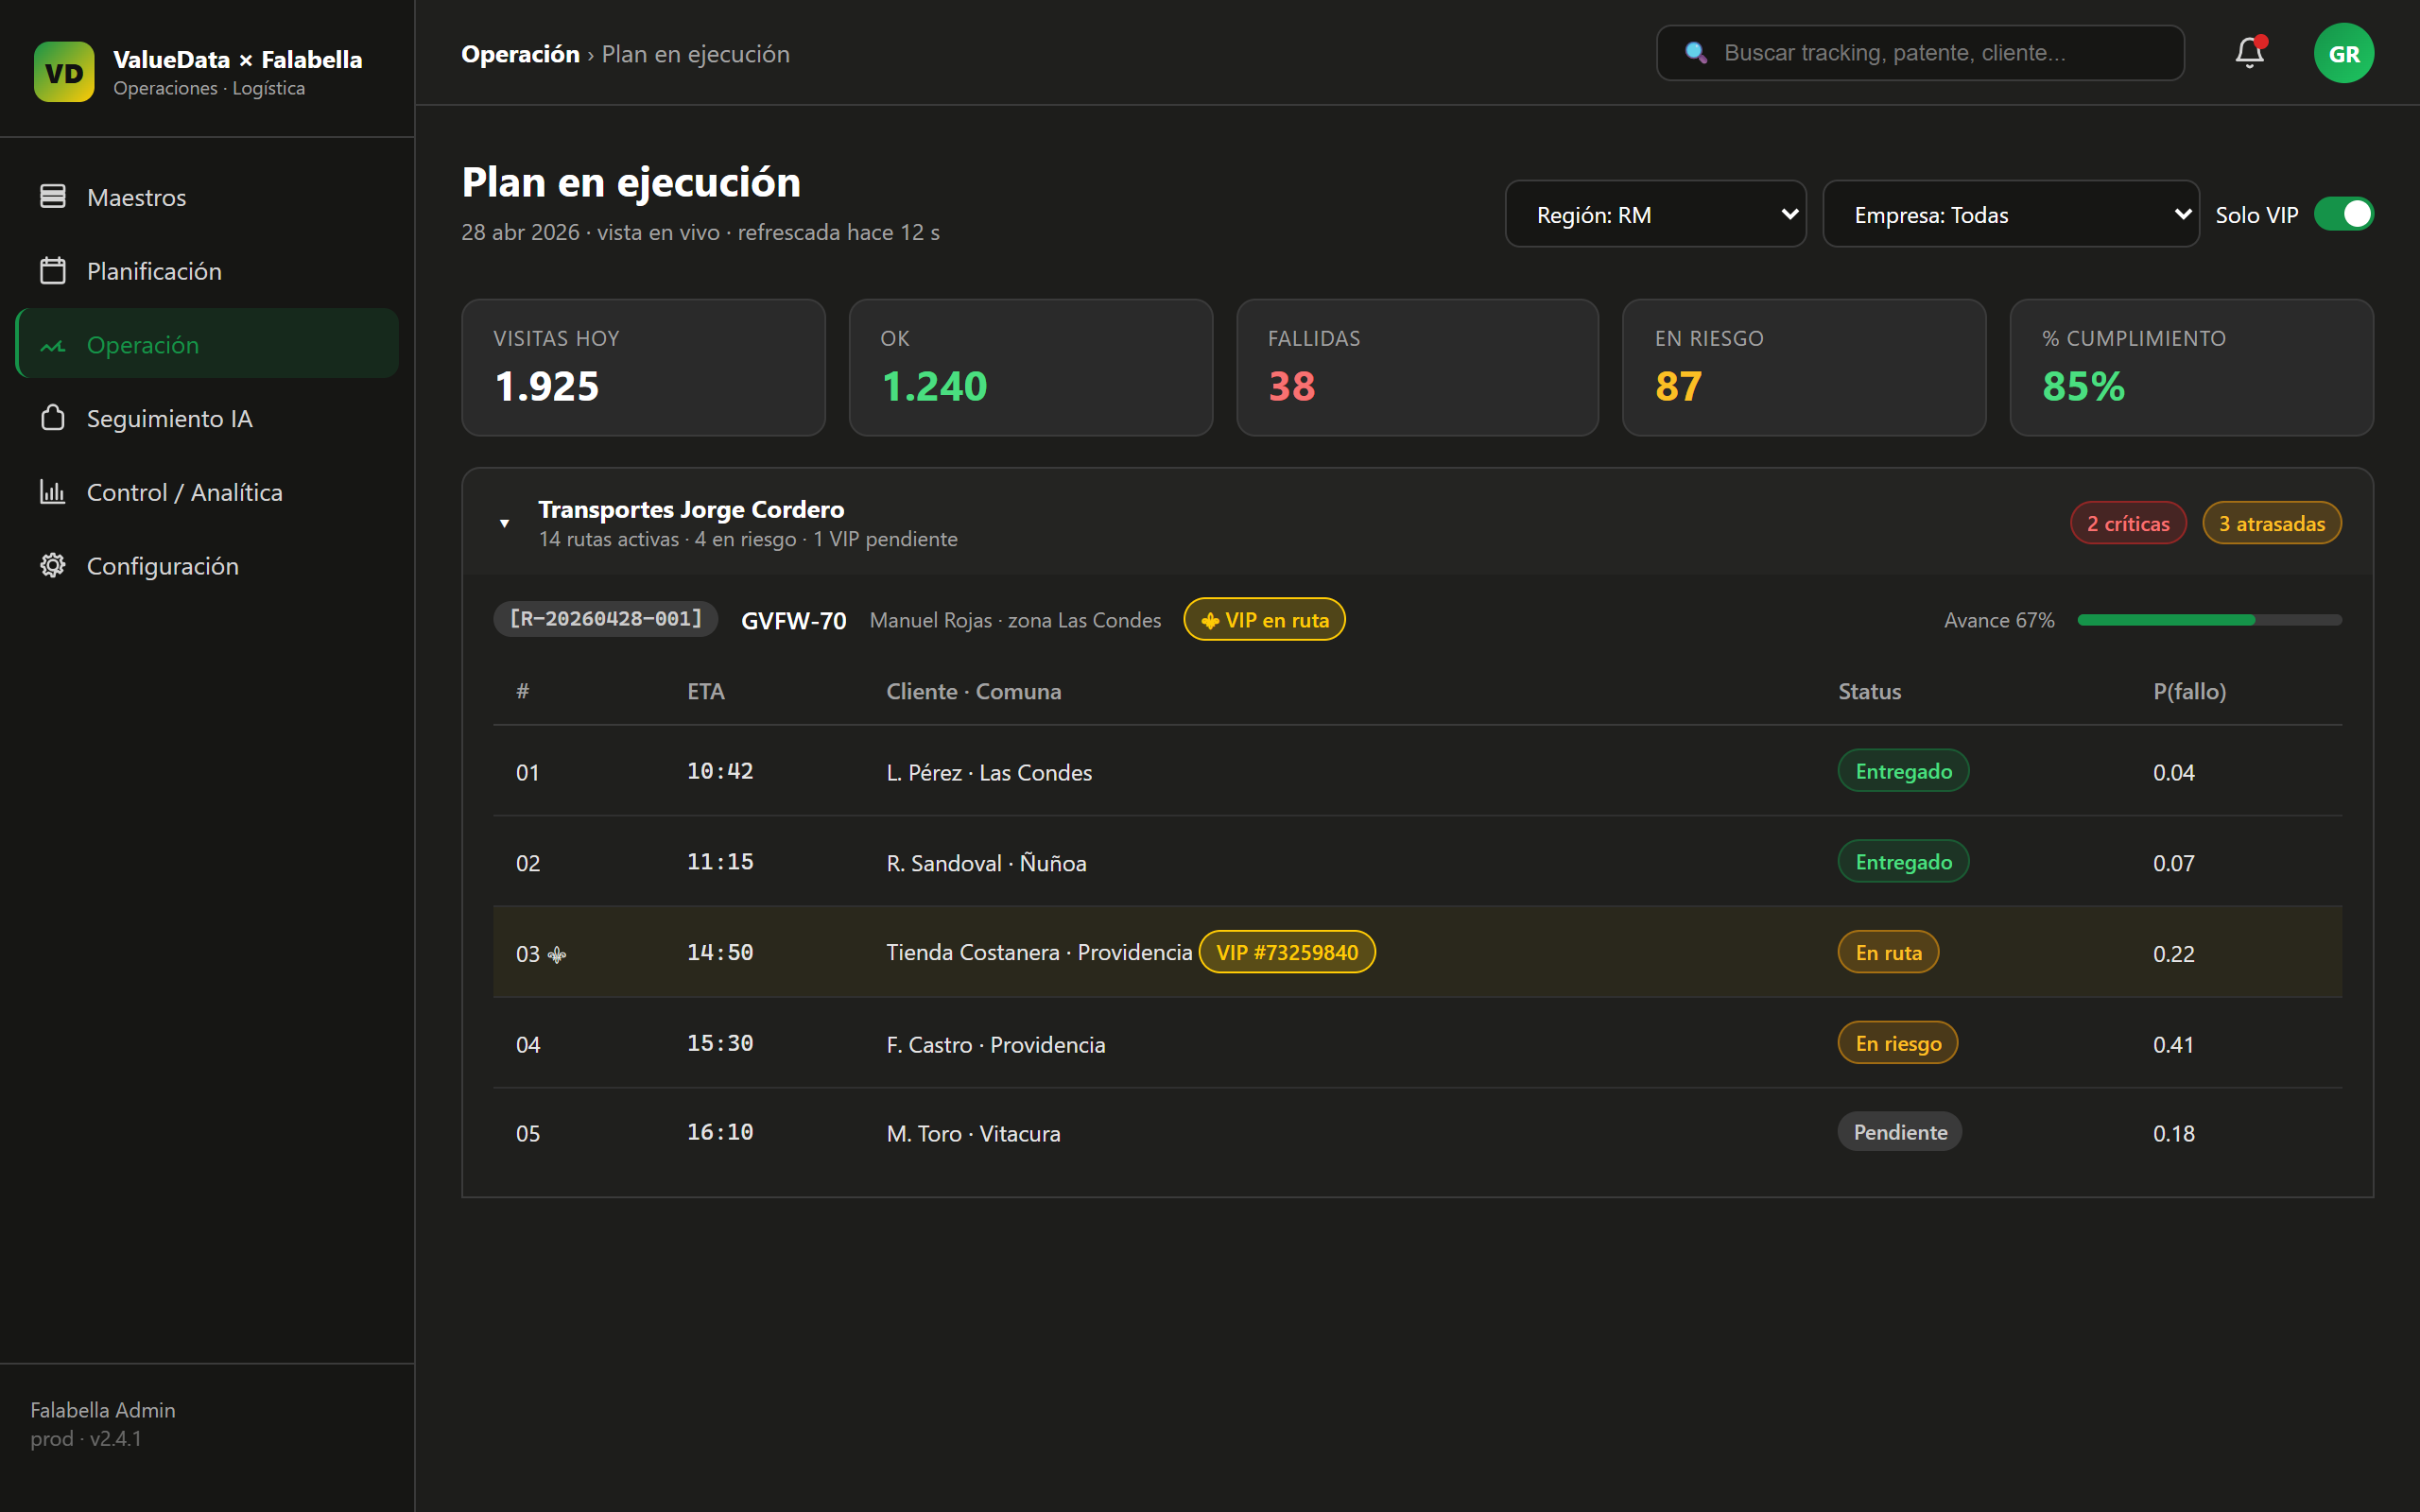
\includegraphics[width=0.95\textwidth]{07_plan_diario.png}
\caption{Plan en ejecucion: filtros globales arriba (region, empresa, toggle solo VIP), KPI strip con visitas / OK / fallidas / en riesgo / \% cumplimiento, y la jerarquia Empresa $\rightarrow$ Ruta $\rightarrow$ Visitas. La fila VIP destacada lleva chip dorado con el folio.}
\end{figure}

Es la \textbf{pantalla mas usada del dia}. Muestra todo el plan en
tiempo real con jerarquia de tres niveles.

\subsubsection{Jerarquia Empresa $\rightarrow$ Ruta $\rightarrow$ Visitas}

\begin{enumerate}
  \item \textbf{Empresa:} fila contraible al tope. Muestra nombre,
        cantidad de rutas, visitas totales, completadas, fallidas, en
        riesgo. Click expande/colapsa.
  \item \textbf{Ruta:} dentro de cada empresa, una fila por
        ruta\_id (vehiculo + dia). Header con
        \texttt{ruta\_id} en monospace, vehiculo, driver, cantidad de
        visitas, ETA estimada del cierre.
  \item \textbf{Visita:} dentro de cada ruta, una fila por visita
        ordenada por orden de parada. Columnas: \#orden, cliente,
        direccion, ventana, ETA, slack, riesgo, estado, acciones.
\end{enumerate}

\subsubsection{Header de ruta con ruta\_id}

El \texttt{ruta\_id} (formato \texttt{R-2026-04-28-V012}) se muestra
en la cabecera de cada ruta para que el operador pueda referenciar la
ruta en sistemas externos. Click en el header expande/colapsa el
detalle de visitas.

\subsubsection{ETA siempre visible}

Cada fila de visita muestra la ETA estimada (mejor estimador
disponible: SimpliRoute + corrimiento por incidentes manuales). El
color del semaforo de slack es:

\begin{itemize}
  \item \textbf{Verde:} ETA dentro de la ventana, holgura $> 20$ min.
  \item \textbf{Amarillo:} holgura entre 0 y 20 min. Riesgo medio.
  \item \textbf{Rojo:} ETA posterior a window\_end. Atraso confirmado.
\end{itemize}

\subsubsection{Folio VIP destacado}

Si la visita matchea con un VIP del dia, el folio se muestra con un
\textbf{badge dorado de corona} (icono CMR). Al pasar el mouse, el
tooltip muestra el tier, hora limite y minutos restantes hasta la
alerta.

\subsubsection{Reportar motivo (chofer)}

El chofer (o el manager en su nombre) puede reportar un motivo de
no-entrega cuando una visita no se va a completar. Flujo:

\begin{enumerate}
  \item Haz clic en el icono de \textbf{megafono} (o ``Reportar
        motivo'') en la fila de la visita.
  \item Se abre un dialogo con dos campos:
    \begin{itemize}
      \item \textbf{Motivo:} dropdown con los 13 motivos del catalogo.
      \item \textbf{Comentario:} texto libre, hasta 2000 caracteres.
            Sugerencia: describir lo que paso en el lugar.
    \end{itemize}
  \item Haz clic en \textbf{Guardar}.
  \item El backend persiste el comentario y \emph{automaticamente}:
    \begin{itemize}
      \item Si el motivo es alertable, emite el evento
            \texttt{comment\_alert} y dispara WhatsApp a los
            destinatarios filtrados.
      \item Llama al LLM para validar que el motivo elegido coincide
            con el comentario. Si no coincide, crea una correccion
            sugerida (ver Seccion 8.3).
    \end{itemize}
  \item En la UI aparece un toast verde: ``Motivo reportado''. La fila
        muestra una insignia con el motivo.
\end{enumerate}

\warnbox{Una vez reportado, el comentario \emph{no} se puede borrar
desde la UI. Si la IA detecta error, el flujo correcto es esperar la
correccion en \emph{Seguimiento IA $\rightarrow$ Correcciones}, donde
el admin acepta o rechaza la sugerencia.}

\subsection{Watchlist}

\begin{figure}[H]
\centering
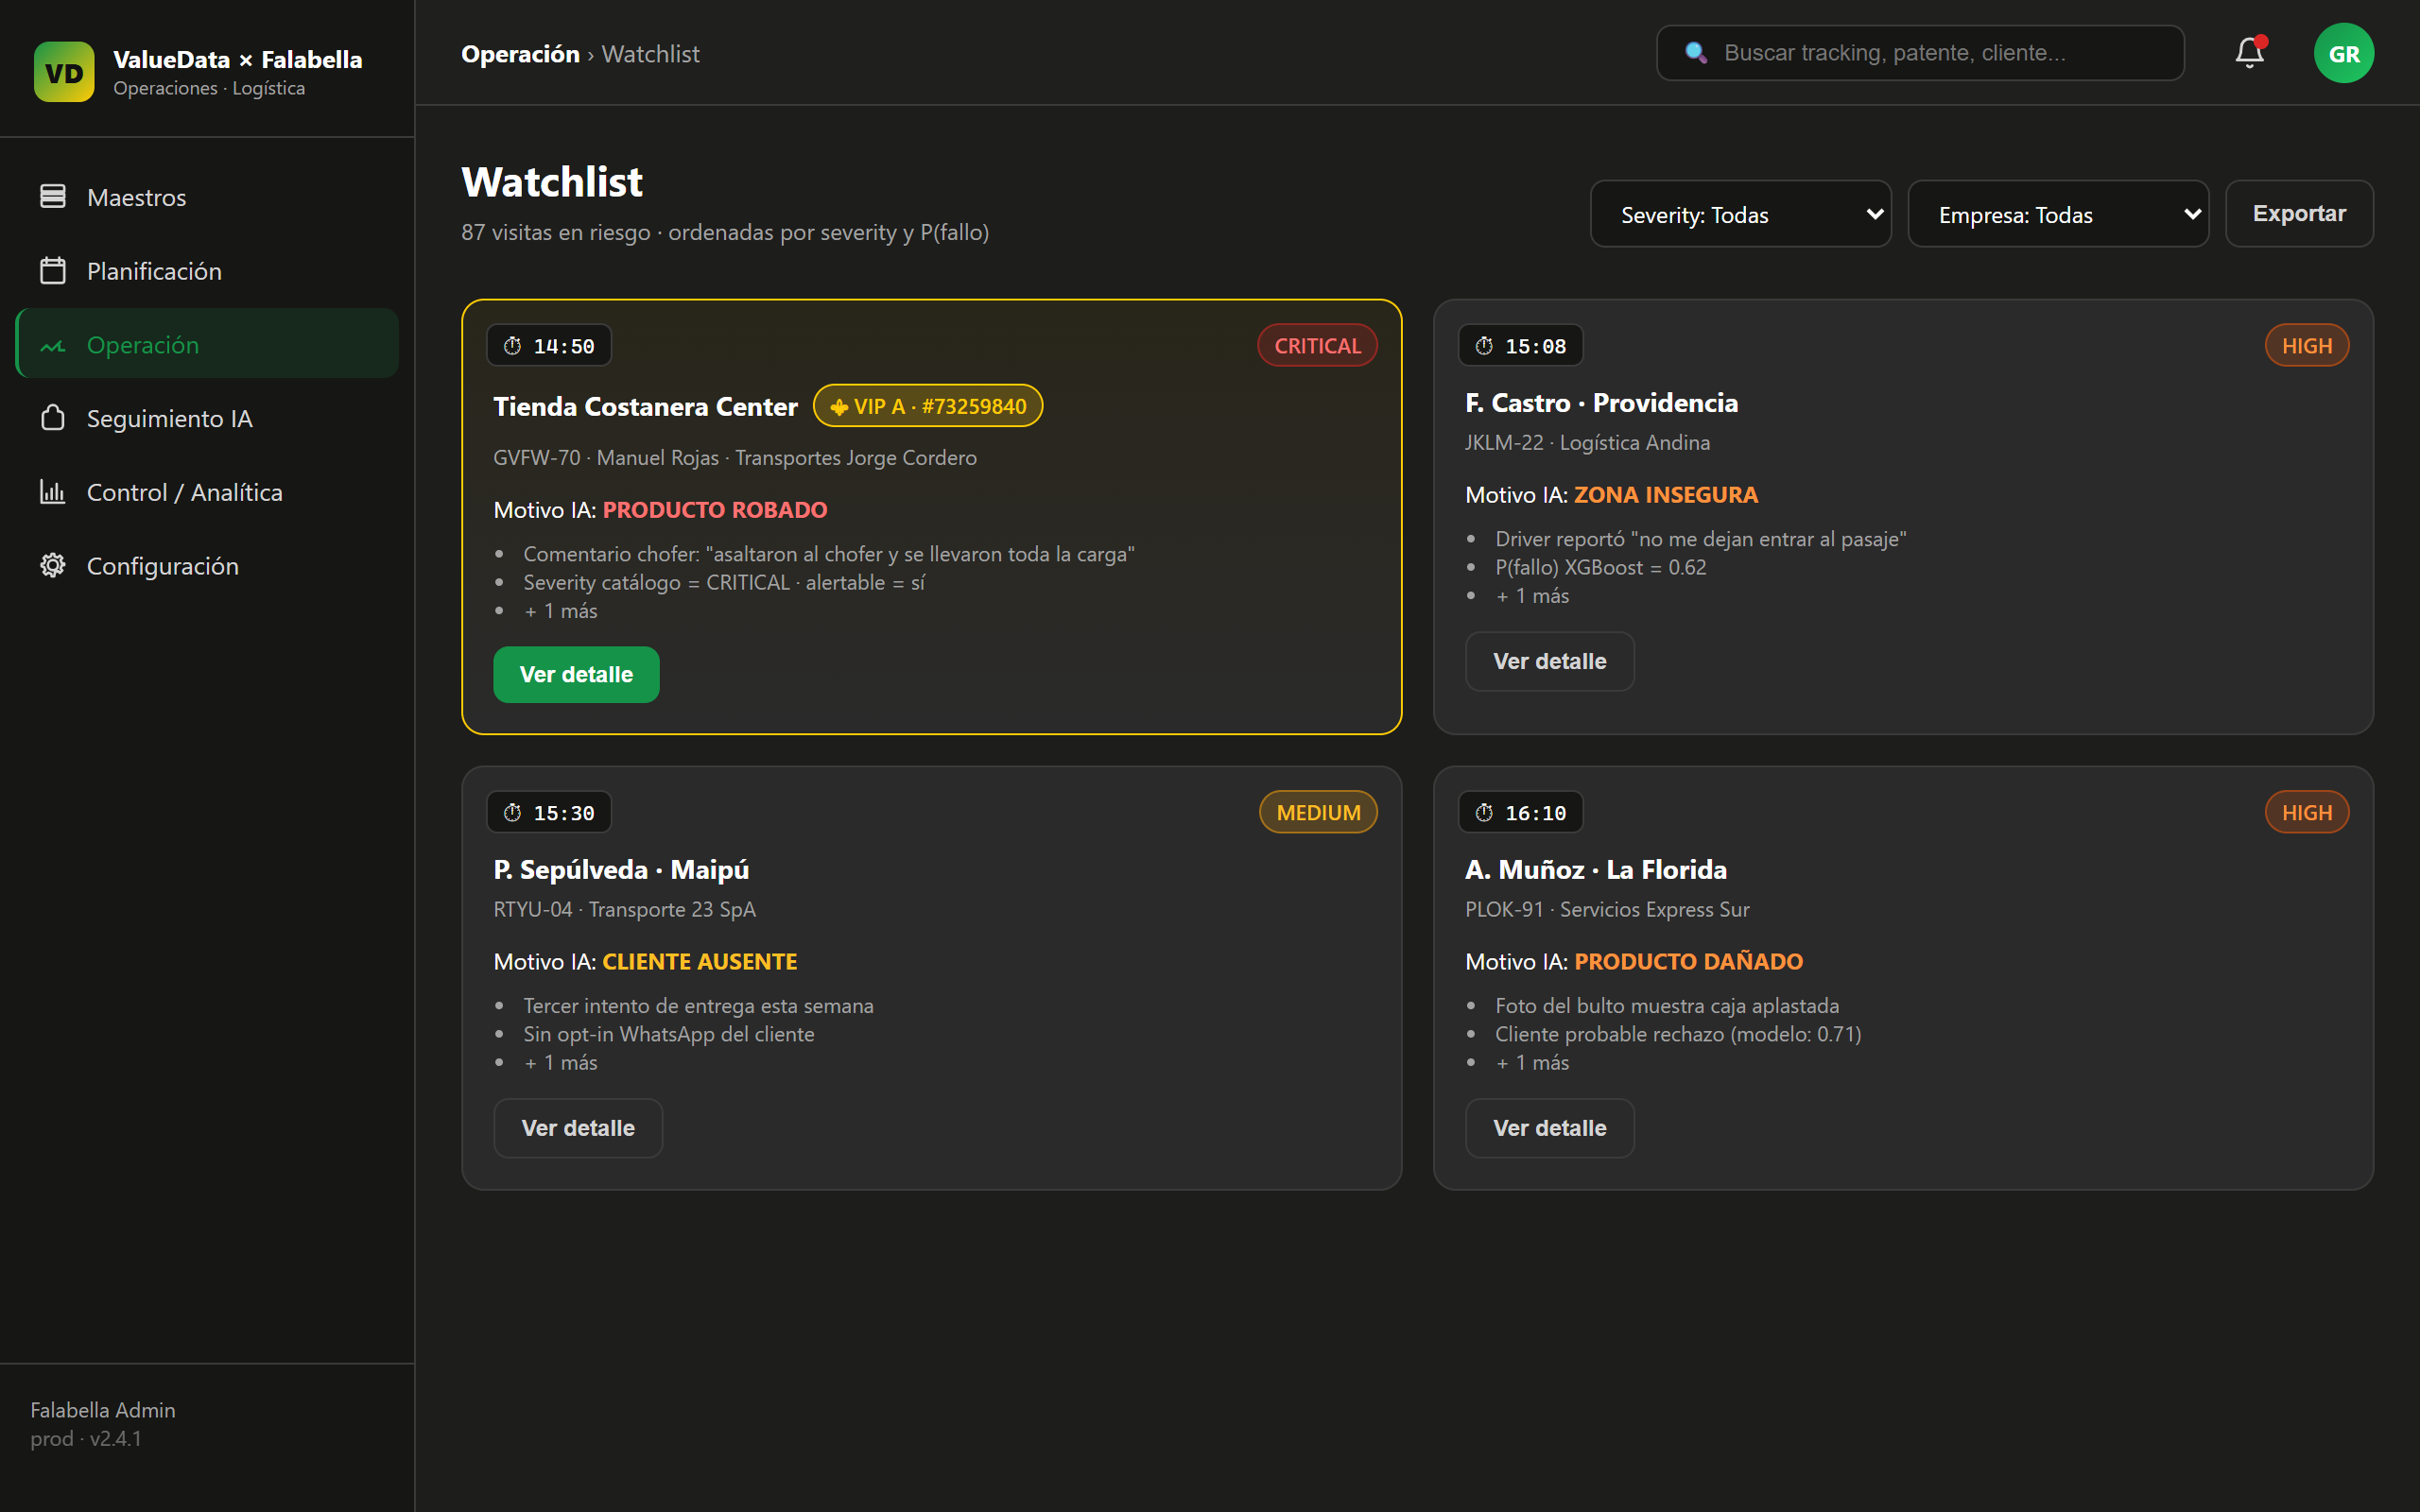
\includegraphics[width=0.95\textwidth]{08_watchlist.png}
\caption{Watchlist: cards con chip de severity (CRITICAL, HIGH, MEDIUM) en la esquina superior derecha, ETA en la izquierda, motivo IA, dos razones principales y boton Ver detalle. Las cards VIP llevan borde y chip dorado.}
\end{figure}

Lista priorizada de las visitas en riesgo. Refresca cada 5 segundos.

Encabezado con tarjetas-resumen clickeables: Total, Critico, Alto,
Medio, VIP en riesgo, Sin notificar. Click en una tarjeta filtra la
tabla por esa severidad.

Filtros adicionales: buscador por cliente / vehiculo / driver,
empresa (admin), notificadas / no notificadas, region, solo VIP.

Cada fila muestra: severidad, cliente (con badge VIP si aplica),
empresa, vehiculo, driver, ventana, ETA, slack, p(fallo),
last\_known\_alert (si la visita ya disparo alerta WhatsApp). Boton
\textbf{Notificar manualmente} permite emitir un broadcast adhoc al
contacto de la empresa.

\subsection{Mapa}

\begin{figure}[H]
\centering
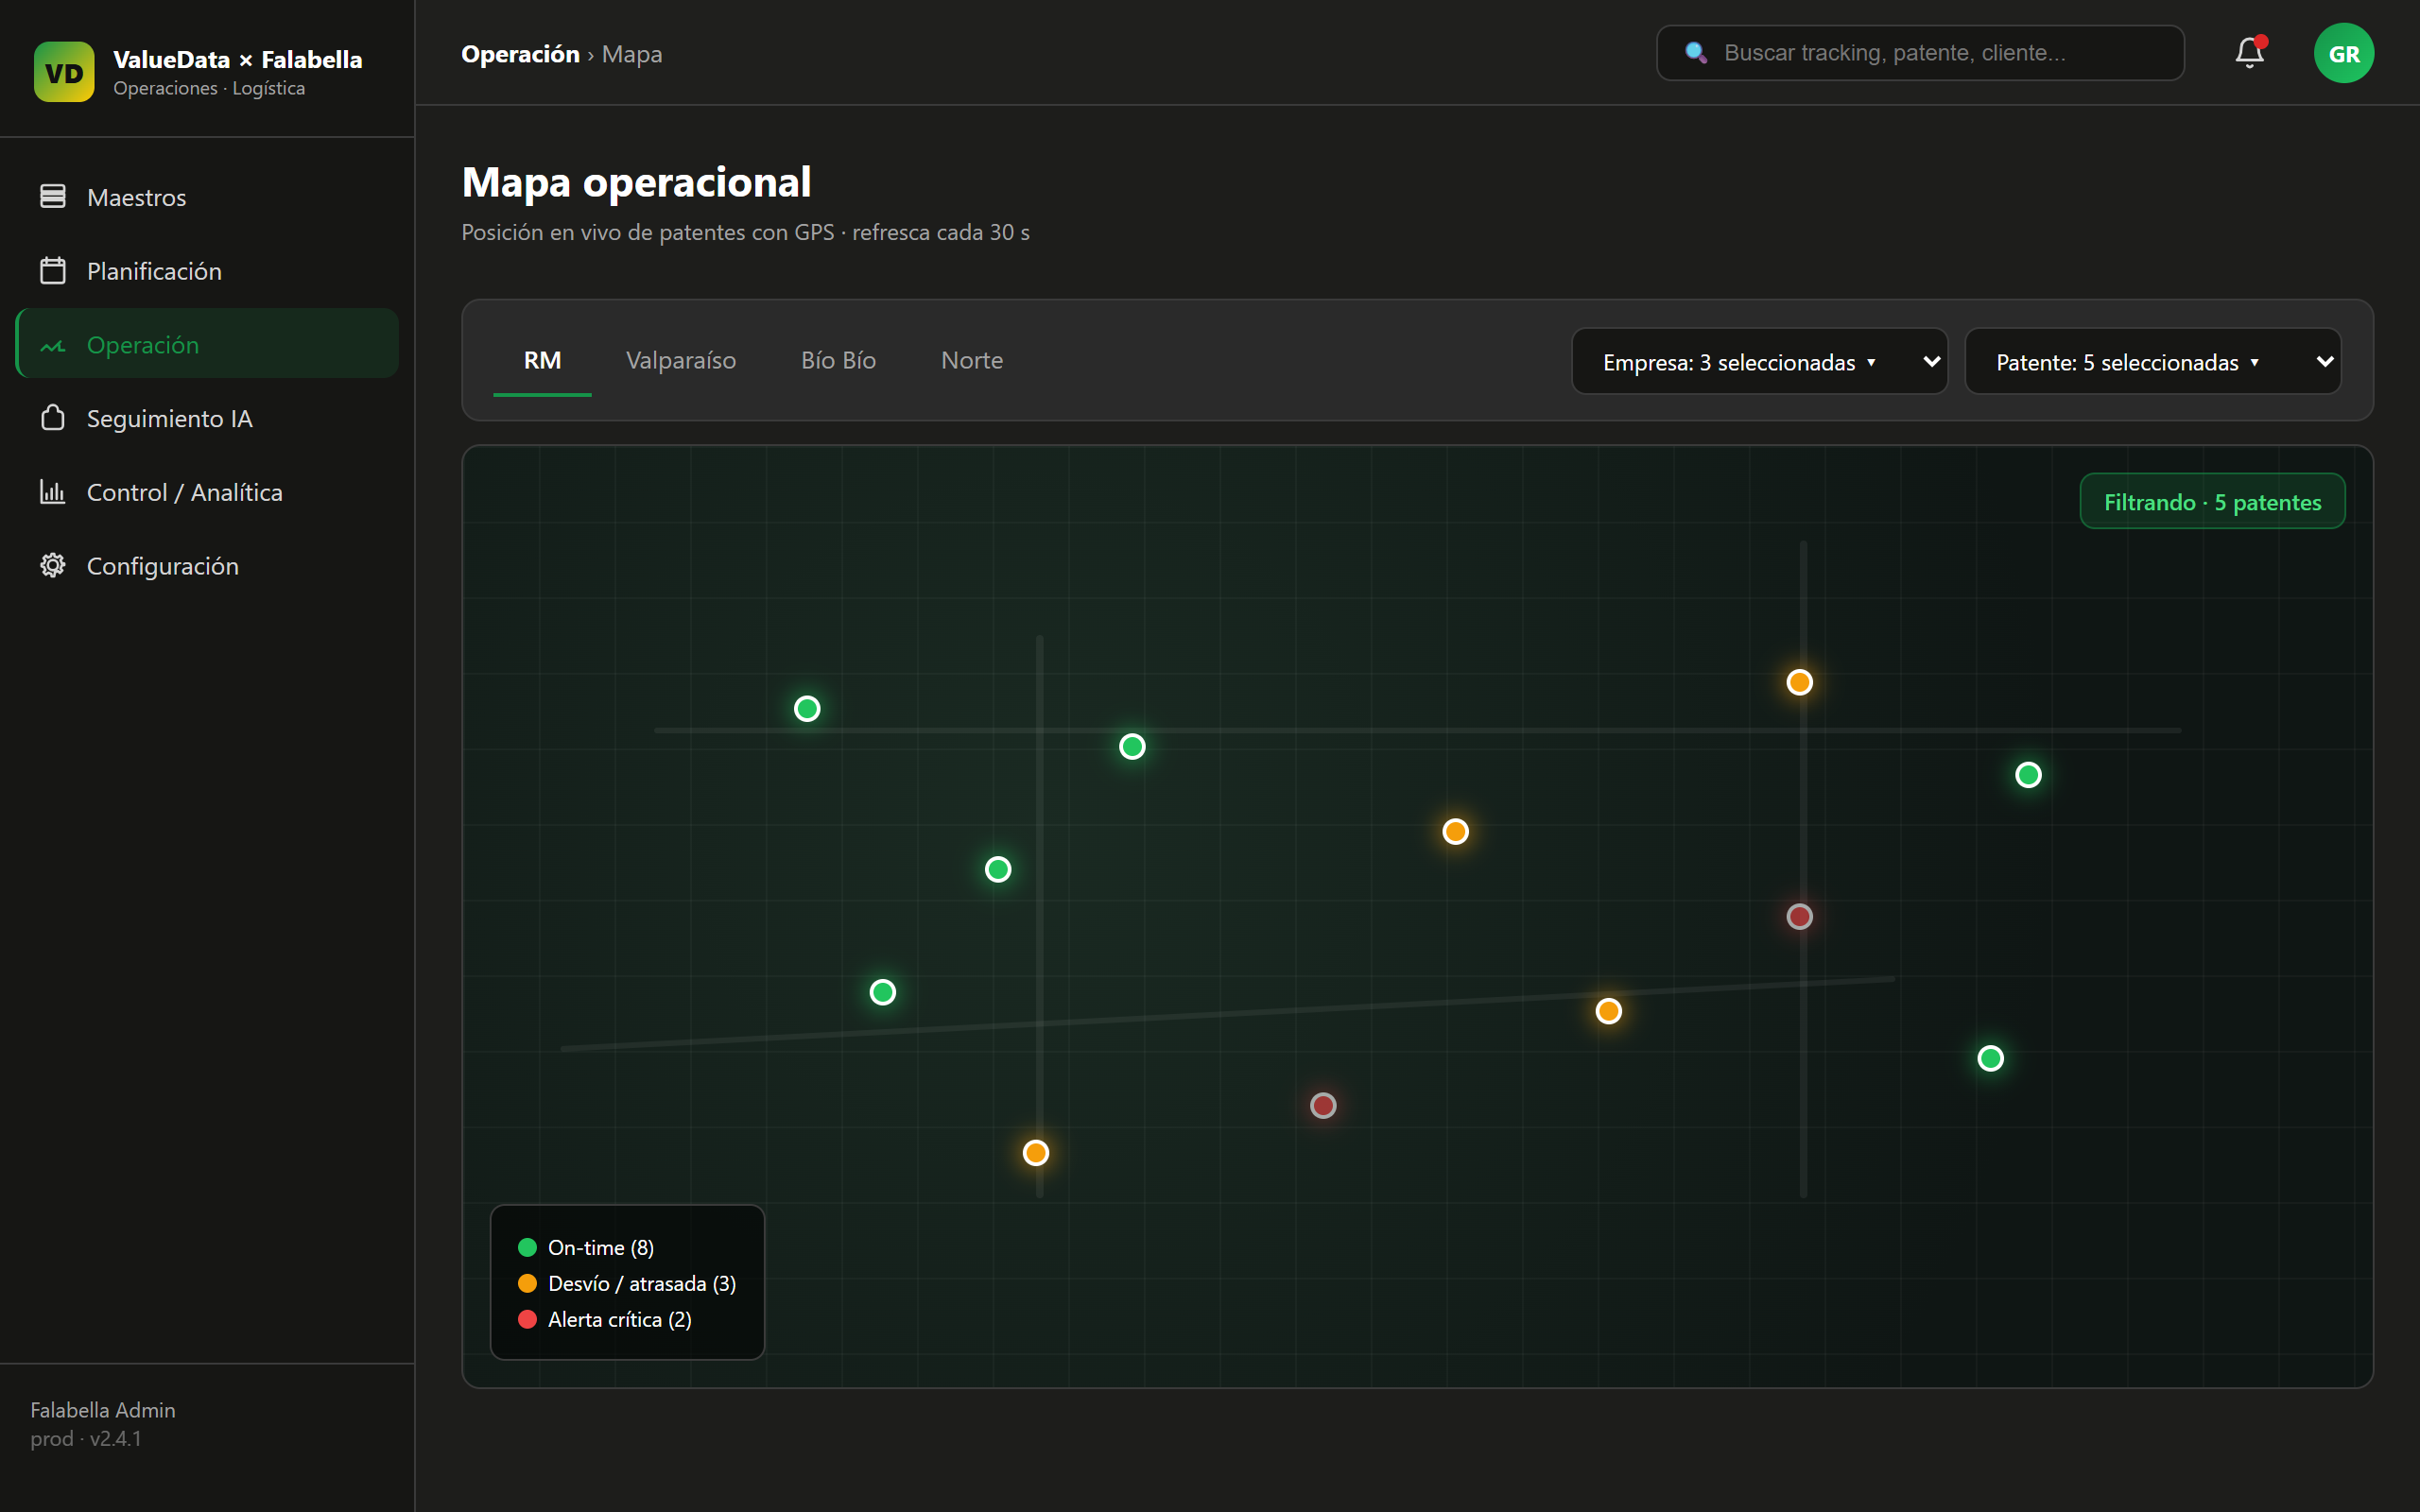
\includegraphics[width=0.95\textwidth]{09_mapa.png}
\caption{Mapa operacional: tabs por region y filtros multi-select de empresa y patente. Los puntos representan visitas (verde = on-time, ambar = desvio, rojo = alerta critica). El badge superior derecho indica los filtros activos.}
\end{figure}

Muestra todas las visitas como puntos en el mapa de Chile. Color
del punto = p(fallo) (verde a rojo segun magnitud). Borde violeta =
alerta ValueData activa. Hover muestra tooltip con tracking, cliente,
ETA y vehiculo.

Sirve para visualizar geograficamente donde se concentran los riesgos
del dia, y para detectar zonas problematicas (varias visitas rojas
agrupadas indican un sector con cobertura debil).

\subsection{Alertas en vivo}

Stream de eventos del dia, ordenado por hora descendente. Refresca
cada 4 segundos. Cada fila muestra:

\begin{itemize}
  \item Tipo de evento: motivo alertable, deadline VIP, correccion IA,
        falla, entrega, incidente, etc.
  \item Hora del evento (sim\_ts) en HH:MM.
  \item Detalle relevante: cliente, vehiculo, motivo, comentario.
  \item \texttt{tracking\_id} en monospace para referencia.
\end{itemize}

% =============================================================================
\section{Modulo SEGUIMIENTO IA}
% =============================================================================

Aqui es donde la IA \emph{audita} los reportes de los choferes. Tres
sub-tabs.

\subsection{Comentarios recientes}

Muestra los ultimos 80 eventos relevantes para auditoria IA filtrados a
tres tipos: \texttt{comment\_alert} (motivo alertable),
\texttt{vip\_deadline\_warning} y
\texttt{motivo\_correction\_suggested}. Refresca cada 4 segundos.

Cada fila muestra el motivo con color por severidad, el cliente, el
vehiculo, la ventana, el tracking y la hora. Cuando hay correccion IA,
se muestra ``\texttt{motivo\_reportado} $\rightarrow$
\texttt{motivo\_sugerido}'' y el razonamiento del LLM en italica.

\subsection{Asistente IA (validar comentarios manualmente)}

\begin{figure}[H]
\centering
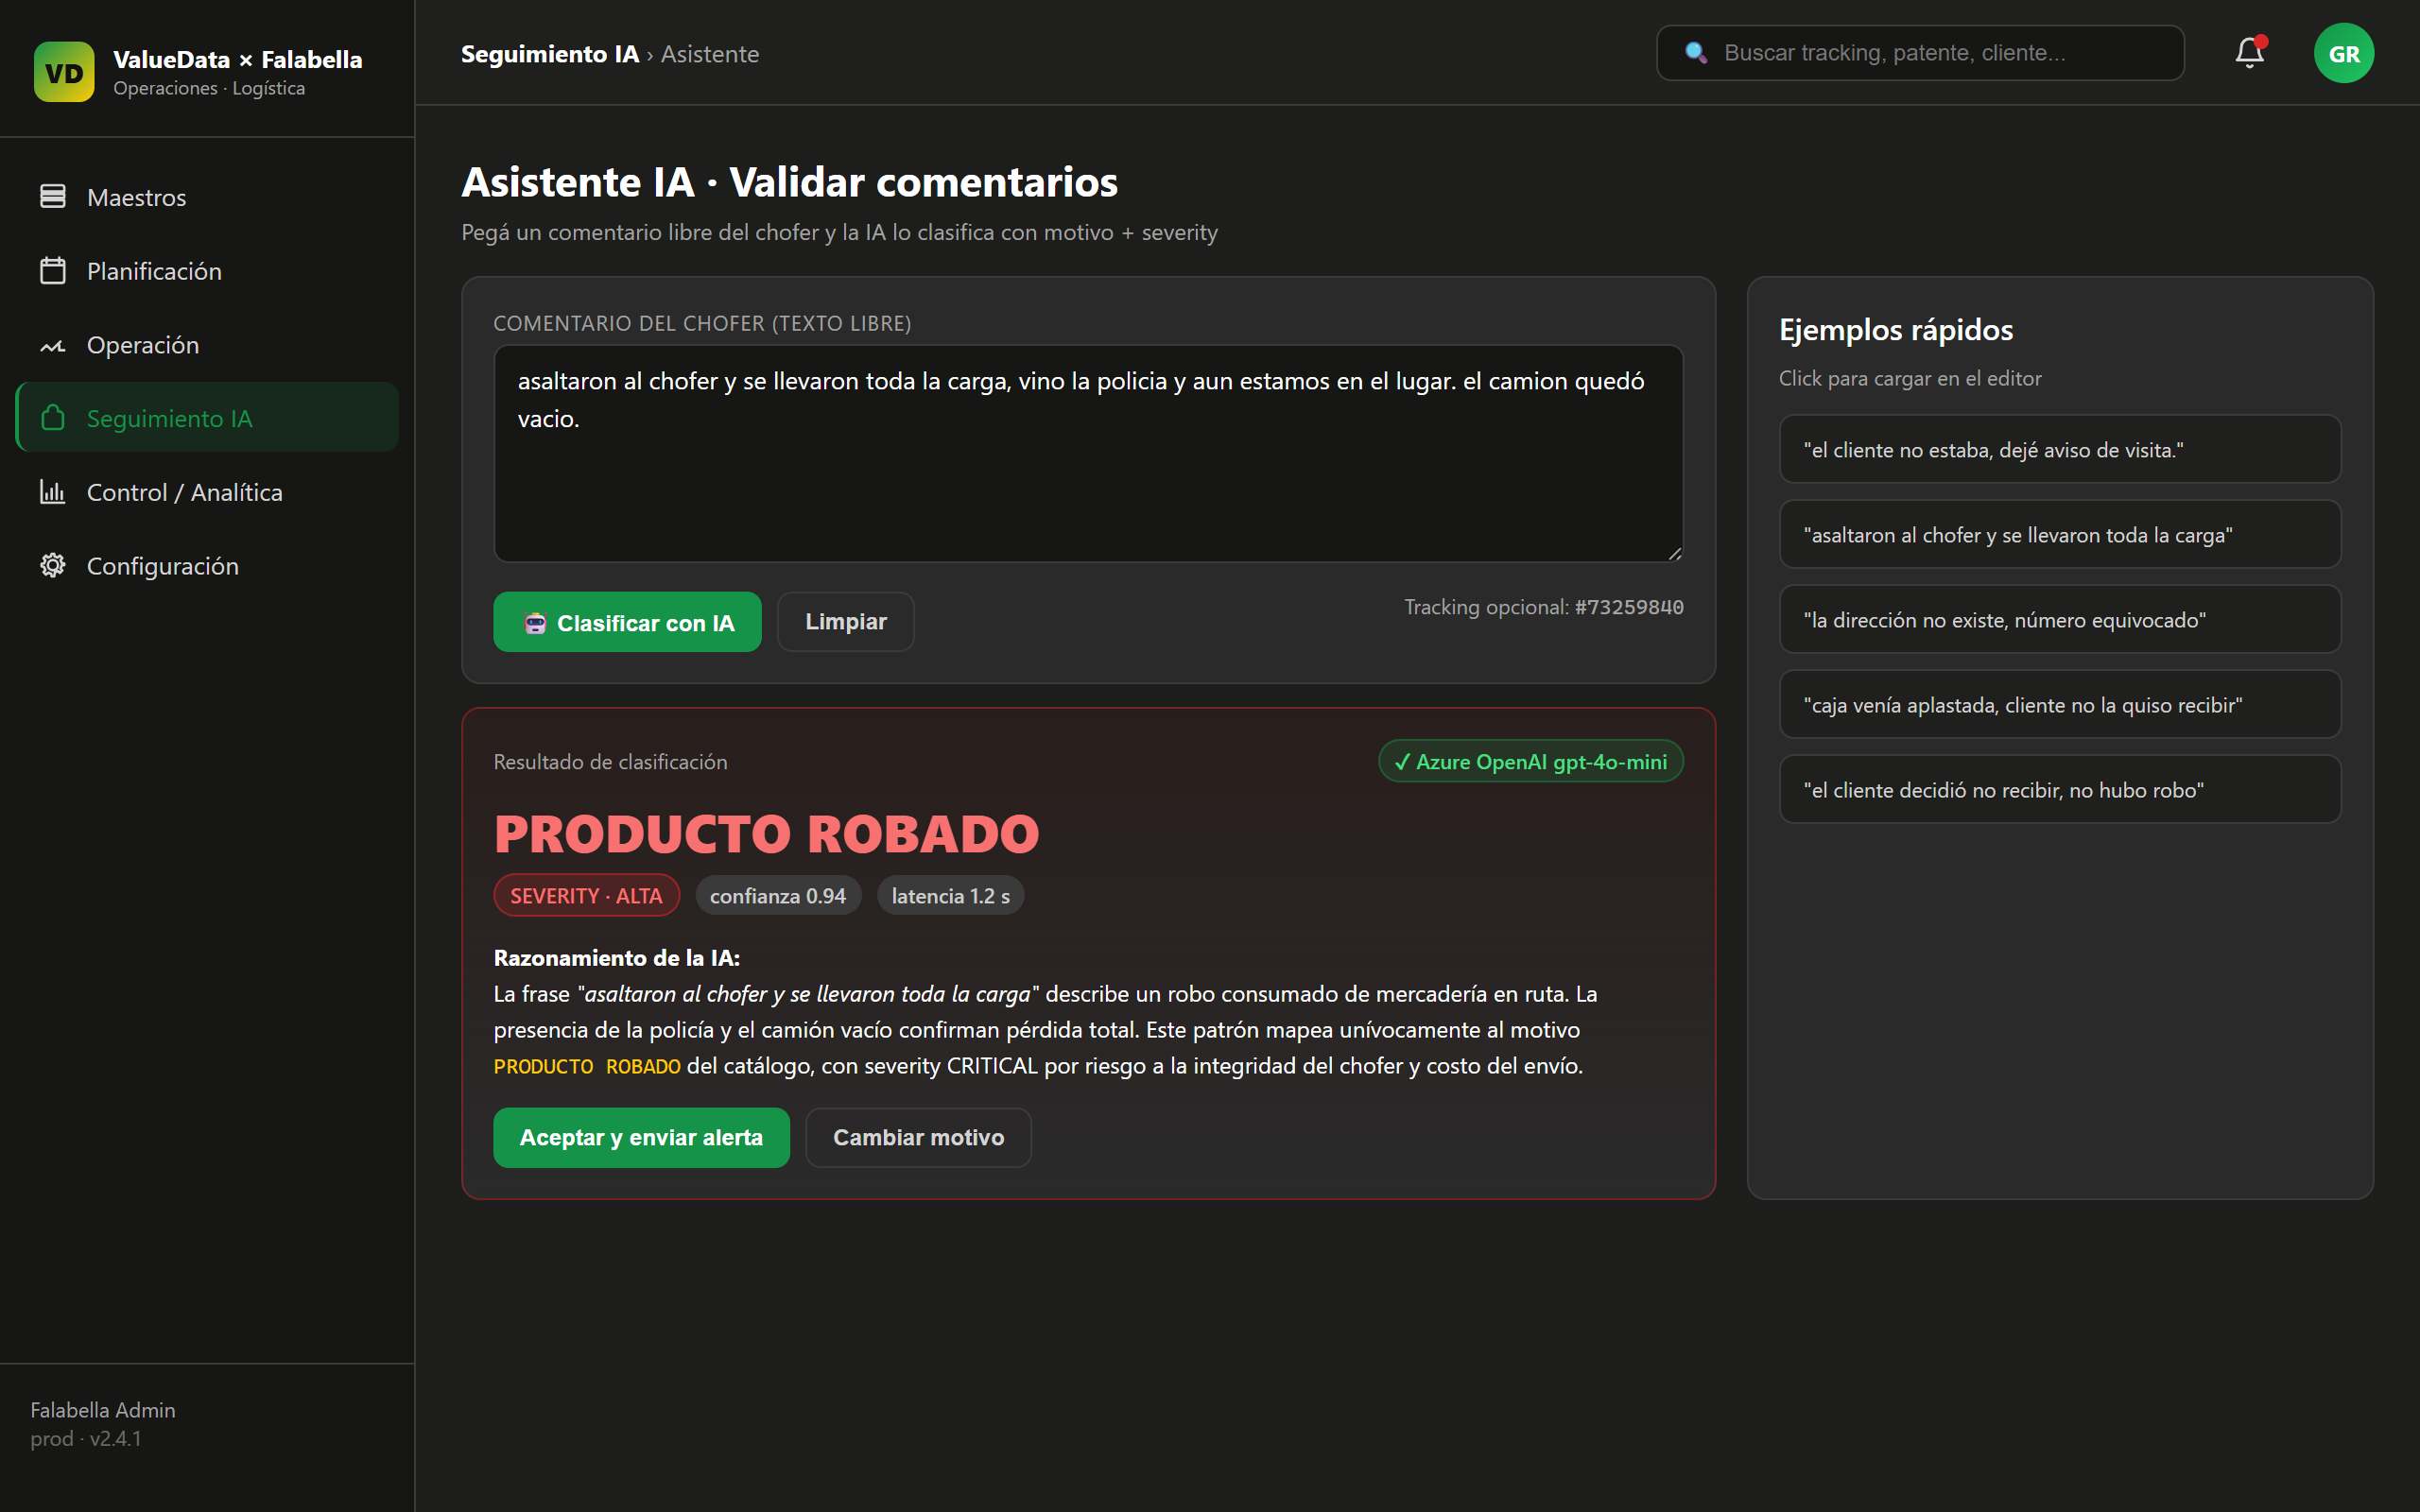
\includegraphics[width=0.95\textwidth]{10_asistente_ia.png}
\caption{Asistente IA: textarea con el comentario del chofer y boton Clasificar con IA. El resultado muestra el motivo en grande, la severity, el razonamiento del modelo y la badge Azure OpenAI gpt-4o-mini. A la derecha, ejemplos rapidos clickeables.}
\end{figure}

Pantalla donde un operador puede pedirle al LLM que clasifique un
comentario \emph{ad hoc} sin esperar a que ocurra el flujo automatico.

\begin{enumerate}
  \item Sidebar $\rightarrow$ Seguimiento IA $\rightarrow$
        Asistente IA.
  \item Pega el comentario del chofer en el campo de texto.
  \item Opcionalmente, indica el motivo que el chofer reporto.
  \item Haz clic en \textbf{Clasificar}.
  \item El LLM devuelve: motivo sugerido, confianza (alta / media /
        baja) y razonamiento.
\end{enumerate}

Util para entrenar a despachadores nuevos sobre como usar la IA.

\subsection{Correcciones de motivo}

\begin{figure}[H]
\centering
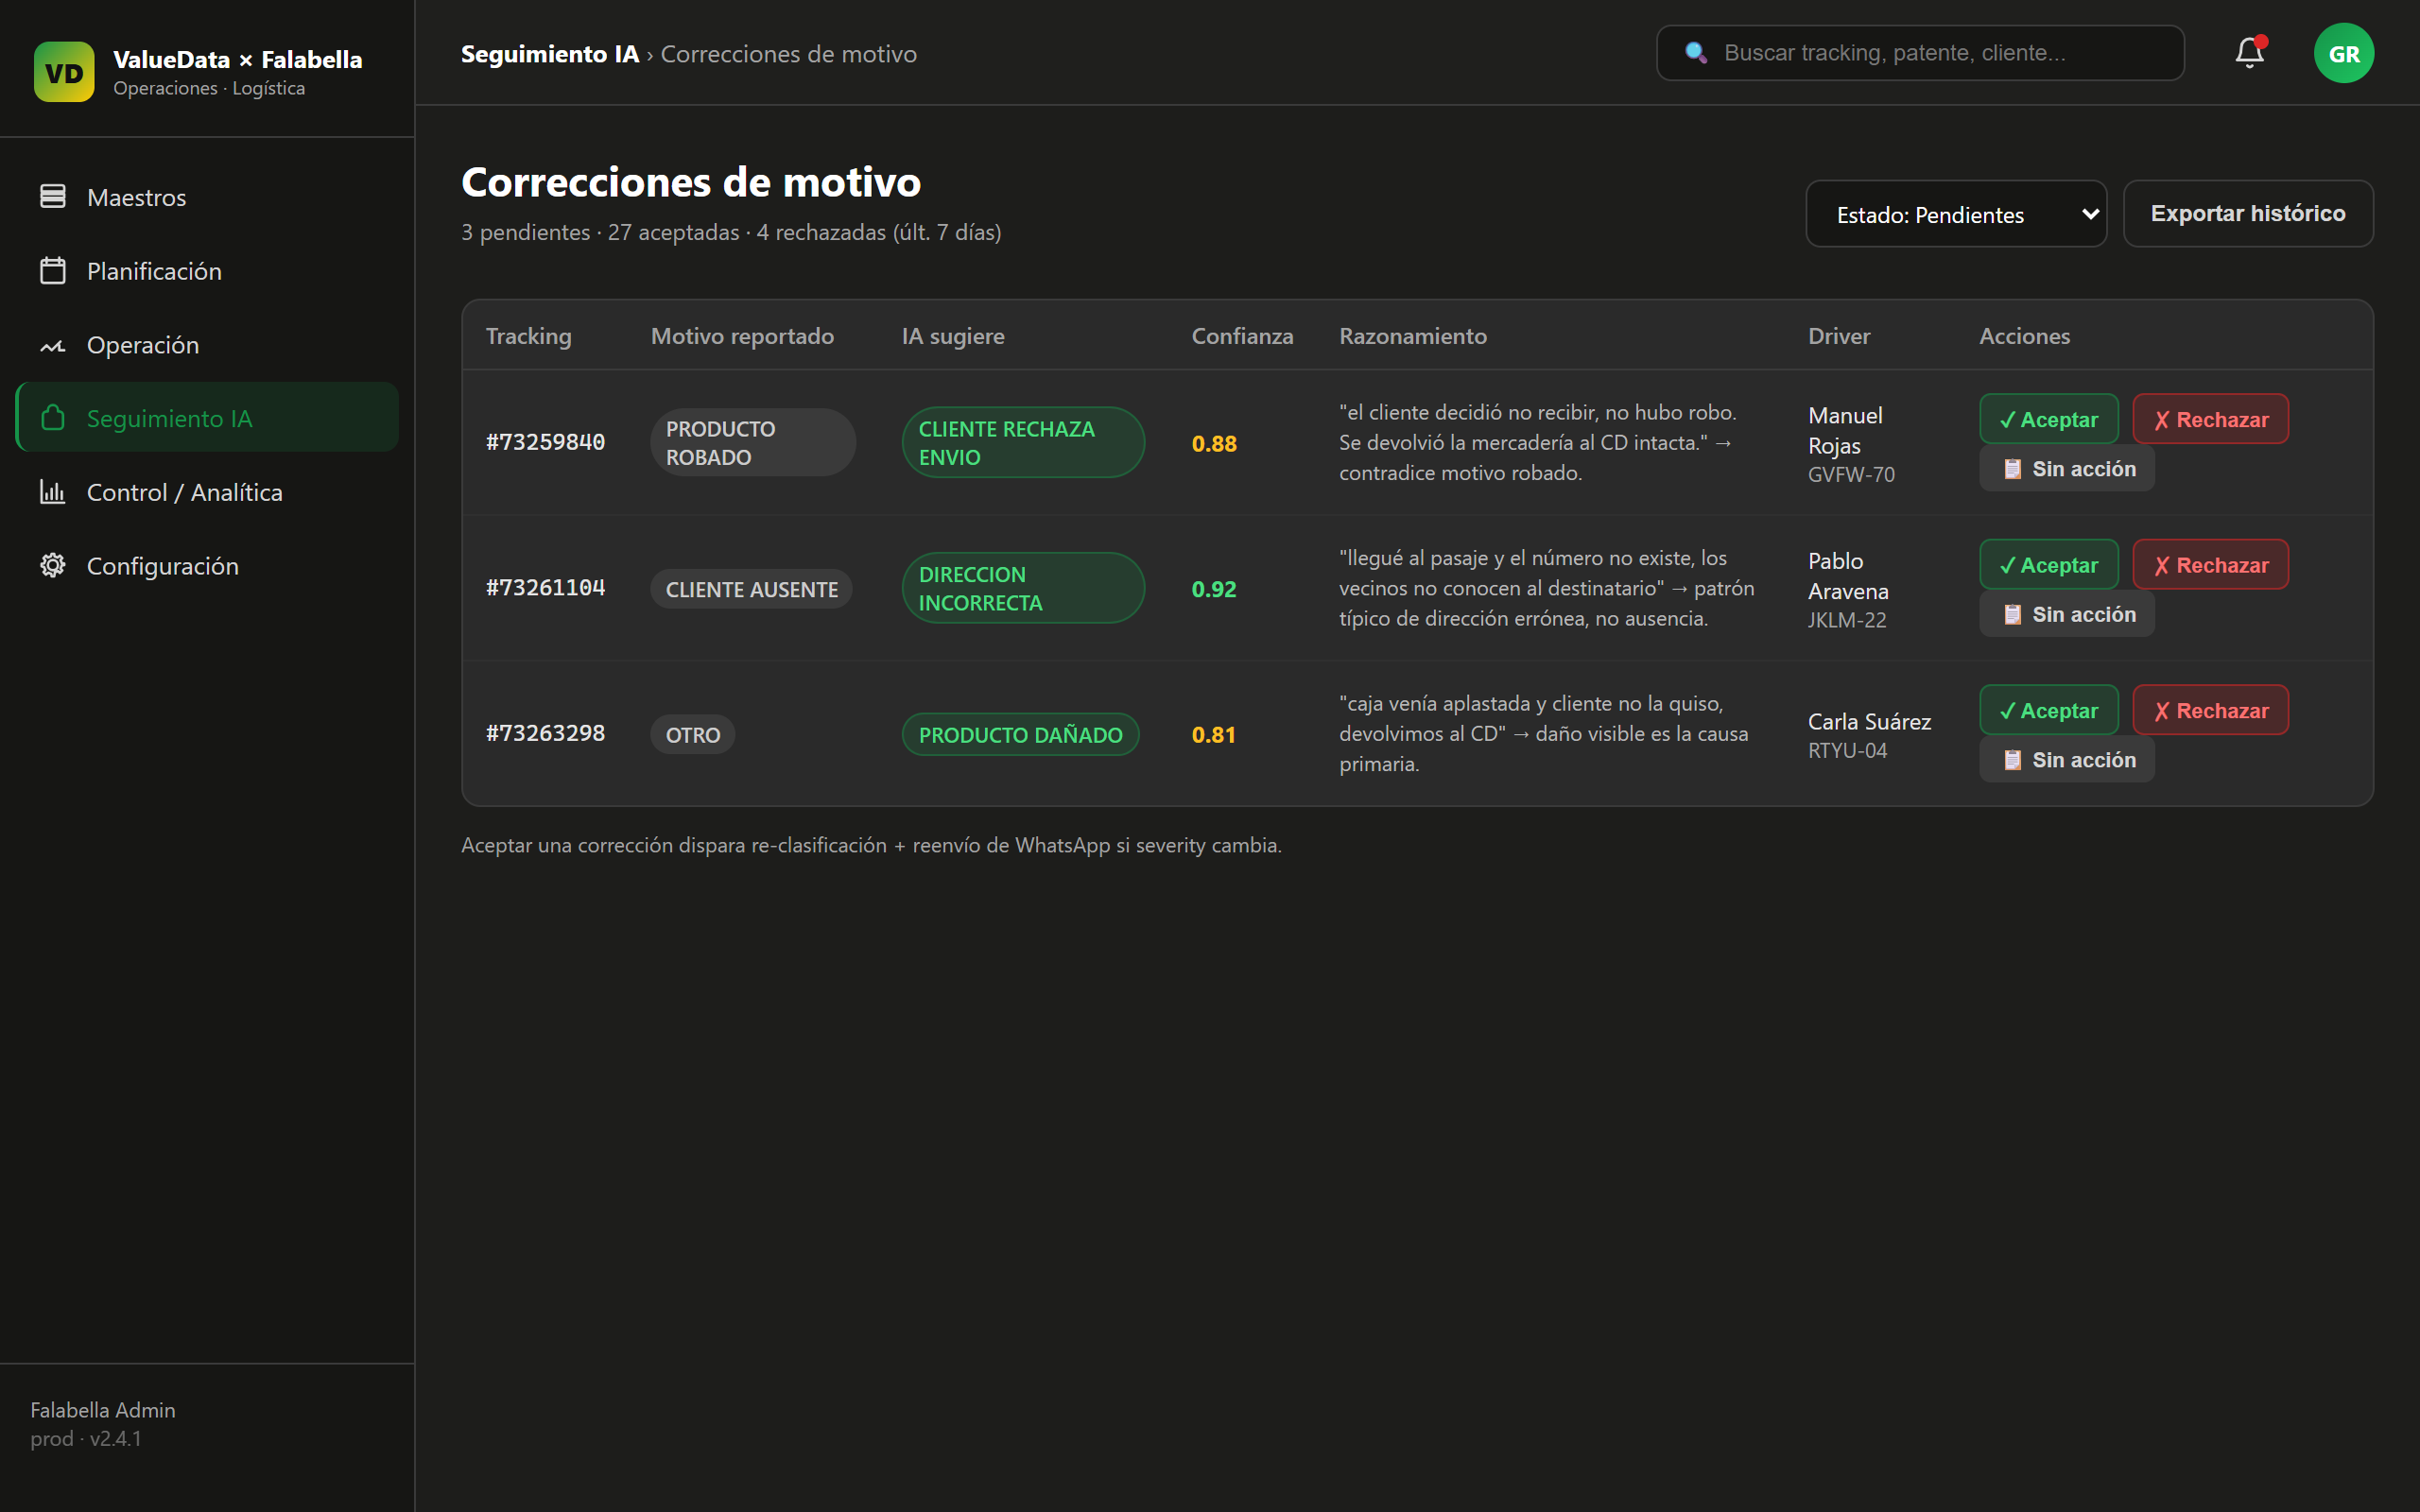
\includegraphics[width=0.95\textwidth]{11_correcciones_motivo.png}
\caption{Correcciones pendientes: tabla con tracking, motivo reportado, motivo sugerido por la IA, confianza, razonamiento, driver y acciones (Aceptar / Rechazar / Sin accion). Aceptar dispara re-clasificacion y reenvio de WhatsApp si la severity cambia.}
\end{figure}

Tabla de correcciones generadas automaticamente cuando la IA detecta
discrepancia entre el motivo reportado y lo que indica el comentario.
Refresca cada 8 segundos.

\subsubsection{Que es una correccion}

Cuando un chofer reporta un motivo, el backend invoca el LLM con el
comentario. Si el LLM sugiere un motivo distinto con confianza
\emph{alta} o \emph{media}, se crea una correccion en estado
\texttt{pending}. La correccion incluye:

\begin{itemize}
  \item \texttt{motivo\_reportado}: lo que puso el chofer.
  \item \texttt{motivo\_sugerido}: lo que el LLM cree que es.
  \item \texttt{confianza}: alta, media, baja.
  \item \texttt{razonamiento}: explicacion del LLM.
\end{itemize}

\subsubsection{Aceptar / Rechazar / Sin accion}

La pantalla tiene 5 pestanas de filtro: Pendientes, Aceptadas,
Rechazadas, Archivadas, Todas.

Por cada fila pending, hay tres botones:

\begin{itemize}
  \item \textbf{Aceptar} (check verde): aplica el motivo sugerido al
        comentario original (UPDATE en
        \texttt{fpoc\_visit\_comments}). Marca la correccion como
        \emph{accepted}. Si la nueva severidad escala, dispara
        re-dispatch.
  \item \textbf{Rechazar} (X roja): marca la correccion como
        \emph{rejected} sin tocar el comentario. El motivo original se
        mantiene.
  \item \textbf{Archivar} (icono gris): marca como \emph{no\_action}.
        Sirve para correcciones ambiguas que no quieres tomar pero
        tampoco rechazar.
  \item \textbf{Re-notificar driver} (campana): vuelve a enviar el
        WhatsApp de pedido de confirmacion al driver, util si el
        chofer no respondio.
\end{itemize}

\subsubsection{Re-dispatch automatico si severity escala}

Cuando aceptas una correccion, el backend compara la severidad efectiva
del motivo viejo vs el nuevo. Si:

\begin{enumerate}
  \item El motivo viejo NO era alertable y el nuevo SI lo es, OR
  \item Ambos son alertables pero el nuevo tiene severidad mayor
        (low $<$ medium $<$ high $<$ critical),
\end{enumerate}

\noindent entonces se considera \emph{escalado}. En ese caso el sistema
\textbf{vuelve a disparar la alerta WhatsApp} con prefijo
\emph{``\textbackslash{}emoji\{IA\} IA reclasifico:''} y notifica
nuevamente a los destinatarios. Esto evita perder casos donde el
chofer minimizo la criticidad real del evento.

\importantbox{Si la nueva severidad es menor o igual, no se hace
re-dispatch (no enviamos un WhatsApp ``oye era menos grave''). El
comentario simplemente queda corregido en la base de datos.}

% =============================================================================
\section{Modulo CONTROL / ANALITICA}
% =============================================================================

Cuatro sub-tabs: KPIs, Driver scorecard, Notificaciones log,
Modelo XGB.

\subsection{KPIs historicos}

\begin{figure}[H]
\centering
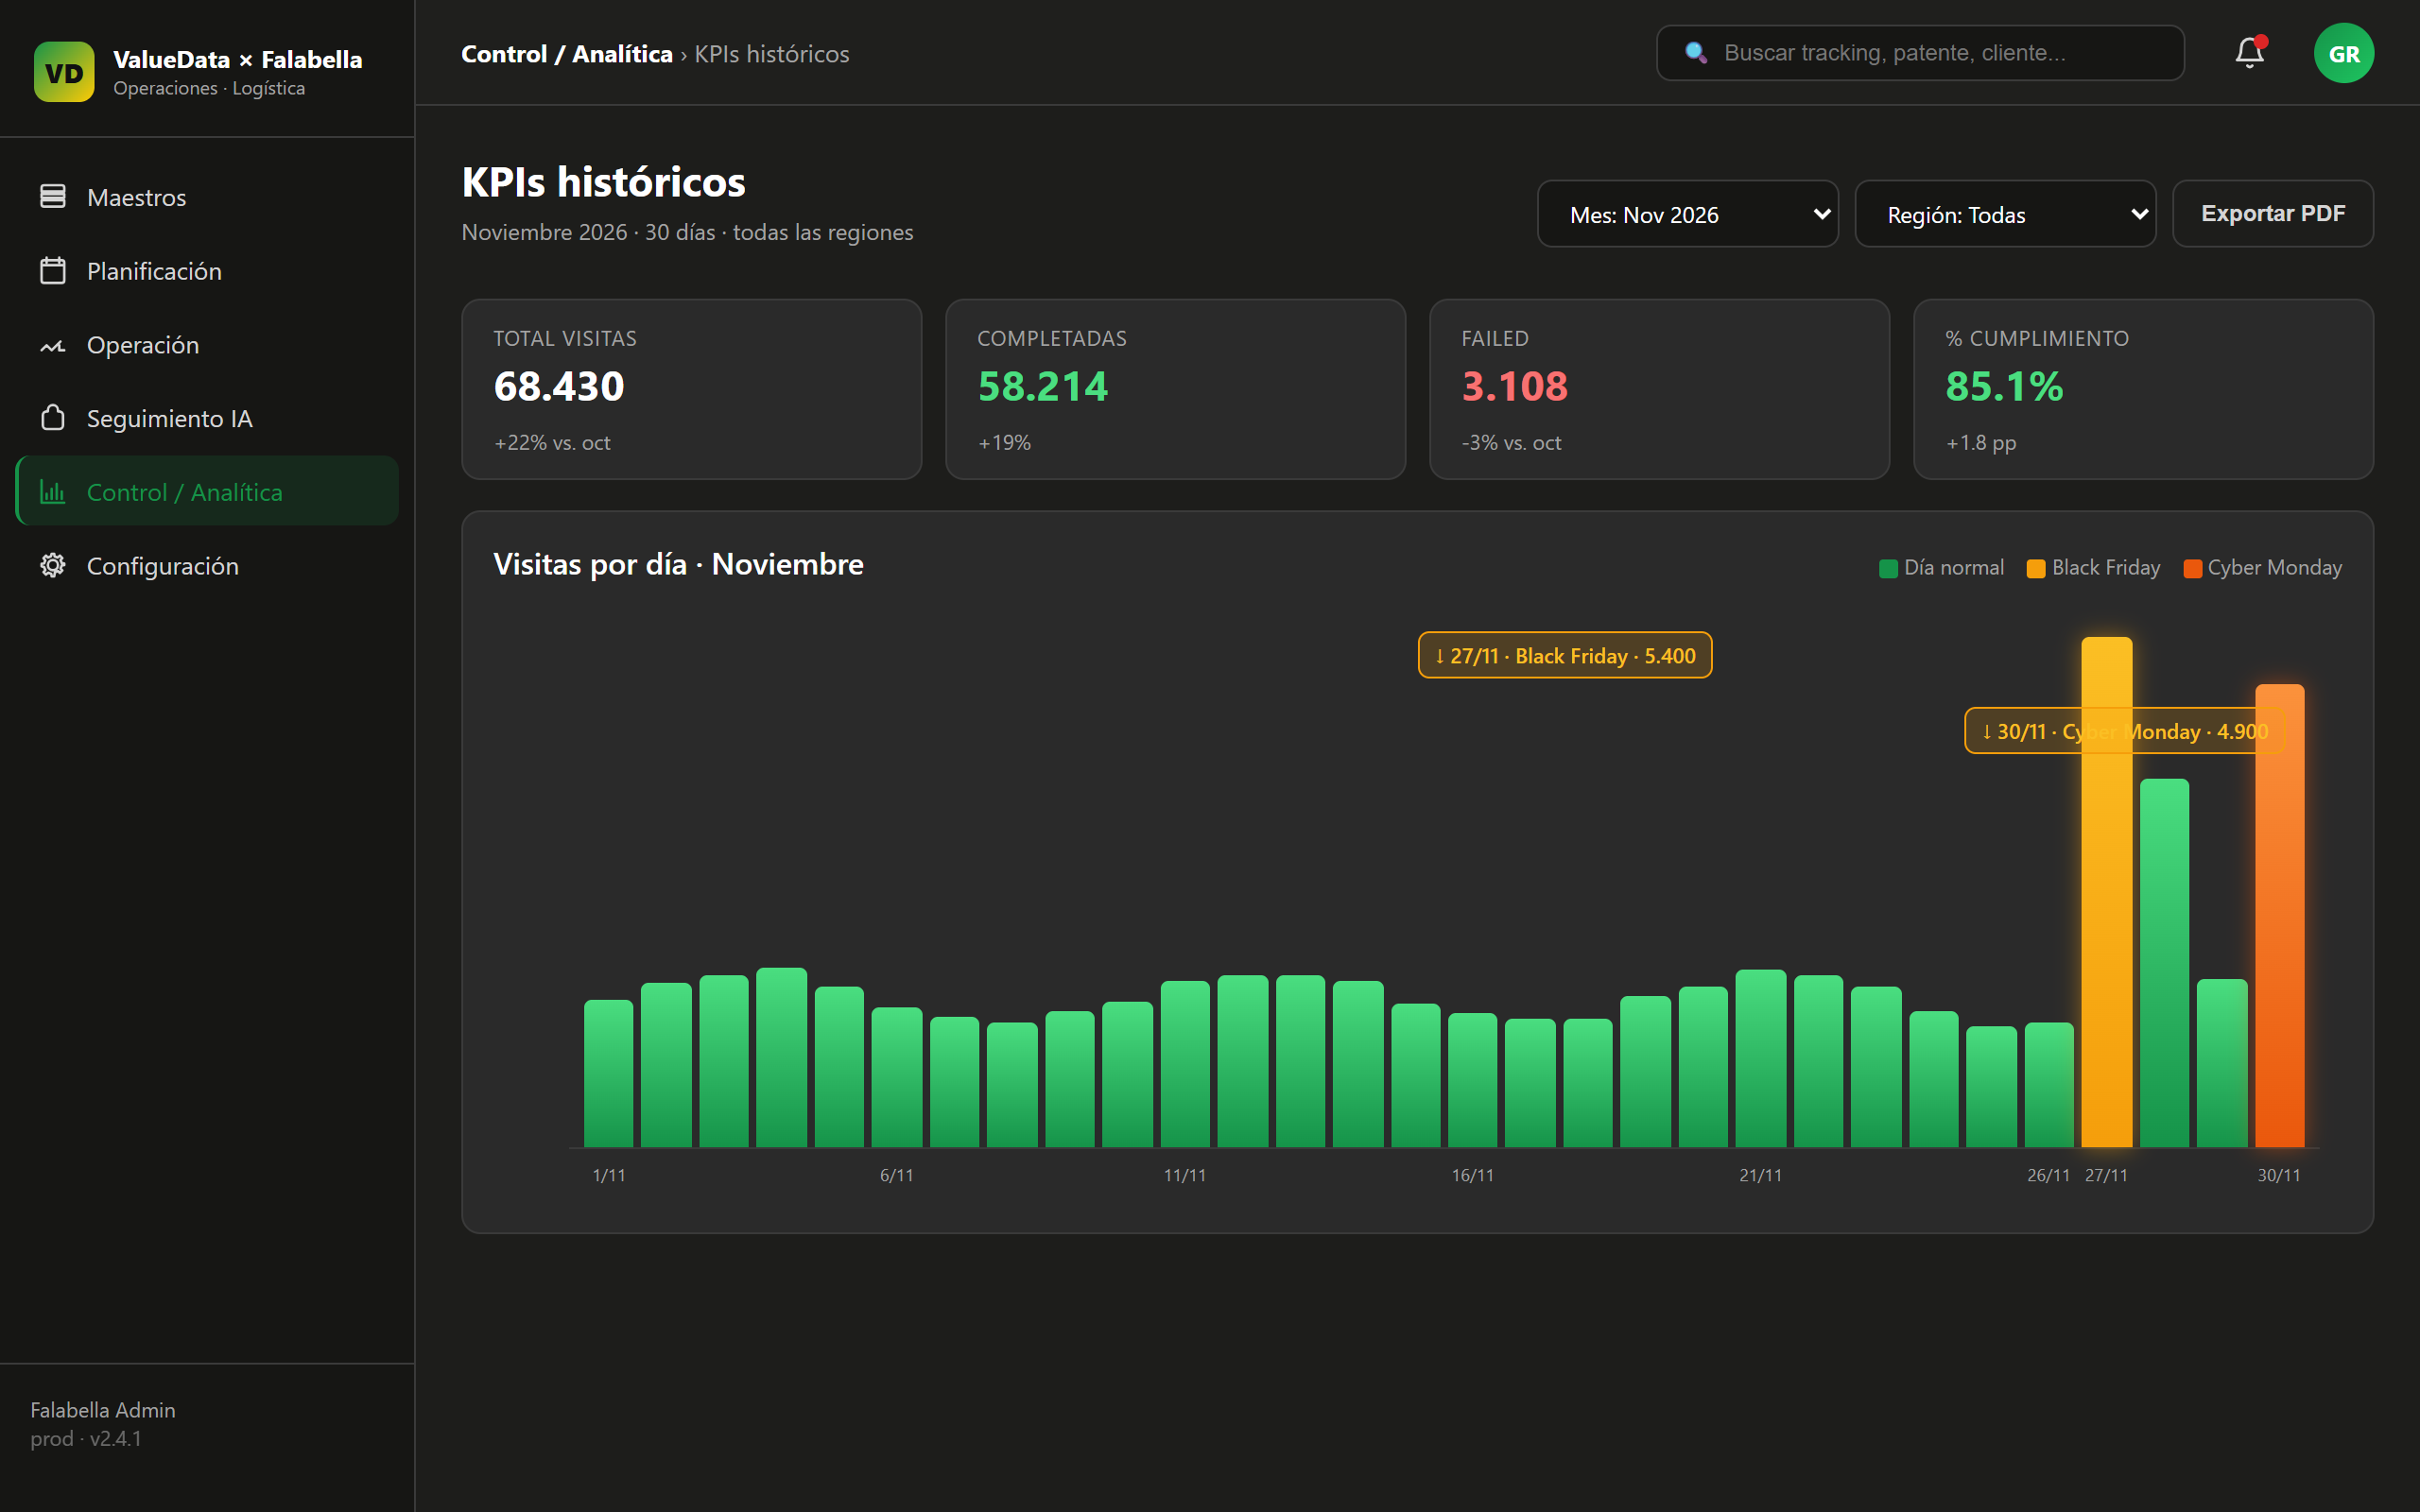
\includegraphics[width=0.95\textwidth]{13_kpis_historico.png}
\caption{KPIs historicos: 4 cards superiores (total / completadas / failed / \% cumplimiento) y grafico de barras de visitas por dia. En noviembre se ven los picos de Black Friday (27/11) y Cyber Monday (30/11) destacados en amarillo y naranja.}
\end{figure}

Pantalla con los KPIs del dia, semana, mes. Refresca cada 30 segundos.
Muestra:

\begin{itemize}
  \item Total de visitas, completadas, pendientes.
  \item Cantidad de alertas (rojas / amarillas SimpliRoute, alertas
        ValueData).
  \item Fallas reales del oraculo (cuando aplica), \% capturadas por
        ValueData.
  \item Suma esperada de fallos (\(\sum p_{fallo}\)).
  \item Compliance proyectado (\%): dado el modelo y el rate de
        rescate, cuantas visitas se van a completar.
  \item CLP rescatado: estimacion economica de las fallas evitadas
        gracias a las alertas anticipadas.
\end{itemize}

\subsection{Driver scorecard}

\begin{figure}[H]
\centering
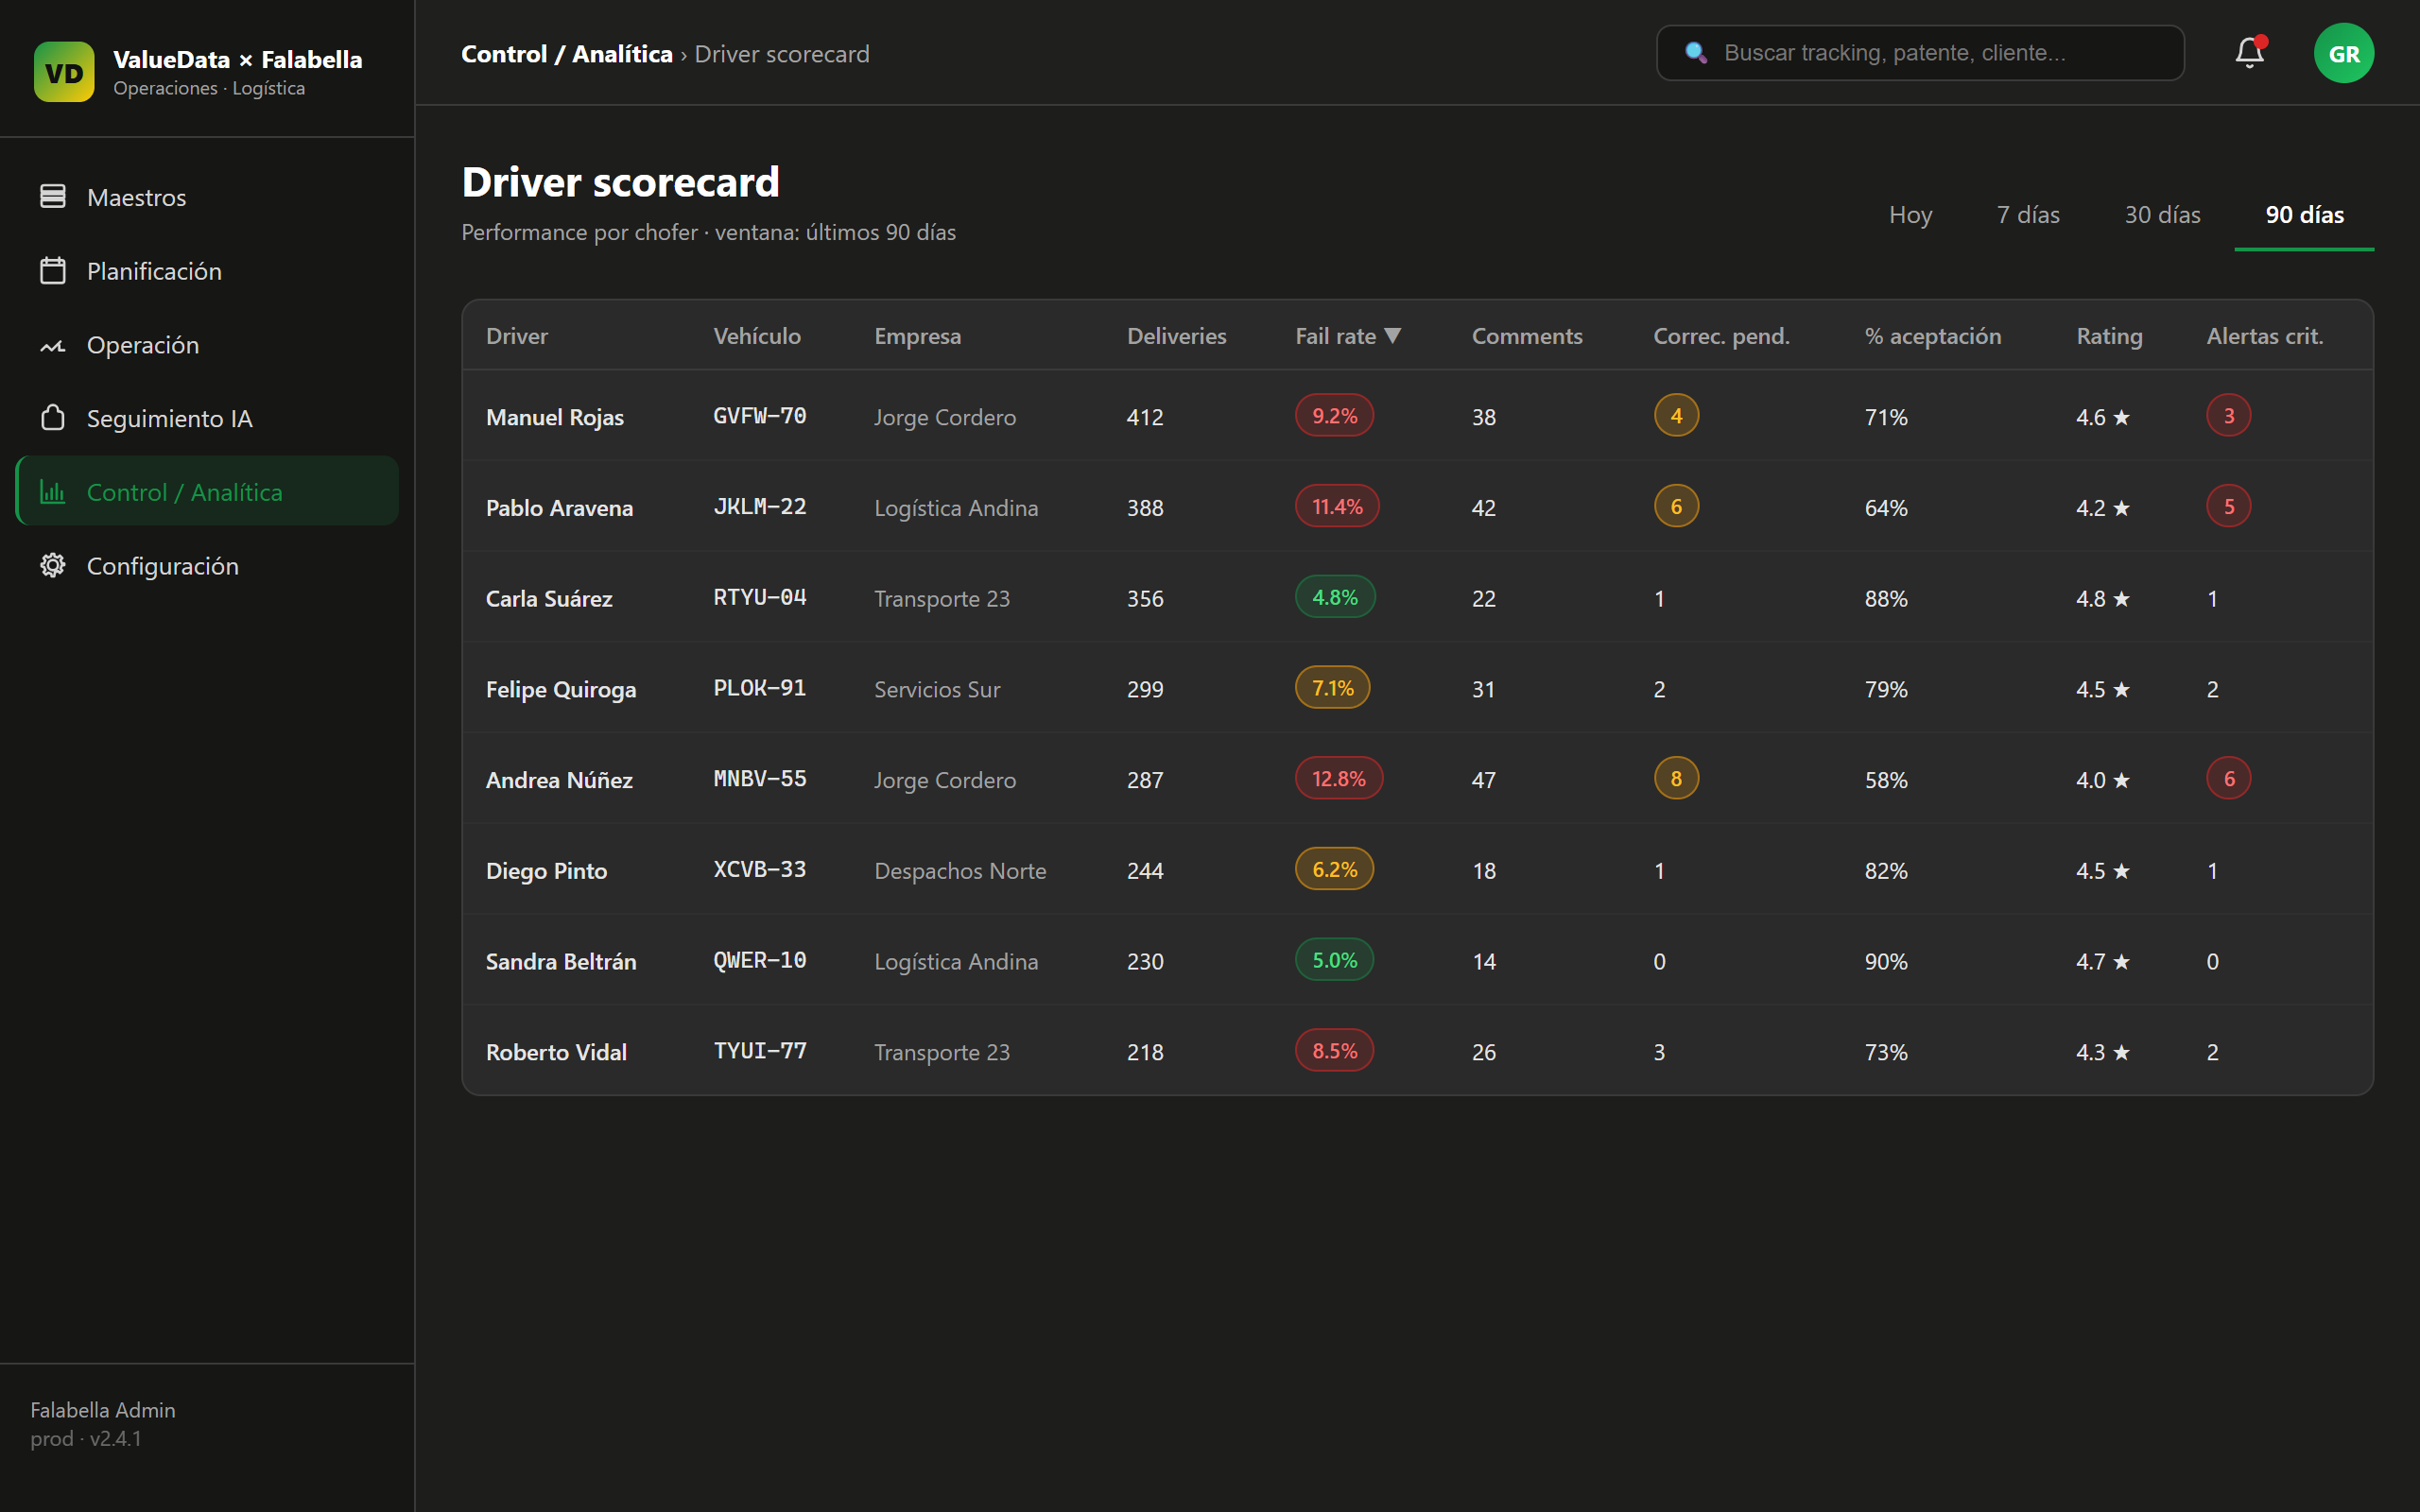
\includegraphics[width=0.95\textwidth]{12_driver_scorecard.png}
\caption{Driver scorecard: tabs de periodo (hoy / 7d / 30d / 90d) y tabla con deliveries, fail rate, comments, correcciones pendientes, \% aceptacion, rating y alertas criticas. Los fail rate $>$ 8\% se destacan en chip rojo.}
\end{figure}

Sidebar $\rightarrow$ Control / Analitica $\rightarrow$ Driver
scorecard. Tabla con un row por driver. Refresca cada 60 segundos.

\subsubsection{Periodos: Hoy / 7d / 30d / 90d}

Pills al tope de la pantalla. Click en uno cambia el periodo. La
metrica se recalcula sobre la ventana elegida.

\subsubsection{Metricas y ranking}

Columnas (todas ordenables por click en el header):

\begin{itemize}
  \item \textbf{Driver:} nombre, ID, foto.
  \item \textbf{Vehiculo:} nombre y patente.
  \item \textbf{Empresa:} a que transportista pertenece.
  \item \textbf{Entregas (n\_dias):} cantidad de visitas
        completadas en el periodo.
  \item \textbf{Fail rate:} \(\frac{fallidas}{entregas\_totales}\).
        Color rojo si $> 15\%$.
  \item \textbf{Comments:} cantidad total de motivos reportados.
  \item \textbf{Pendientes:} correcciones IA pendientes para sus
        comentarios.
  \item \textbf{\% acept.:} de las correcciones IA cerradas, cuantas
        terminaron \emph{accepted} (es decir, el chofer reporto mal y
        la IA tuvo razon). Mas alto = chofer reporta peor.
  \item \textbf{Rating:} estrellas del fleet (1--5).
  \item \textbf{Alertas criticas (n\_dias):} cuantas alertas critical
        genero el chofer en el periodo.
\end{itemize}

Click en una fila abre un drawer con detalle: lista de comentarios
recientes, correcciones pendientes, evolucion temporal del fail rate.

\subsection{Notificaciones log}

\begin{figure}[H]
\centering
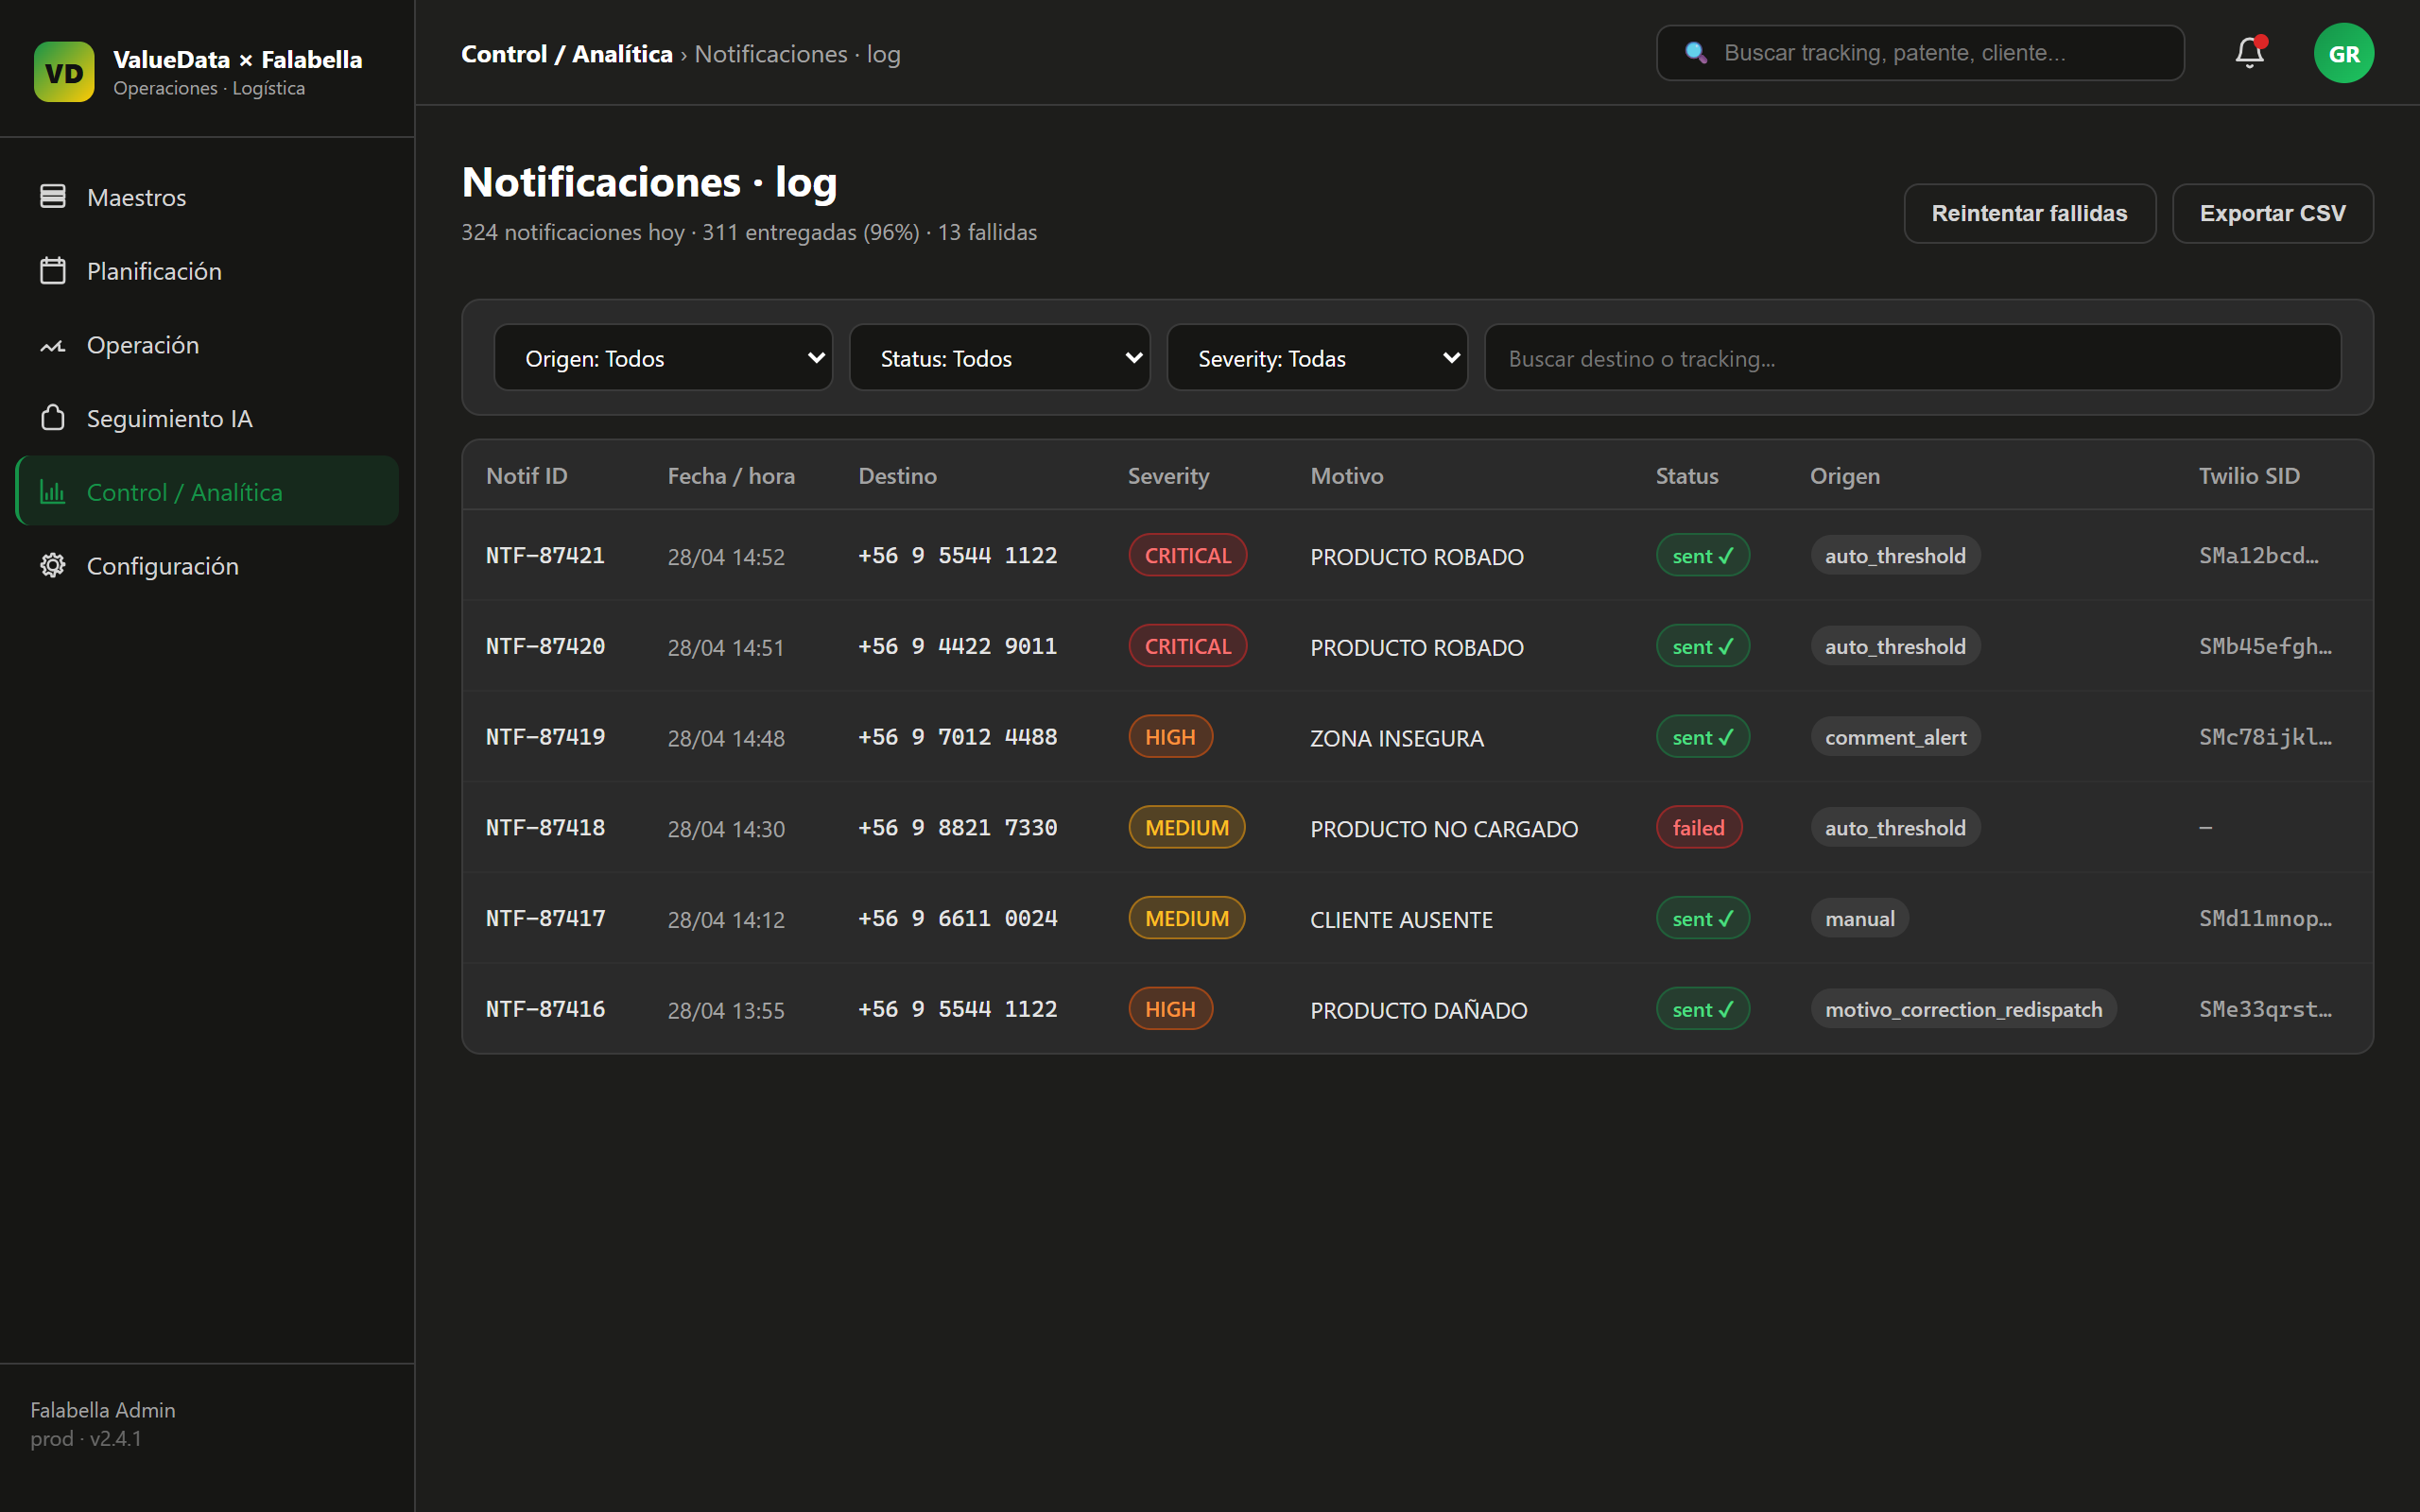
\includegraphics[width=0.95\textwidth]{14_notif_log.png}
\caption{Notificaciones log: filtros por origen (auto\_threshold, comment\_alert, manual, motivo\_correction\_redispatch) y por status. Cada fila muestra notification\_id, hora, destino, severity, motivo, status y el SID de Twilio para auditoria.}
\end{figure}

Tabla con todos los WhatsApp enviados por la plataforma. Columnas:
fecha/hora, tracking, motivo, severidad, destinatario (numero), tipo
(user / contacto / driver), estado Twilio (sent, delivered, read,
failed), trigger (\texttt{comment\_alert},
\texttt{vip\_deadline\_warning}, \texttt{motivo\_correction\_redispatch},
broadcast manual).

Filtros: rango de fecha, empresa, severidad, motivo, estado, trigger.
Util para auditoria y para diagnosticar por que alguien no recibio el
mensaje.

\subsection{Modelo XGBoost}

Pantalla tecnica para mostrar a Falabella la robustez del modelo.

\begin{itemize}
  \item \textbf{Metricas:} AUC, Brier score, matriz de confusion,
        curva de calibracion, base rate train/val.
  \item \textbf{Top features:} ranking de importancia (top 15 por
        defecto, ajustable). Cada feature tiene su nombre tecnico y un
        \emph{display} en lenguaje natural (ej.
        \texttt{slack\_min} $\rightarrow$ ``Holgura sobre la
        ventana'').
  \item \textbf{Calibration plot:} eje x probabilidad predicha en
        bins; eje y frecuencia observada. Idealmente sobre la
        diagonal.
\end{itemize}

% =============================================================================
\section{Modulo CONFIGURACION}
% =============================================================================

Sub-tabs: Alertas, WhatsApp / Twilio, LLM, Integraciones. En el POC
estos tabs son mayormente \textbf{informativos}: muestran el estado
actual del sistema y donde se configura cada cosa, pero no permiten
editar.

\subsection{Alertas globales}

\wipbox{Pantalla informativa. Por ahora la configuracion de alertas se
gestiona en \emph{Maestros $\rightarrow$ Catalogo motivos} (motivo a
motivo, alertable + severity por empresa). En el siguiente sprint se
agrega un panel global con: rate-limit por empresa, ventanas horarias
de no-disturbio, escalamiento por tiempo sin respuesta.}

\subsection{WhatsApp / Twilio}

Muestra el estado actual de la integracion:

\begin{itemize}
  \item \textbf{Provider:} Twilio.
  \item \textbf{Modo:} sandbox (numero \texttt{whatsapp:+14155238886}).
  \item \textbf{Para produccion:} cambiar
        \texttt{TWILIO\_WHATSAPP\_FROM} en el archivo \texttt{.env} del
        backend al numero verificado por Meta. Registrar templates
        oficiales para mensajes outbound.
\end{itemize}

\subsection{LLM (Azure OpenAI)}

Configuracion del clasificador:

\begin{itemize}
  \item \textbf{Modelo:} Azure OpenAI \texttt{gpt-4o-mini} (o el
        deployment configurado).
  \item \textbf{Variables de entorno requeridas:}
        \texttt{AZURE\_OPENAI\_ENDPOINT},
        \texttt{AZURE\_OPENAI\_API\_KEY},
        \texttt{AZURE\_OPENAI\_CHAT\_DEPLOYMENT}.
  \item \textbf{Fallback:} si la API esta caida, el sistema usa un
        clasificador por keywords basado en el catalogo. Permite no
        bloquear la operacion.
\end{itemize}

\subsection{Integraciones}

\wipbox{Conectores SimpliRoute (real, no mock), BigQuery, Slack y otros.
Disenados para el roadmap; no estan habilitados en el POC.}

% =============================================================================
\section{Flujos end-to-end (CASOS DE USO)}
% =============================================================================

Esta seccion describe paso a paso los escenarios reales que el cliente
Falabella va a vivir en operacion. Cada caso de uso lleva al usuario
desde el inicio hasta el cierre, con la pantalla y los clicks
exactos.

\subsection{Onboarding de empresa transportista}

\textbf{Objetivo:} dar de alta una empresa transportista nueva con
todo lo necesario para empezar a recibir alertas WhatsApp el mismo dia.

\textbf{Rol requerido:} Falabella admin.

\begin{enumerate}
  \item \textbf{Crear empresa.} Maestros $\rightarrow$ Empresas.
        Boton ``+ Nueva empresa''. Nombre comercial y empresa\_id (si
        no se asigna automaticamente). Activa = si.
  \item \textbf{Cargar contactos.} Maestros $\rightarrow$ Empresas y
        contactos. Click ``Ver contactos $\rightarrow$''. Pestana
        ``Importar CSV''. Descarga el template, lo llenas con los
        contactos del jefe de transporte, coordinadores, dispatchers
        principales. Sube el CSV.
  \item \textbf{Marcar opt-ins.} Para cada contacto cargado, haz clic
        en \emph{``marcar opt-in''}. (En produccion, cada contacto
        recibe el template de bienvenida y responde si.)
  \item \textbf{Test broadcast.} Pestana ``Test broadcast'' del
        drawer. Mensaje: \emph{``Test ValueData. Si recibes este
        mensaje, estas correctamente configurado.''}. Click Enviar.
        Verifica con el jefe de transporte que el mensaje llego.
  \item \textbf{Crear usuario manager.} Maestros $\rightarrow$
        Usuarios. ``+ Nuevo usuario''. Email del jefe de transporte,
        rol \texttt{transport\_manager}, empresa = la recien creada,
        password temporal. Marca \texttt{notify\_whatsapp} si quieres
        que tambien reciba alertas.
  \item \textbf{Comparte credenciales.} Envia al jefe la URL, su
        email, la password temporal y le pides que la cambie en su
        primer ingreso (cuando este flujo este disponible).
  \item \textbf{Configurar alertas por motivo (opcional).} Si la
        empresa tiene reglas distintas a la global, ve a Maestros
        $\rightarrow$ Catalogo motivos y crea overrides por empresa.
\end{enumerate}

\warnbox{Si saltas el paso 3 (opt-ins), los contactos quedan creados
pero NO reciben WhatsApp. Es un error frecuente.}

\subsection{Activar WhatsApp para un grupo de despacho}

\textbf{Objetivo:} configurar que un grupo de 5 despachadores de RM
reciba solo alertas critical y high de la empresa Transporte 02.

\textbf{Rol:} Falabella admin u Ops.

\begin{enumerate}
  \item Maestros $\rightarrow$ Empresas y contactos. Click en
        Transporte 02. ``Ver contactos''.
  \item Para cada despachador, ``+ Agregar contacto'' (o cargalos por
        CSV).
  \item En el formulario:
    \begin{itemize}
      \item Rol: \texttt{dispatcher}.
      \item Phone: numero E.164.
      \item Severidades: marca \texttt{critical} y \texttt{high}.
      \item Region: \texttt{RM}.
    \end{itemize}
  \item Guarda. Repite para los 5.
  \item ``marcar opt-in'' para los 5.
  \item Test broadcast con un mensaje breve. Verifica que los 5
        recibieron.
  \item Listo. A partir de ahora, una visita en RM con motivo critical
        o high de Transporte 02 dispara WhatsApp a los 5
        automaticamente.
\end{enumerate}

\subsection{Marcar cliente como VIP con hora limite}

\textbf{Objetivo:} cliente ``Empresas Sodimac S.A.'' debe recibir
antes de las 16:00, con alerta 90 minutos antes si esta en riesgo.

\textbf{Rol:} Falabella admin.

\begin{enumerate}
  \item Maestros $\rightarrow$ Clientes VIP. ``+ Nuevo VIP''.
  \item Tipo de match: \texttt{title}. Tier: \texttt{VIP-PLATA}.
  \item Valor: copia exacta de la razon social como aparece en las
        visitas (\emph{Empresas Sodimac S.A.}). El match es exacto.
  \item Empresa: \emph{Global} (vacio) si aplica a todas las
        transportistas; o elige una si solo le entrega una.
  \item Notas: \emph{``Cliente VIP, entregar antes de las 4 PM con
        90 minutos de aviso.''}.
  \item Click en \textbf{``Sugerir desde notas''}. La IA rellena
        deadline\_time = 16:00 y alert\_minutes\_before = 90.
  \item Verifica los valores. Marca Activo = si.
  \item Crear VIP.
  \item A partir de aqui, cada dia el cron VIP revisa si alguna visita
        de Sodimac corre riesgo de pasarse de las 16:00 y dispara la
        alerta a las 14:30.
\end{enumerate}

\subsection{Chofer reporta motivo de no-entrega}

\begin{figure}[H]
\centering
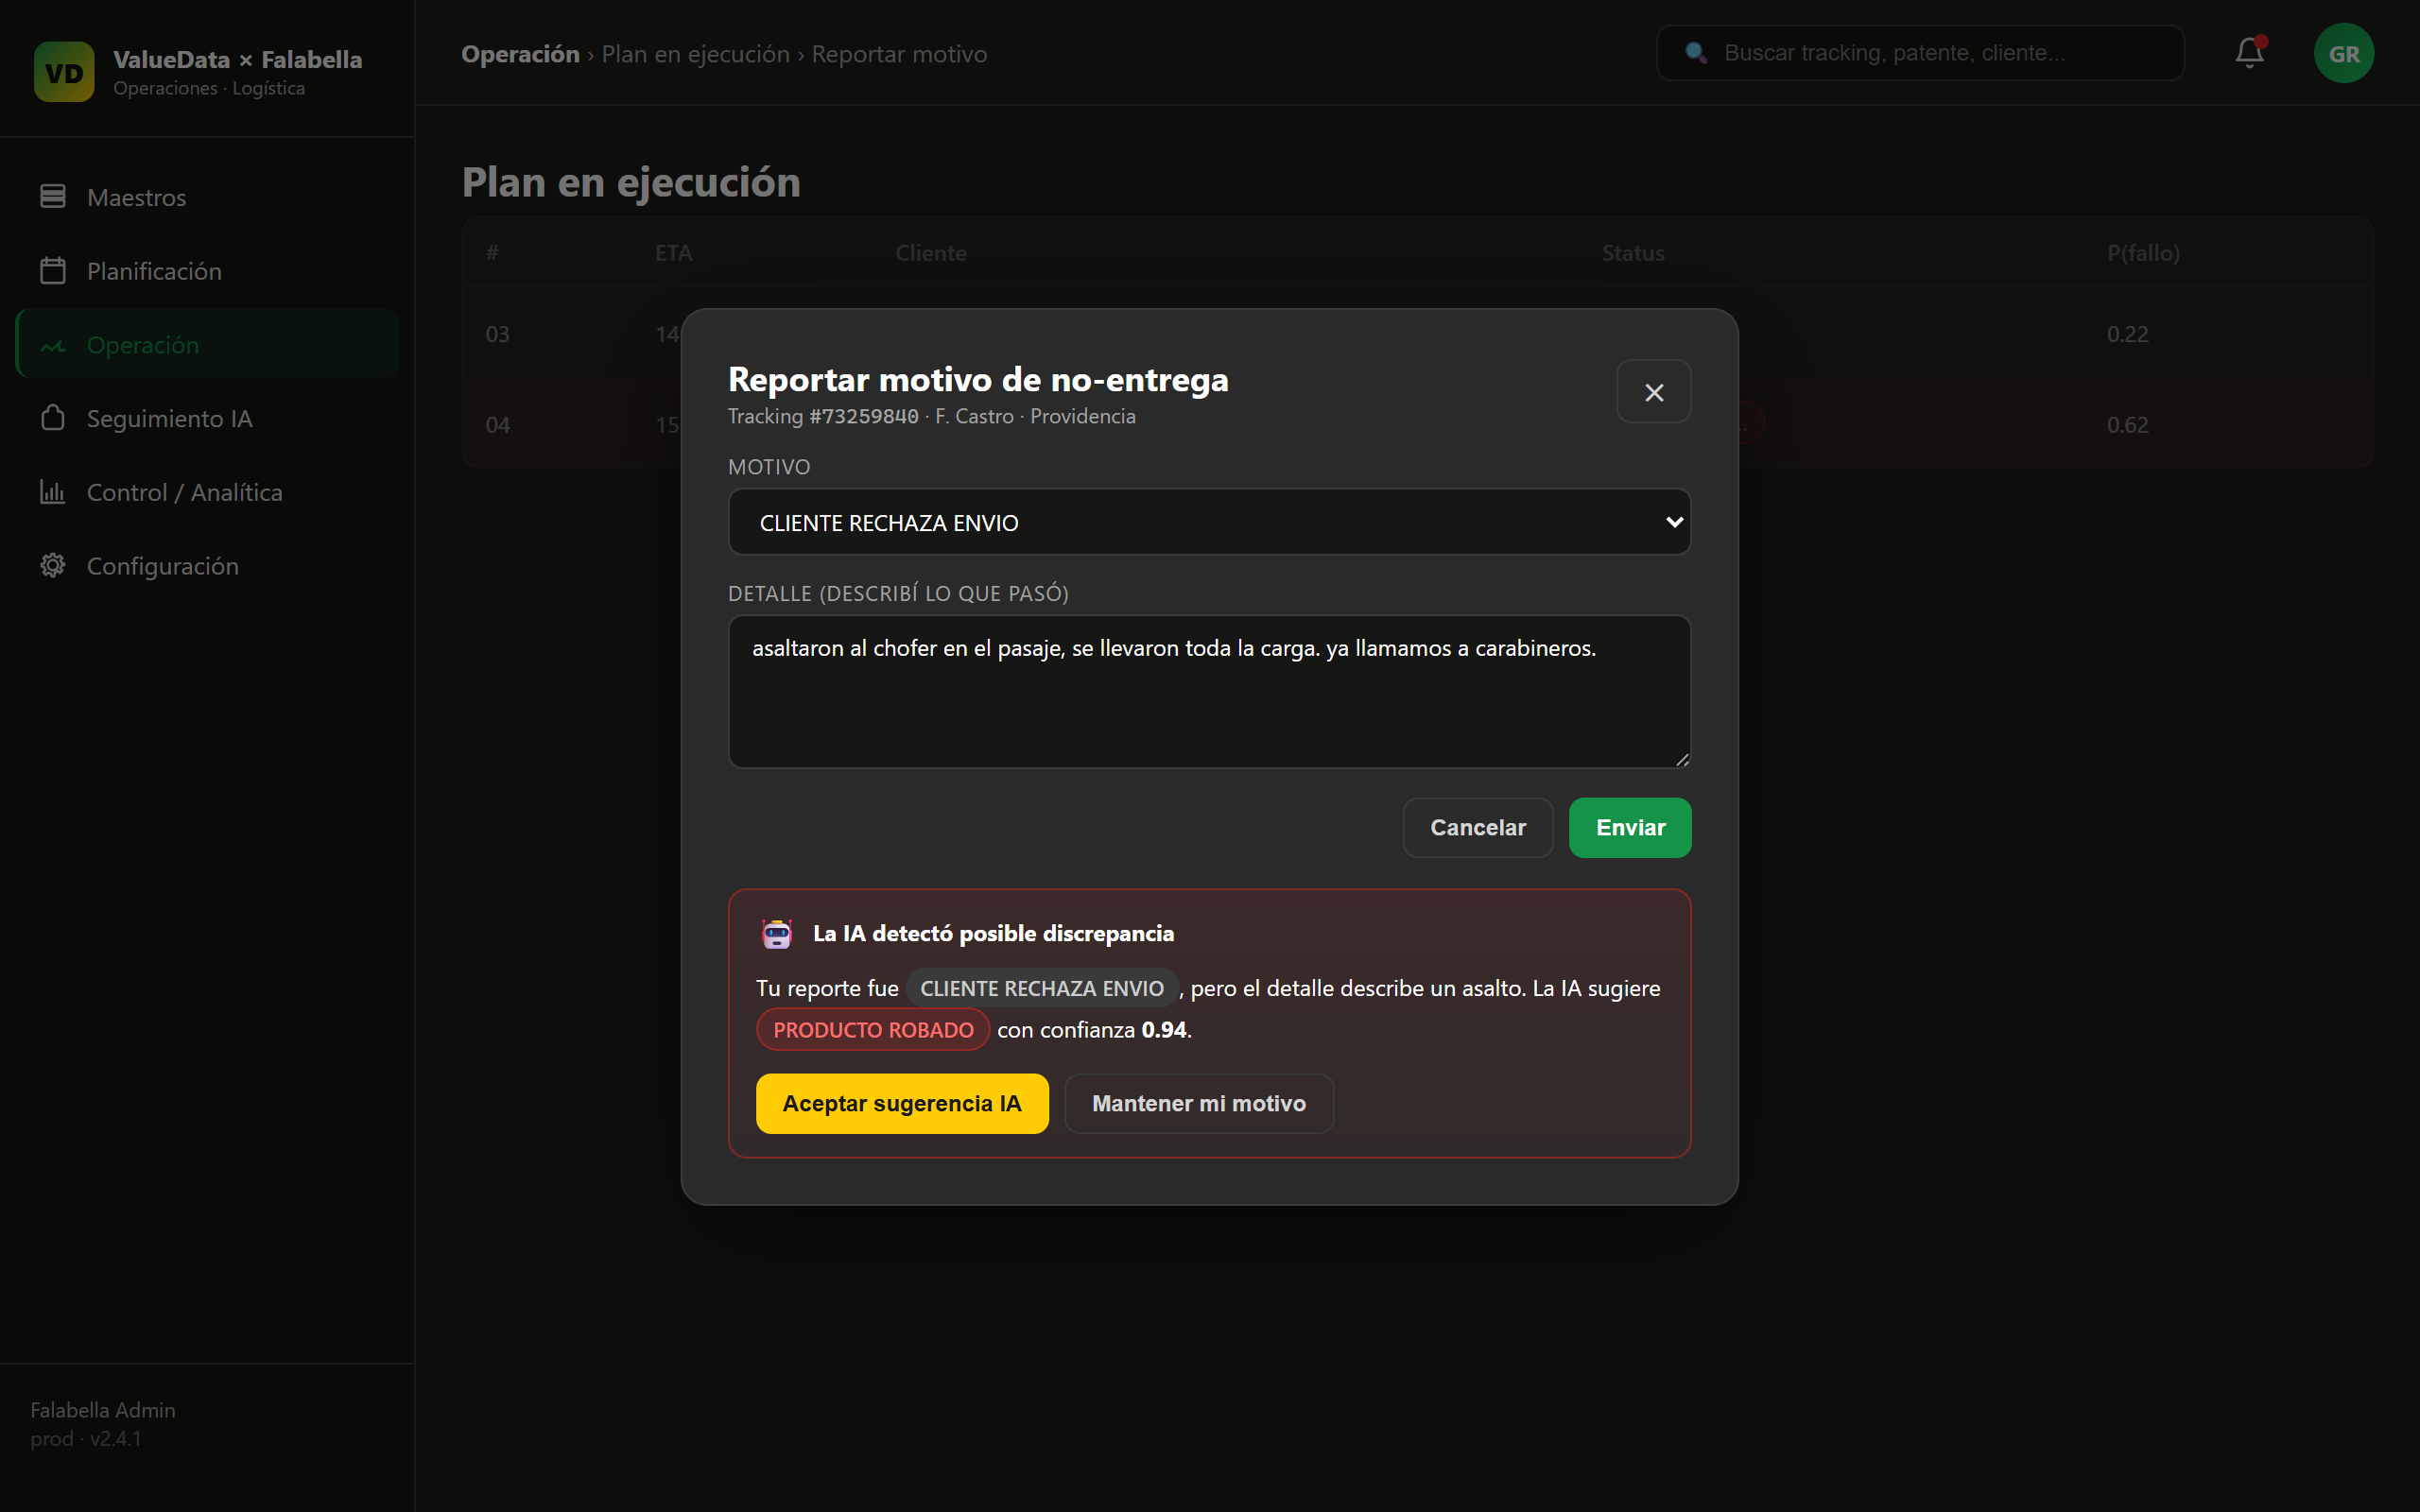
\includegraphics[width=0.9\textwidth]{15_reportar_motivo.png}
\caption{Modal Reportar motivo: dropdown con los 13 motivos del catalogo, textarea de detalle y botones Cancelar / Enviar. Al detectar discrepancia (texto describe robo pero el motivo elegido es CLIENTE RECHAZA ENVIO), aparece el aviso de la IA proponiendo PRODUCTO ROBADO con confianza 0.94.}
\end{figure}

\textbf{Objetivo:} el chofer Juan llega a una direccion mal
geolocalizada y no puede entregar.

\textbf{Rol:} Manager transportista (o Ops Falabella en su nombre).

\begin{enumerate}
  \item Operacion $\rightarrow$ Plan en ejecucion. Localiza la visita
        (filtra por driver Juan, o usa el buscador global).
  \item Click en el icono de \textbf{megafono} (Reportar motivo).
  \item En el dialogo, motivo: \texttt{PROBLEMA DE DIRECCION/ SIN
        INFORMACION}.
  \item Comentario: \emph{``Direccion no existe. El cliente vive en
        un pasaje sin numeracion. Le llame y reagendamos manana.''}.
  \item Click Guardar.
  \item El backend persiste, dispara WhatsApp a quien corresponda
        (si el motivo esta marcado alertable: si, severity medium por
        defecto), y llama al LLM para validar.
  \item En la fila de la visita aparece la insignia del motivo y se
        actualiza el contador de fallidas en la barra de KPIs.
\end{enumerate}

\subsection{La IA detecta motivo mal categorizado --- admin acepta correccion}

\textbf{Objetivo:} un chofer reporto \texttt{SIN MORADORES} pero el
comentario dice ``Camion choco contra una moto, hay carabineros, no
puedo seguir''. La IA detecta que es \texttt{SINIESTRO EN CALLE}.

\textbf{Rol:} Falabella admin/ops.

\begin{enumerate}
  \item Recibes una notificacion en la campana de la topbar:
        \emph{``Revision IA''}. Tambien aparece en
        Operacion $\rightarrow$ Alertas en vivo y en
        Seguimiento IA $\rightarrow$ Comentarios recientes.
  \item Ve a Seguimiento IA $\rightarrow$ Correcciones de motivo.
        Pestana \emph{Pendientes}.
  \item Localiza la fila. Columnas:
    \begin{itemize}
      \item Tracking: \texttt{FAL-2026-04-28-XXXXXX}.
      \item Reportado: \texttt{SIN MORADORES}.
      \item IA sugiere: \texttt{SINIESTRO EN CALLE} (chip rojo).
      \item Confianza: \emph{alta} (chip verde).
      \item Razonamiento: \emph{``El comentario menciona accidente y
            carabineros. Esto corresponde a SINIESTRO EN CALLE, no a
            ausencia de moradores''}.
      \item Comentario original (en italica).
    \end{itemize}
  \item Click en \textbf{Aceptar} (check verde).
  \item El backend:
    \begin{enumerate}
      \item Aplica \texttt{SINIESTRO EN CALLE} al comentario original.
      \item Marca la correccion como \emph{accepted}.
      \item Calcula severidades: \texttt{SIN MORADORES} no es
            alertable. \texttt{SINIESTRO EN CALLE} es critical.
            $\Rightarrow$ \emph{escalado}.
      \item Re-dispatch: envia WhatsApp critical a admins, ops, manager
            de la empresa, contactos opt-in que matcheen.
    \end{enumerate}
  \item En la UI, la correccion pasa a la pestana \emph{Aceptadas}.
        En Operacion $\rightarrow$ Alertas en vivo aparece un evento
        \texttt{motivo\_correction\_decided} con
        \texttt{redispatched=true}.
  \item Carabineros, despachador y supervisor reciben el WhatsApp
        critical en sus telefonos.
\end{enumerate}

\subsection{Black Friday --- como se ven los picos en KPIs}

\textbf{Objetivo:} entender como se comporta la torre de control en
un dia de pico (Black Friday, Cyber, Navidad).

\textbf{Rol:} Cualquier rol Falabella.

\begin{enumerate}
  \item En la mañana, Sidebar $\rightarrow$ Control / Analitica
        $\rightarrow$ KPIs. Tipicamente vas a ver:
    \begin{itemize}
      \item Total de visitas 2x--3x el dia normal.
      \item Cantidad de alertas anticipadas (\texttt{vd\_alerts})
            crece proporcionalmente.
      \item Compliance proyectado baja a 78--82\% (vs 90\%+ normal)
            por la presion en el sistema.
    \end{itemize}
  \item Operacion $\rightarrow$ Watchlist. Vas a ver mucho rojo. Usa
        el filtro \emph{VIP en riesgo} para priorizar.
  \item Operacion $\rightarrow$ Mapa. Detecta zonas con concentracion
        de puntos rojos: ahi hay que reforzar con vehiculos extras o
        coordinar con el transportista.
  \item Seguimiento IA $\rightarrow$ Comentarios recientes. Si la
        cantidad de comentarios alertables es atipicamente alta (mas
        de 30 por hora), revisa que motivos predominan. Tipicamente
        en pico aparecen mas \texttt{PROD N ENTREGADO X TIEMPO} y
        \texttt{FUERA DE COBERTURA/ FRECUENCIA}.
  \item Control / Analitica $\rightarrow$ Notificaciones log. Verifica
        que los WhatsApp se estan enviando. Si ves muchos
        \emph{failed}, llama a soporte porque puede haber rate limit
        de Twilio.
  \item Control / Analitica $\rightarrow$ Driver scorecard, periodo
        \emph{Hoy}. Identifica los drivers con fail rate $> 25\%$ y
        derivalos al manager para refuerzo.
\end{enumerate}

\tipbox{El dia siguiente al pico, comparar con el periodo \emph{30
dias} permite ver si los problemas son estructurales (siempre fallan
ahi) o coyunturales (fueron solo de ese dia). Eso ayuda a tomar
decisiones de capacidad.}

% =============================================================================
\section{Sistema de alertas WhatsApp}
% =============================================================================

\begin{figure}[H]
\centering
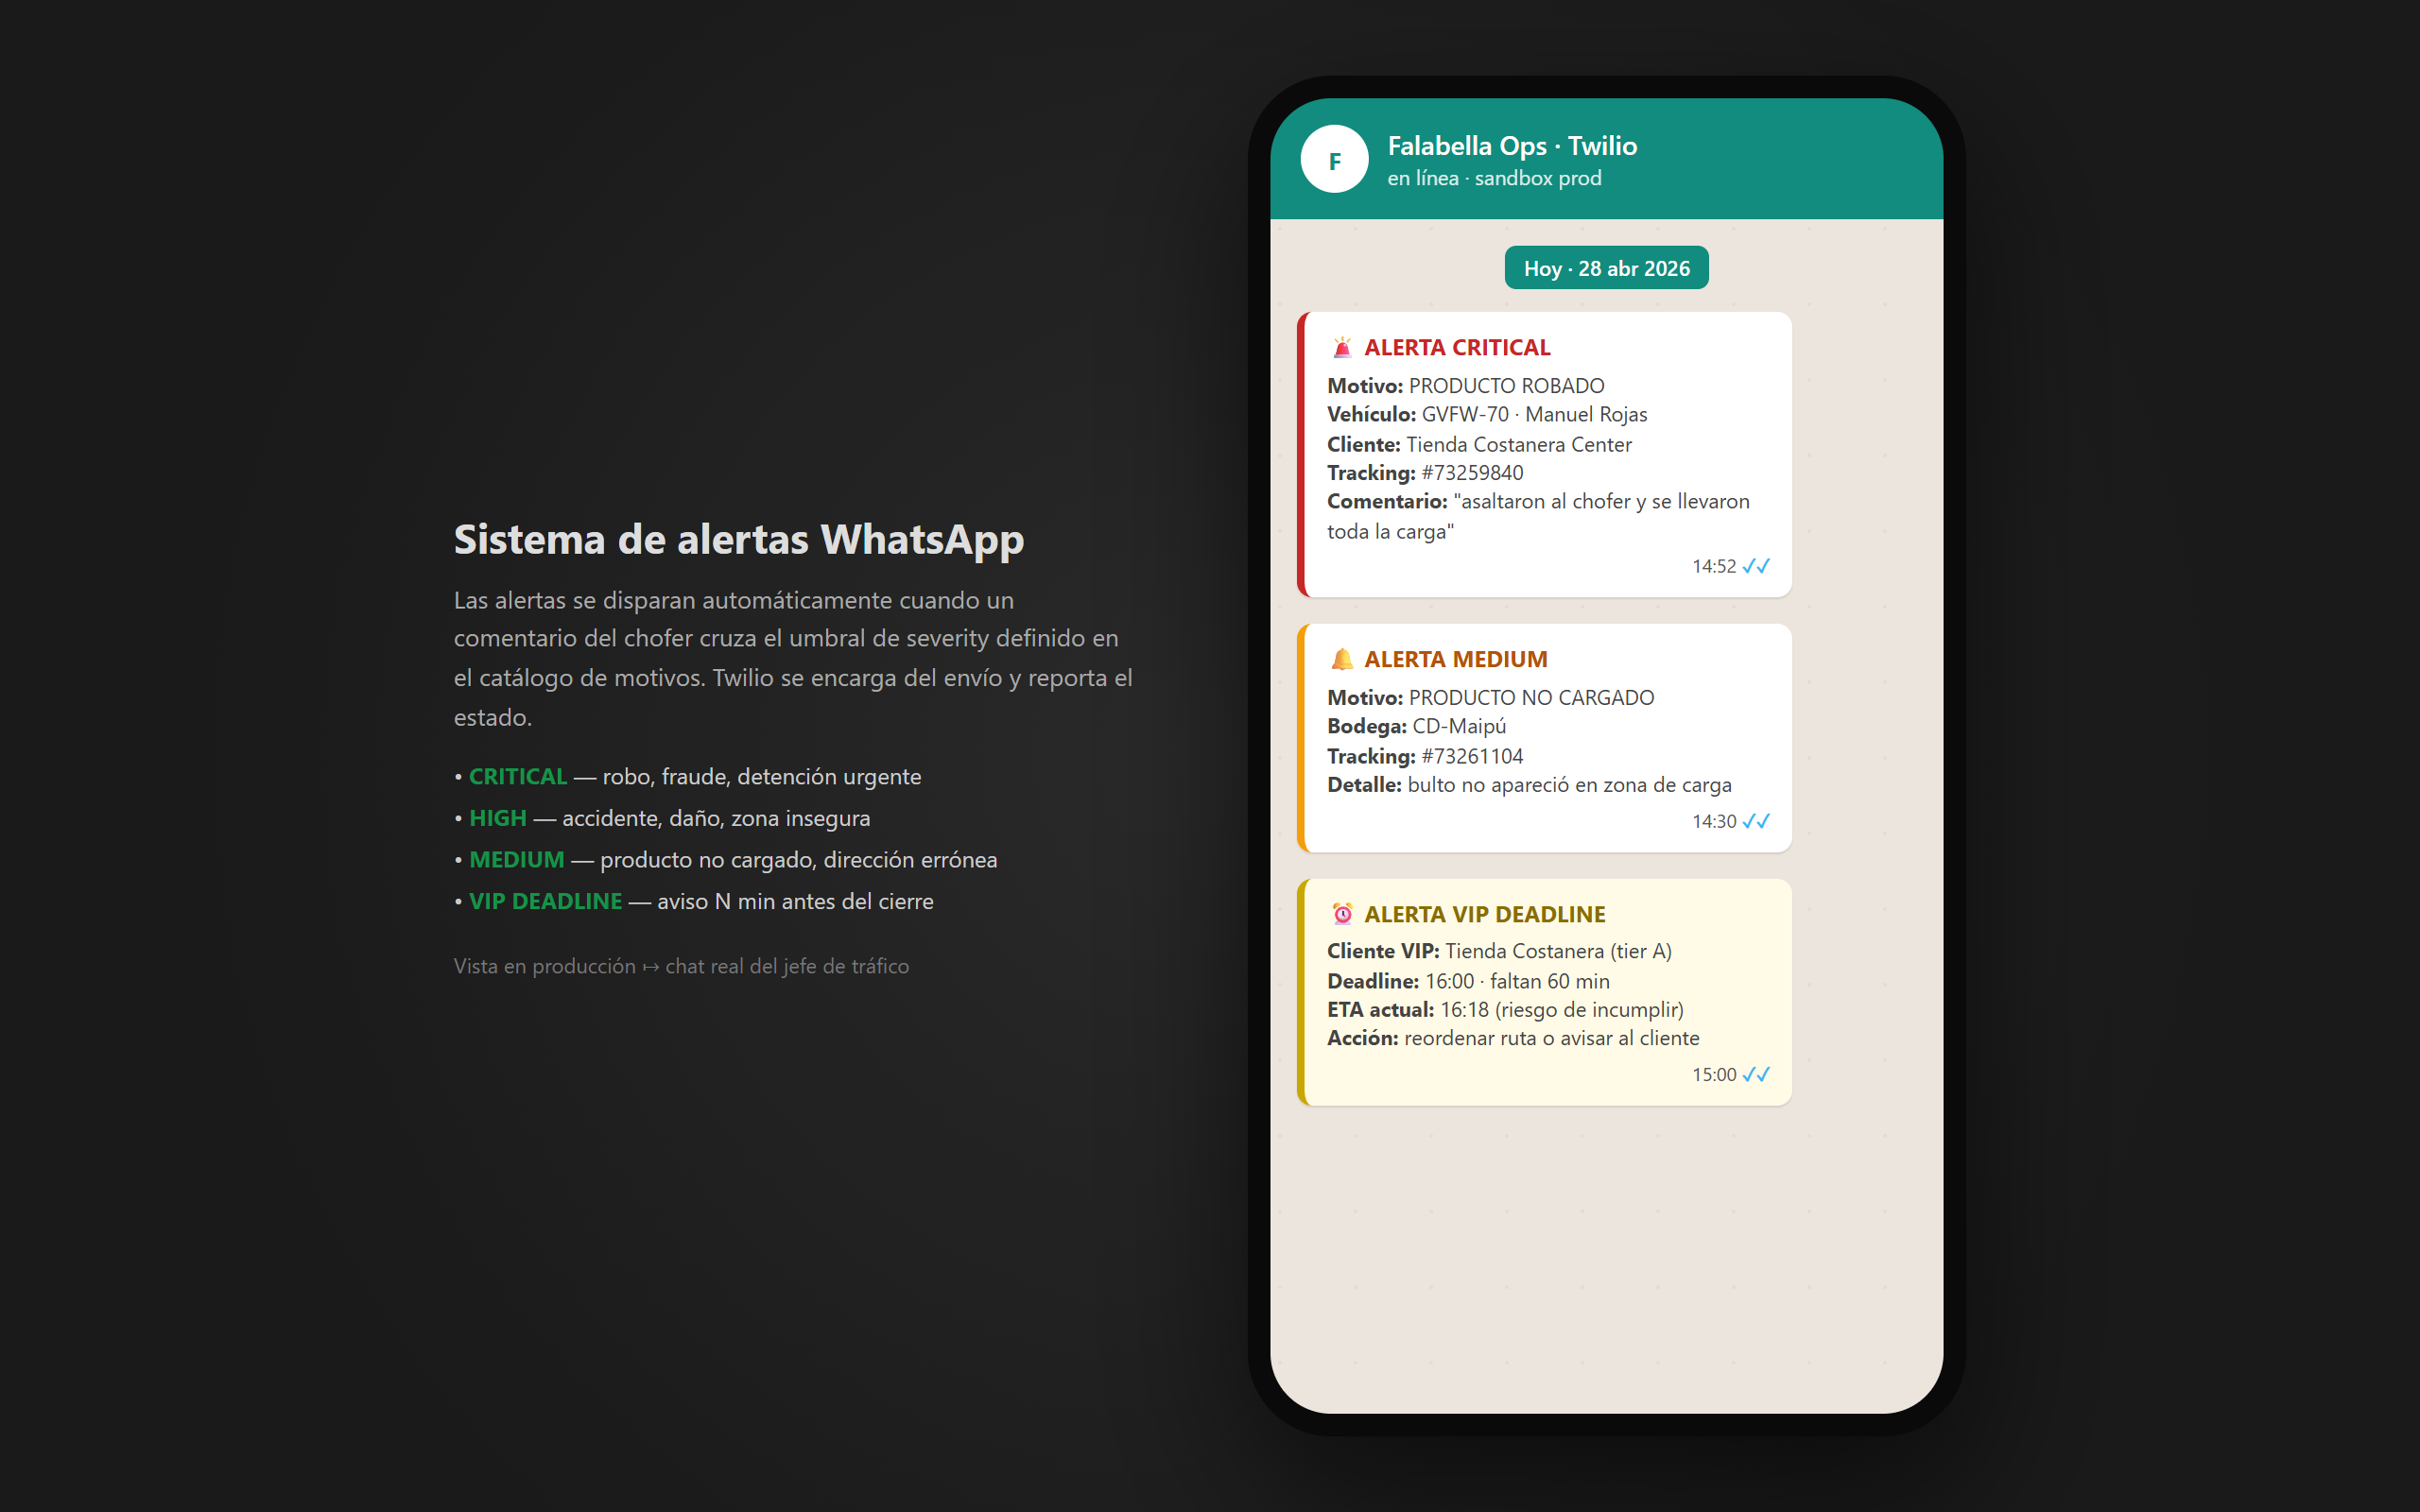
\includegraphics[width=0.95\textwidth]{16_whatsapp_chat.png}
\caption{Vista de las alertas tal como llegan al WhatsApp del jefe de trafico: encabezado verde Falabella Ops via Twilio, tres burbujas tipicas (CRITICAL por siniestro, MEDIUM por producto no cargado y VIP DEADLINE) con timestamp y check de entrega.}
\end{figure}

\subsection{Cuando se dispara una alerta}

Hay tres triggers principales:

\begin{enumerate}
  \item \textbf{\texttt{comment\_alert}:} cuando un chofer reporta un
        motivo configurado como \emph{alertable} para esa empresa
        (override) o globalmente.
  \item \textbf{\texttt{vip\_deadline\_warning}:} cuando una visita VIP
        entra en la ventana \emph{deadline $-$ alert\_minutes\_before}
        sin haberse completado.
  \item \textbf{\texttt{motivo\_correction\_redispatch}:} cuando un
        admin acepta una correccion IA y la severidad efectiva escala.
\end{enumerate}

A esto se suma el \textbf{broadcast manual} desde el panel Test
Broadcast (ver Seccion 5.1).

\subsection{Quien la recibe (logica del fan-out)}

El backend resuelve la lista de destinatarios en funcion de tres
fuentes, con prioridad:

\begin{enumerate}
  \item \textbf{Users login:} \texttt{fpoc\_users} con
        \texttt{notify\_whatsapp=1}, \texttt{activo=1} y phone valido.
        Filtra a \texttt{falabella\_admin/ops} (siempre) o a managers
        de la empresa de la visita.
  \item \textbf{Contactos de la empresa:} \texttt{fpoc\_empresa\_contactos}
        con \texttt{active=1} y \texttt{opted\_in\_at} no nulo,
        filtrados por la empresa de la visita.
  \item \textbf{Drivers de la empresa:} \texttt{fpoc\_drivers} con
        \texttt{active=1}, \texttt{notify\_whatsapp=1},
        \texttt{opted\_in\_at} no nulo, asignados a un vehiculo de la
        empresa.
\end{enumerate}

\textbf{Deduplicacion:} si un mismo numero aparece en mas de una
fuente, se cuenta una sola vez. La fuente \emph{users} tiene
prioridad (porque tiene \texttt{user\_id} para auditoria).

\subsection{Filtros por severity, motivo, region}

Cada contacto tiene tres listas configurables:

\begin{itemize}
  \item \texttt{severities\_in}: si esta vacio, recibe todas. Si tiene
        valores (ej. \texttt{["high","critical"]}), recibe solo esos.
  \item \texttt{motivos\_in}: si esta vacio, recibe todos. Si tiene
        valores, recibe solo esos.
  \item \texttt{region\_filter}: \texttt{RM}, \texttt{regiones} o
        \texttt{all}. La region de la visita se determina por
        \texttt{region} si viene en el dataset, o por bounding box
        lat/lon de RM como fallback.
\end{itemize}

\subsection{Estado del sandbox vs produccion}

\textbf{POC (sandbox):}
\begin{itemize}
  \item Twilio sandbox \texttt{whatsapp:+14155238886}.
  \item Receptores deben previamente enviar \emph{``join
        \textit{<sandbox-code>}''} al numero sandbox para autorizarse.
  \item Limite: \(\sim\)50 mensajes por dia, sin templates.
\end{itemize}

\textbf{Produccion:}
\begin{itemize}
  \item Numero verificado por Meta (BSP).
  \item Templates aprobados para outbound.
  \item Sin limite practico (segun plan Twilio).
  \item Costo por mensaje. La torre de control solo dispara cuando es
        relevante (con filtros), por lo que el costo se controla.
\end{itemize}

\warnbox{En sandbox, si un destinatario no se unio al numero, el
mensaje no llega y aparece como \emph{failed} en el log. Esto es
esperado y no es bug.}

% =============================================================================
\section{Modelo XGBoost (lectura no tecnica)}
% =============================================================================

\subsection{Que hace}

El modelo XGBoost predice, para cada visita planificada del dia, la
probabilidad de que esa visita \textbf{no se complete} dentro de la
ventana de tiempo prometida. Devuelve un numero entre 0 y 1: por
ejemplo, \(p_{fallo}=0.78\) significa que el modelo cree que hay un
78\% de chance de que esa visita falle.

El modelo se entrena cada vez que arranca el backend (toma 30--40
segundos) usando datos historicos. En produccion se reentrenara con
periodicidad acordada con Falabella (semanal o mensual).

\subsection{Como lee la nota de riesgo}

Las features que mas influyen en \(p_{fallo}\) (top 5 tipico):

\begin{enumerate}
  \item \textbf{Holgura sobre la ventana} (\texttt{slack\_min}): cuanto
        margen tiene la visita antes de cerrar la ventana. Negativo =
        ya se paso.
  \item \textbf{Atraso observado del vehiculo}
        (\texttt{\_obs\_delay}): cuantos minutos viene retrasado el
        vehiculo respecto del plan SimpliRoute.
  \item \textbf{Carga del vehiculo}: vehiculos sobrecargados tienden a
        atrasarse mas.
  \item \textbf{Hora del dia}: el final del turno tiene mas riesgo.
  \item \textbf{Zona / cliente}: cliente con historia de no-entregas
        tiene mas riesgo.
\end{enumerate}

\subsection{Por que confiar en el (calibracion + SHAP)}

\begin{itemize}
  \item \textbf{Calibracion:} el modelo no solo ranquea, sino que sus
        probabilidades estan calibradas. Si dice 80\%, en la practica
        80 de 100 casos similares fallan. La curva de calibracion en
        Control / Analitica $\rightarrow$ Modelo XGB lo demuestra.
  \item \textbf{SHAP por visita:} para cada alerta, el sistema explica
        que features contribuyeron mas. Esto se ve en el detalle de
        cada alerta anticipada (\texttt{top\_factors}). Asi un
        operador no recibe una alerta opaca sino una alerta
        \emph{razonada}.
  \item \textbf{AUC y Brier:} las metricas tipicas estan en la pantalla
        del modelo y se monitorean en cada reentrenamiento. Si bajan,
        es senal de que el modelo se degrado y hay que revisar los
        datos.
\end{itemize}

% =============================================================================
\section{Preguntas frecuentes}
% =============================================================================

\subsection{Por que no llega el WhatsApp?}

Causas comunes, en orden:

\begin{enumerate}
  \item \textbf{Sin opt-in.} El contacto esta creado pero no tiene
        \texttt{opted\_in\_at}. Solucion: en Maestros $\rightarrow$
        Empresas y contactos, marca opt-in (POC) o pide al destinatario
        que responda \emph{si} al template (produccion).
  \item \textbf{Sandbox no autorizado.} En POC, los destinatarios deben
        haber enviado \emph{``join \textit{<sandbox-code>}''} al numero
        sandbox de Twilio. Si no, los mensajes aparecen como
        \emph{failed}.
  \item \textbf{Filtros no matchean.} El contacto tiene severidades o
        motivos restringidos y la alerta no corresponde a esa lista.
        Solucion: revisa los filtros del contacto.
  \item \textbf{Region no matchea.} Contacto con \texttt{region=RM} y
        la visita es en regiones (o viceversa).
  \item \textbf{Phone mal formateado.} No es E.164. El log de Twilio
        marca \emph{invalid number}. Solucion: edita el contacto.
  \item \textbf{Twilio rate limit.} En picos, Twilio puede aplicar rate
        limit. Revisa Notificaciones log; si ves muchos \emph{failed
        429}, contactar soporte Twilio.
\end{enumerate}

\tipbox{Para diagnosticar, ve a Control / Analitica $\rightarrow$
Notificaciones log y filtra por el tracking o el numero. La columna
\emph{estado} te dice exactamente que paso.}

\subsection{Como agrego una nueva empresa transportista?}

Ver Seccion 11.1 \emph{Onboarding de empresa transportista}. Resumen:
crear empresa, cargar contactos por CSV, marcar opt-ins, test
broadcast, crear usuario manager, configurar overrides de motivos si
aplica.

\subsection{Que hago si el LLM clasifica mal?}

\begin{enumerate}
  \item \textbf{Caso aislado:} en
        Seguimiento IA $\rightarrow$ Correcciones, \textbf{rechaza} la
        sugerencia. El motivo original se mantiene.
  \item \textbf{Patron recurrente:} si el LLM siempre confunde dos
        motivos, mejora la \textbf{descripcion operacional} de ambos
        en Maestros $\rightarrow$ Catalogo motivos. Agrega ejemplos
        \emph{``NO usar si: \dots $\rightarrow$ MOTIVO\_X''}.
  \item Cierra sesion y reingresa para verificar el cambio (el LLM
        usa la descripcion en cada llamada nueva).
\end{enumerate}

\subsection{Como cambio la hora deadline de un VIP?}

\begin{enumerate}
  \item Maestros $\rightarrow$ Clientes VIP. Localiza el VIP por su
        razon social (usa el buscador global).
  \item Click en \textbf{Editar} (lapiz azul).
  \item Cambia el campo \emph{Hora limite (HH:MM)}.
  \item Opcionalmente, ajusta \emph{Alertar minutos antes} si quieres
        cambiar la antelacion.
  \item Guardar cambios.
  \item El cron VIP toma el nuevo valor en la siguiente corrida (60s).
\end{enumerate}

\subsection{Puedo editar el catalogo de motivos?}

\textbf{Los 13 motivos no se pueden agregar ni borrar.} Vienen del
notebook de auditoria operacional de Falabella y son la base del
clasificador.

\textbf{Lo que si se puede editar} es, para cada motivo:
\begin{itemize}
  \item Si es alertable o no (global o por empresa).
  \item Su severidad (low/medium/high/critical, global o por empresa).
  \item Su descripcion operacional (lo que el LLM ve para clasificar).
\end{itemize}

% =============================================================================
\section{Glosario}
% =============================================================================

\begin{longtable}{p{3.6cm} p{12.0cm}}
\toprule
\textbf{Termino} & \textbf{Definicion} \\
\midrule
\endhead
\texttt{tracking\_id} & Identificador unico de una visita (entrega).
  Formato \texttt{FAL-YYYY-MM-DD-XXXXXX}. \\
\texttt{ruta\_id} & Identificador de la ruta del dia
  (vehiculo + fecha). Aparece en el header de cada ruta del plan en
  ejecucion. \\
ETA & \emph{Estimated Time of Arrival.} Hora estimada de llegada a la
  visita. \\
\texttt{slack\_min} & Holgura en minutos entre la ETA y el cierre de
  la ventana de entrega. Negativo = atraso confirmado. \\
\texttt{p\_fallo} & Probabilidad (0--1) de que la visita falle, segun
  el modelo XGBoost. \\
\texttt{alert\_slack} & Semaforo de holgura: GREEN, YELLOW, RED. \\
\texttt{alert\_valuedata} & True si la combinacion de
  $p_{fallo}$ y la ventana califica como alerta anticipada. \\
severity & Nivel de severidad de un motivo: low, medium, high, critical. \\
fan-out & Logica que multiplica un evento (alerta) hacia muchos
  destinatarios filtrados. \\
opt-in & Aceptacion explicita del receptor para recibir mensajes
  WhatsApp. Requerido por Twilio y Meta. \\
sandbox Twilio & Ambiente de pruebas de Twilio para WhatsApp; gratis
  pero limitado, requiere \emph{``join $<$code$>$''} en cada destinatario. \\
BSP & \emph{Business Solution Provider} de Meta para WhatsApp. Twilio
  es uno. \\
template Meta & Plantilla pre-aprobada por Meta para enviar mensajes
  outbound (fuera de la ventana de 24h del usuario). \\
SHAP & \emph{SHapley Additive exPlanations.} Tecnica para explicar la
  contribucion de cada feature a una prediccion individual. \\
AUC & \emph{Area Under the Curve} (ROC). Mide la capacidad del modelo
  para separar fallos de no-fallos. 1.0 perfecto, 0.5 azar. \\
Brier score & Metrica de calidad de probabilidades. Mas bajo, mejor. \\
deadline\_time & Hora limite de un VIP (HH:MM). \\
alert\_minutes\_before & Minutos antes del deadline VIP en que se
  dispara la alerta de riesgo. \\
empresa transportista & Tercero que opera vehiculos para entregar las
  visitas de Falabella. Cada vehiculo pertenece a una empresa. \\
breadcrumb & Texto en la topbar que indica donde estas (Modulo /
  Sub-tab). \\
sub-tab & Pestana secundaria dentro de un modulo. \\
\bottomrule
\end{longtable}

% =============================================================================
\section{Apendices}
% =============================================================================

\subsection*{Apendice A. Comandos curl utiles para admin}
\addcontentsline{toc}{subsection}{Apendice A. Comandos curl utiles para admin}

Para diagnostico rapido o automatizacion. Reemplaza
\texttt{TOKEN} por el JWT obtenido del login.

\textbf{A.1. Login (obtener JWT):}

\begin{lstlisting}
curl -X POST http://localhost:8090/api/auth/login \
  -H "Content-Type: application/json" \
  -d '{"email":"admin@falabella.cl","password":"admin123"}'
\end{lstlisting}

\textbf{A.2. Listar alertas anticipadas:}

\begin{lstlisting}
curl http://localhost:8090/api/alerts/anticipated?limit=20 \
  -H "Authorization: Bearer TOKEN"
\end{lstlisting}

\textbf{A.3. KPIs del dia:}

\begin{lstlisting}
curl http://localhost:8090/api/kpis \
  -H "Authorization: Bearer TOKEN"
\end{lstlisting}

\textbf{A.4. Catalogo de motivos con config alertable / severity:}

\begin{lstlisting}
curl http://localhost:8090/api/motivos/alert-config \
  -H "Authorization: Bearer TOKEN"
\end{lstlisting}

\textbf{A.5. Crear comentario en una visita (test de motivo):}

\begin{lstlisting}
curl -X POST http://localhost:8090/api/visits/FAL-2026-04-28-XXXXXX/comment \
  -H "Authorization: Bearer TOKEN" \
  -H "Content-Type: application/json" \
  -d '{"motivo":"SINIESTRO EN CALLE","comentario":"Choque en ruta 5"}'
\end{lstlisting}

\textbf{A.6. Ver correcciones pendientes:}

\begin{lstlisting}
curl http://localhost:8090/api/motivo-corrections?status=pending&limit=50 \
  -H "Authorization: Bearer TOKEN"
\end{lstlisting}

\textbf{A.7. Aceptar una correccion IA:}

\begin{lstlisting}
curl -X POST http://localhost:8090/api/motivo-corrections/123/accept \
  -H "Authorization: Bearer TOKEN"
\end{lstlisting}

\subsection*{Apendice B. Estados posibles de una visita}
\addcontentsline{toc}{subsection}{Apendice B. Estados posibles de una visita}

\begin{longtable}{p{3.0cm} p{12.5cm}}
\toprule
\textbf{Estado} & \textbf{Significado} \\
\midrule
\endhead
\texttt{pending} & Aun no fue completada. Es la mayoria al inicio del
  dia. \\
\texttt{completed} & Entregada exitosamente. \\
\texttt{failed} & Marcada como no-entregada (con o sin motivo
  reportado). \\
\texttt{in\_route} & En ruta hacia el cliente (no se usa en este POC,
  reservado para integracion real con SimpliRoute). \\
\texttt{cancelled} & Anulada antes del despacho. \\
\bottomrule
\end{longtable}

\subsection*{Apendice C. Severity levels}
\addcontentsline{toc}{subsection}{Apendice C. Severity levels}

\begin{longtable}{p{2.5cm} p{4.0cm} p{8.5cm}}
\toprule
\textbf{Nivel} & \textbf{Color UI} & \textbf{Cuando se usa} \\
\midrule
\endhead
low & Slate / gris &
  Eventos informativos, sin impacto operativo inmediato. \\
medium & Ambar / amarillo &
  Eventos que requieren atencion pero no son urgentes (ej. PROBLEMA
  DE DIRECCION). \\
high & Naranja &
  Requieren accion en el dia (ej. PRODUCTO NO CARGADO, DETENCION
  URGENTE). \\
critical & Rojo &
  Requieren accion inmediata (ej. SINIESTRO EN CALLE, PRODUCTO ROBADO,
  RIESGO FRAUDE). \\
\bottomrule
\end{longtable}

El \emph{rank} numerico es: low=0, medium=1, high=2, critical=3. Se
usa para detectar escalado en el flujo de correcciones IA.

\subsection*{Apendice D. Lista de los 13 motivos del catalogo con descripciones}
\addcontentsline{toc}{subsection}{Apendice D. Lista de los 13 motivos del catalogo con descripciones}

Estas son las descripciones operacionales por defecto que ve el LLM.
Pueden personalizarse por empresa en Maestros $\rightarrow$ Catalogo
motivos.

\textbf{D.1. SIN MORADORES} (default: \emph{no alertable}).
Nadie disponible en domicilio. Cliente no atiende, no responde
llamado/timbre. NO usar si el problema es la direccion (\texttt{PROBLEMA
DE DIRECCION}). NO usar si el cliente atendio pero rechazo
(\texttt{CLIENTE RECHAZA ENVIO}).

\textbf{D.2. PROBLEMA DE DIRECCION/ SIN INFORMACION} (default:
\emph{alertable, medium}).
Direccion erronea, mal escrita, inexistente, sin numeracion, no
ubicable, mal geolocalizada, sin informacion de contacto. NO usar si
la zona no es atendida (\texttt{NO DESPACHA} o \texttt{FUERA DE
COBERTURA}). NO usar si la direccion estaba bien pero no habia nadie
(\texttt{SIN MORADORES}).

\textbf{D.3. NO DESPACHA A LOCALIDAD} (default: \emph{no alertable}).
La direccion del cliente esta fuera de la zona geografica que la
empresa atiende. Aun cuando el cliente anula al darse cuenta, la causa
raiz sigue siendo no-despacho.

\textbf{D.4. FUERA DE COBERTURA/ FRECUENCIA} (default: \emph{no
alertable}). La ruta no llega a esa zona en el dia/horario actual.
Frecuencia insuficiente, fuera de ruta del dia.

\textbf{D.5. PROD N ENTREGADO X TIEMPO} (default: \emph{no alertable}).
No se alcanzo a entregar dentro del tiempo. Atraso, fin de turno.
\emph{CONDUCTOR NO GESTIONA} cae aca cuando es por gestion de tiempo.
NO usar si hubo siniestro (\texttt{SINIESTRO EN CALLE}). NO usar si el
producto nunca subio al camion (\texttt{PRODUCTO NO CARGADO}).

\textbf{D.6. PRODUCTO NO CARGADO} (default: \emph{alertable, high}).
El producto no fue cargado al vehiculo en origen. Quedo en bodega, no
se cargo por capacidad, fue olvidado.

\textbf{D.7. CLIENTE RECHAZA ENVIO} (default: \emph{no alertable}).
El cliente esta disponible y rechaza recibir: anula, no quiere,
devuelve, cancela. ATENCION: si el cliente anula porque la direccion
estaba mal, la causa raiz NO es rechazo --- es \texttt{PROBLEMA DE
DIRECCION} o \texttt{NO DESPACHA}.

\textbf{D.8. SINIESTRO EN CALLE} (default: \emph{alertable, critical}).
Eventos en ruta: asalto, robo, encerrona, accidente, choque, panne,
intervencion de carabineros.

\textbf{D.9. PRODUCTO CON PROBLEMAS} (default: \emph{no alertable}).
Producto roto, danado, embalaje en mal estado, faltante, incompleto.

\textbf{D.10. NO CUMPLE CONDICIONES RETIRO} (default: \emph{no
alertable}). El destinatario no cumple los requisitos: falta
documentacion (RUT, autorizacion), no acredita identidad.

\textbf{D.11. PRODUCTO ROBADO} (default: \emph{alertable, critical}).
El producto fue robado/sustraido de la carga.

\textbf{D.12. RIESGO FRAUDE} (default: \emph{alertable, critical}).
Pedido sospechoso de fraude (datos del cliente, RUT clonado, direccion
de phishing, intento de estafa, comportamiento inusual). NO entregar.
Reportar inmediatamente. NO usar si el cliente solo rechaza por
arrepentimiento (\texttt{CLIENTE RECHAZA ENVIO}). NO usar si hay
siniestro fisico (\texttt{SINIESTRO EN CALLE}).

\textbf{D.13. DETENCION URGENTE} (default: \emph{alertable, high}).
Detencion inmediata de la entrega ordenada por Falabella o transporte
(alerta judicial, cancelacion administrativa post-pickup, retencion por
aduana, etc.). NO entregar y devolver al CD. NO usar si el cliente
rechaza personalmente (\texttt{CLIENTE RECHAZA ENVIO}).

\subsection*{Apendice E. Glosario de roles}
\addcontentsline{toc}{subsection}{Apendice E. Glosario de roles}

\begin{longtable}{p{4.5cm} p{11.0cm}}
\toprule
\textbf{Rol} & \textbf{Descripcion} \\
\midrule
\endhead
\texttt{falabella\_admin}
  & Administrador global. Gestiona todo: empresas, motivos, VIPs,
    usuarios, dia simulado. \\
\texttt{falabella\_ops}
  & Operaciones de torre. Misma visibilidad que admin pero sin permisos
    para crear usuarios o resetear el dia. \\
\texttt{transport\_manager}
  & Jefe de operaciones de una empresa transportista. Ve solo lo
    relacionado con su \texttt{empresa\_id}. \\
contacto (no-user)
  & Persona registrada en \texttt{fpoc\_empresa\_contactos} para
    recibir alertas WhatsApp. No tiene acceso a la app. Roles:
    jefe, coordinador, dispatcher, driver, otro. \\
driver (chofer)
  & Conductor de un vehiculo. Tiene registro en \texttt{fpoc\_drivers};
    puede tener opcionalmente phone con opt-in para recibir alertas
    de su empresa o pedidos de validacion IA. \\
\bottomrule
\end{longtable}

\vspace{1cm}

\begin{center}
\rule{0.6\linewidth}{0.4pt}\\[0.3cm]
{\small Fin del manual --- ValueData $\times$ Falabella, abril 2026.}
\end{center}

\end{document}
